\documentclass{article}
% Shared preamble for main.tex and supp.tex (X-regularization, arXiv split).
% \input by both documents after their own \documentclass.
\usepackage[letterpaper, margin=1in]{geometry}
\usepackage{setspace}
\usepackage{amsmath,amssymb}
\usepackage{graphicx}
\usepackage{subcaption}
\usepackage[amsmath,thmmarks,framed]{ntheorem}
\usepackage{authblk}
\usepackage{tcolorbox}
\usepackage{booktabs}
\usepackage{multirow}
\usepackage{placeins}
\usepackage{enumerate}
\usepackage{xcolor}
\definecolor{darkgreen}{rgb}{0.0,0.5,0.0}
\usepackage[colorlinks,linkcolor=red,citecolor=darkgreen,urlcolor=blue]{hyperref}
\usepackage{xr-hyper}   % cross-document references between main.tex and supp.tex (must follow hyperref)
\usepackage[round,authoryear]{natbib}

\usepackage[ruled,linesnumbered]{algorithm2e}
\SetKwInput{KwInput}{Input}
\SetKwInput{KwOutput}{Output}

\newtheorem*{remark}{Remark}
\newtheorem{lemma}{Lemma}
\newtheorem{theorem}{Theorem}
\newenvironment{proof}{\par\medskip\noindent\textit{Proof.}\ }{\hfill$\square$\par\medskip}

\newcommand{\Le}{\leqslant}
\newcommand{\Ge}{\geqslant}
\newcommand{\D}{\mathrm{d}}
\newcommand{\KL}{\mathrm{KL}}
\newcommand{\X}{\mathrm{X}}
\newcommand{\ESS}{\mathrm{ESS}}

\theoremstyle{plain}


\title{Forward KL Can Be Better: Normalizing Flow Boltzmann Sampling with Log-Ratio Variation}
\author[1]{Qi Feng}
\author[2]{Rongjie Lai}
\author[2]{Di Qi}
\author[2]{Xuda Ye}
\affil[1]{Department of Mathematics, Florida State University, Tallahassee, FL 32306}
\affil[2]{Department of Mathematics, Purdue University, West Lafayette, IN 47907}

\date{\today}
\begin{document}
\maketitle

\begin{abstract}
Forward KL training of a normalizing flow Boltzmann generator is mass-covering and usually trains well. Its weakness lies in the annealing chain that supplies its target samples, which starts at the flow's own pushforward and mixes only among the modes the flow already covers. The objective can then miss the remaining modes while still reporting a high effective sample size, a fake ESS where the importance weights look benign but target mass is absent. The chain's samples are also biased, and the forward KL controls only the mean of the log-ratio, so the bias passes into the trained flow. We address these failures with the log-ratio variation, a family of X functionals. Each penalizes the pairwise variation of the flow's own log-ratio under a chosen weight; the penalty is local, cancels the unknown normalizer, and vanishes at the target. Three weights give complementary roles: shape control under the target, mode discovery against a wide-coverage measure built once by quench and temper, and suppression of leakage outside the target. A single balanced loss combines them and augments the forward KL at the cost of one extra sampling batch. A Fisher--Rao analysis shows that the forward KL still converges under the regularizer and that the regularizer can lower the accuracy floor left by biased samples. We build an adaptive-temperature Boltzmann generator on this loss and study it on model problems and molecular potential energies, including where it struggles: heavy-tailed targets, and a singular interaction core where the difficulty is not multimodality.
\end{abstract}

% ===================== Section 1: Introduction (verbatim) =====================
\section{Introduction}
\label{sec: intro}

Drawing samples from a target distribution $\mu \propto \exp(-U)$ on $\mathbb R^d$, known only up to its normalization constant, is a recurring problem in molecular simulation, Bayesian inference, and statistical physics. When $\mu$ is high-dimensional and multimodal, its mass splits among basins of $U$ separated by barriers. A local Markov chain Monte Carlo (MCMC) sampler that proposes small moves is then trapped: the time to cross a barrier of free-energy height $\Delta F$ grows like $e^{\Delta F}$, so within any practical budget the chain explores the basin it began in and leaves the rest of the mass unseen \citep{metropolis1953equation,hastings1970monte}. The estimates such a chain returns are biased toward that basin. The bias is silent, since the chain reports nothing about the mass it never visited.

The classical responses soften the barriers rather than remove them. Parallel tempering (PT) and replica exchange run replicas at a ladder of temperatures and swap configurations between neighbors, carrying a basin crossed hot down to the temperature of interest \citep{swendsen1986replica,geyer1991markov,hukushima1996exchange}. Annealed importance sampling (AIS) bridges a tractable proposal to $\mu$ along intermediate distributions while accumulating importance weights \citep{neal2001annealed}. Sequential Monte Carlo (SMC) carries a weighted particle population along the same kind of path \citep{doucet2001introduction,delmoral2006sequential}. Nested sampling recasts the normalizing integral as a one-dimensional quadrature over a rising likelihood threshold \citep{skilling2006nested}. A line meeting the learned-sampler program partway replaces the fixed hot reference by a map, sharpening the swap schedule, tuning the endpoint, or training a flow to carry the hot reference toward the cold target \citep{syed2022nonreversible,surjanovic2022variational,zhang2025accelerated}. This line is the closest to ours; we differ in that our mode discovery is built off the ladder, rather than carried by the tempering chain itself. These methods are the workhorses of multimodal sampling and remain the references against which a learned sampler is judged. They share one limit: they move mass only between basins a chain can already traverse within budget, so a basin no replica reaches contributes nothing, and raising the temperature enough to bridge every barrier flattens the structure one is trying to resolve \citep{woodard2009conditions,chehab2024provable}. We do not discard this machinery; we use it. Our training samples come from an AIS ladder. The wide-coverage measure that drives mode discovery is built by a quench and temper construction that borrows the temperature-annealing idea while avoiding the reliance on a chain crossing every barrier; we supply the modes the chain cannot reach from a separate source.

Against this classical backdrop, Boltzmann generators (BG) replace the chain by a learned transport map \citep{noe2019boltzmann}. A normalizing flow is an invertible parametric map $G:\mathbb R^d\to\mathbb R^d$ \citep{rezende2015variational,papamakarios2017masked,kingma2018glow}. It is trained so that the pushforward $\nu := (G^{-1})_{\#}\mu_0$ of an easily samplable reference $\mu_0 \propto \exp(-U_0)$, typically a Gaussian, approximates $\mu$. By convention $G$ maps target to source, $G_{\#}\mu\approx\mu_0$, so $G^{-1}$ draws a batch of independent samples by pushing $\mu_0$ through it in one forward pass. Invertibility gives $\nu$ in closed form by the change of variables, so each sample carries its own importance weight $\mu/\nu$ against the unnormalized target. Reweighting then turns the samples into Monte Carlo estimates with controlled finite-sample error. The effective sample size ($\ESS$) of those weights is a standard diagnostic of how well the flow matches $\mu$ on the support it has reached \citep{liu2001monte,doucet2001introduction,martino2017rethinking}.

The choice of training objective then divides the field. The original BG \citep{noe2019boltzmann} and its variational-inference predecessor \citep{rezende2015variational} minimize the reverse Kullback--Leibler (KL) divergence
\begin{equation}
    \text{(reverse)}\quad \KL(\nu\|\mu) = \int_{\mathbb R^d} \nu(x) \log \frac{\nu(x)}{\mu(x)} \D x,
    \label{eq: reverse KL}
\end{equation}
which needs only samples from $\nu$ and energy evaluations, and is therefore cheap. It is also mode-seeking \citep{wainwright2008graphical}: on multimodal $\mu$ the flow tends to collapse onto a subset of the modes and cannot recover from a mode it never visits, since a missed mode contributes no gradient \citep{wu2020stochastic,felardos2023designing}. Several lines soften this without removing it, interleaving MCMC kernels with the deterministic layers, folding the symmetries of $\mu$ into the architecture, lowering the gradient variance near the optimum, or annealing from a hot landscape toward $\mu$ \citep{wu2020stochastic,kohler2020equivariant,vaitl2022gradients,schopmans2025temperature}. None restores a dropped mode, because the reverse KL places no sample where $\nu$ has no mass. Our $\X_{\bar\nu}$ term below plays the leakage-suppression role one wants from a reverse KL-like penalty, restraining the mass $\nu$ places where $\mu$ has none. It reads this from a stop-gradient copy of $\nu$, so the flow's own sampling is never differentiated through, the source of the reverse KL's instability on sharp targets.

The opposing objective minimizes the forward KL,
\begin{equation}
    \text{(forward)}\quad \KL(\mu\|\nu) = \int_{\mathbb R^d} \mu(x) \log \frac{\mu(x)}{\nu(x)} \D x,
    \label{eq: forward KL}
\end{equation}
which is mass-covering, diverging wherever $\nu$ misses mass that $\mu$ carries \citep{wainwright2008graphical}, but needs samples from $\mu$, the very object one is trying to produce. Existing work breaks this circularity by choosing where the target samples come from, and each choice fixes what the method can see: maximum likelihood on configurations from a reference thermodynamic state \citep{wirnsberger2020targeted}, a flow trained on a running chain and used as a global proposal \citep{gabrie2022adaptive}, fitting to a molecular dynamics (MD) trajectory \citep{klein2023equivariant}, amortizing coverage across many molecules through a shared architecture \citep{klein2024transferable}, or supplying the intractable gradient from a persistent chain or an $\ell_2$ fit to coupled targets \citep{naesseth2020markovian,rehman2026regflow}. In every case the forward KL is silent about mass its sample source never reaches: a mode absent from the reference data, the running chain, or the trajectory set leaves no trace in the gradient, as a missed mode is invisible to a chain. These remedies change the training signal or amortize coverage across systems. By contrast we keep the bare forward KL and confront the circularity directly, adding the log-ratio variation below, which reuses the same samples on a single target. Our AIS ladder supplies the target samples. Because that ladder inherits the classical limit, the regularizer draws on an independent sample source built to cover modes the chain misses.

The line closest to ours couples an annealing ladder to flow training so the flow improves the sampler that trains it. The flow annealed importance sampling bootstrap (FAB) \citep{midgley2022flow} replaces the forward KL by the $\alpha$-divergence at $\alpha=2$, whose integrand is proportional to $\mu^2/\nu$ and whose minimizer also minimizes the variance of the importance weights. It draws training points from AIS chains targeting this minimum-variance surrogate and recycles them through a prioritized replay buffer. Related work weaves a learned flow into each stage of an SMC annealing path, reweights down a temperature ladder, adds an inference-time SMC correction at molecular scale, or curbs the mass teleportation these geometric paths allow \citep{arbel2021annealed,matthews2022craft,schopmans2025temperature,tan2025sequential,vonklitzing2026constrained}. We take this AIS-coupled forward KL line as our point of departure and depart from it on three counts, set side by side in Remark~\ref{rem: fab}. First, we keep the bare forward KL and add the log-ratio variation rather than change the divergence, so the minimizer is unchanged and the regularizer reuses the same samples and the same autograd graph. Second, our AIS ladder targets $\mu$ itself and is score-free in the flow: every chain moves under the target score $-\nabla U$, the flow enters only through evaluations of the log-ratio, and no replay buffer is kept. By contrast, the surrogate $\mu^2/\nu$ has a score that carries the positional gradient of the pushforward density at every chain step. Third, mode discovery is delegated to a quench and temper measure $\hat\mu$ rather than asked of a chain that would still have to cross the barriers of $\mu$. The trade-offs are real. The order-$2$ Rényi divergence behind $\mu^2/\nu$ carries a stronger tail-coverage incentive than the forward KL, and with a sufficient annealing budget FAB needs no separate wide-coverage construction. Where an inference-time SMC pass buys scale, we keep the correction inside the tractable per-sample importance weight, so the score-free ladder and the absent replay buffer leave a small memory footprint and let the method run on a single consumer GPU. The off-policy log-dispersion regularizer penalizes a scalar, variance-type spread of $\log(\mu/\nu)$ \citep{schopmans2026ldr}. The log-ratio variation below instead penalizes the localized pairwise variation of $\log(\mu/\nu)$ under a chosen weight. This weight lets one family take three complementary roles from a single pairwise integral: mode discovery through $\hat\mu$, leakage suppression through $\bar\nu$, and shape control through $\mu$.

A separate tradition drops the bijection and trains a stochastic process directly: a controlled stochastic differential equation, a denoising diffusion, or a flow-matching velocity carries the reference to $\mu$ along a continuous-time path, learning the drift rather than an invertible map \citep{zhang2022path,vargas2023denoising,berner2024optimal,nusken2021solving,richter2024improved}. Energy-only variants such as iterated denoising energy matching (iDEM) alternate a sampling loop with a score- or velocity-fitting loop and a replay buffer \citep{akhound2024iterated,woo2024iefm}. The non-equilibrium transport sampler augments AIS with a learned drift and so sits between the AIS-coupled and diffusion lines while still offering no tractable terminal density \citep{albergo2024nets}, and successors scale the idea to larger many-body systems \citep{havens2025adjoint,akhoundsadegh2025progressive}. These samplers are expressive and train from the energy alone. The cost is decisive for our purpose: once the bijection is gone, the terminal density $\nu$ is no longer available in closed form, so the importance weight $\mu/\nu$, the $\ESS$ read from it, and the reweighting that corrects residual bias are out of reach without a further per-sample ordinary-differential-equation solve \citep{he2025notrick}. We commit to invertible flows for that reason: the invertibility of $G$ keeps the log-ratio $\log(\mu/\nu)$ exact and inexpensive per sample, and with it the finite-sample importance-sampling pipeline on which both the forward KL and the log-ratio variation rest. The two lines are complementary rather than competing: one buys scale through dynamics at the cost of a tractable density, the other keeps the density and the reweighting at the cost of invertibility. Table~\ref{tab: methods} places these training lines side by side.

\begin{table}[htb]
\centering
\begin{tabular}{@{}llccccc@{}}
\toprule
 & \begin{tabular}[c]{@{}c@{}}objective\end{tabular} & \begin{tabular}[c]{@{}c@{}}AIS\\required\end{tabular} & \begin{tabular}[c]{@{}c@{}}importance\\weights\end{tabular} & \begin{tabular}[c]{@{}c@{}}mode\\source\end{tabular} & \begin{tabular}[c]{@{}c@{}}replay\\buffer\end{tabular} & \begin{tabular}[c]{@{}c@{}}score-free\\flow\end{tabular} \\
\midrule
reverse KL & $\KL(\nu\|\mu)$                           & --         & \checkmark & none                & --         & \checkmark \\
forward KL & $\KL(\mu\|\nu)$                           & \checkmark & \checkmark & AIS chain           & --         & \checkmark \\
FAB        & $\alpha{=}2$ divergence, $\mu^2/\nu$                 & \checkmark & \checkmark & AIS chain           & \checkmark & --         \\
iDEM       & energy matching                          & --         & --         & sampling loop       & \checkmark & --         \\
ours       & $\KL{+}\X_\mu{+}\X_{(\hat\mu+\bar\nu)/2}$ & \checkmark & \checkmark & $\hat\mu$, no chain & --         & \checkmark \\
\bottomrule
\end{tabular}
\caption{Where the X-regularized forward KL flow sits among Boltzmann generator training lines. Entries are qualitative; \checkmark marks a property the line has by construction, -- its absence.}
\label{tab: methods}
\end{table}

\paragraph{What is new.}
The forward KL inherits the classical limit through its sampler: AIS initialized at $\nu$ mixes only among the modes $\nu$ already covers. This leaves the objective with two core weaknesses, which organize the rest of the paper, together with a third, smaller mechanism the same regularizer addresses. The first weakness is silent missed modes, the fake $\ESS$ pitfall. The $\ESS$ is a faithful diagnostic only when $\mu$ and $\nu$ are weighed on the same support. If $\nu$ misses a mode of $\mu$, the chain initialized at $\nu$ rarely escapes the basins $\nu$ already covers, the weights on the reached support can be near-uniform, and the $\ESS$ can sit close to its ceiling while a part of the mass of $\mu$ is absent \citep{noe2019boltzmann,midgley2022flow}. The second weakness is accuracy under imperfect target samples. The AIS samples are noisy or biased, most of all at small batch and on early bridges. Because the objective constrains only the mean of $\log(\mu/\nu)$ under the target and leaves its spread free, it inherits that sample bias with no mechanism to trim it. The smaller mechanism is leakage: where $\mu$ vanishes, the forward KL integrand $\mu\log(\mu/\nu)$ vanishes too, so the gradient carries no signal about mass that $\nu$ places outside the support of $\mu$. The missed-mode weakness is not cured by sampling the modes $\nu$ already reaches more accurately.

Our remedy is to regularize the forward KL with the \emph{log-ratio variation}, a family of X functionals $\X_\omega$ named for the pairwise variation of the log-ratio $z=\log(\mu/\nu)$ they penalize. For a non-negative weight $\omega$ on $\mathbb R^d$, not necessarily normalized, let
\begin{equation}
    \X_\omega(\mu\|\nu) = \iint_{\mathbb R^d\times\mathbb R^d} \omega(x)\,\omega(y)
    \biggl|\log\frac{\mu(x)}{\nu(x)} - \log\frac{\mu(y)}{\nu(y)}\biggr| \D x \D y,
    \label{eq: X}
\end{equation}
against which both arguments are integrated. The idea is direct: matching $\nu$ to $\mu$ is the same as flattening $z$, and the pairwise difference cancels the unknown normalizer of $\mu$. Where the forward KL constrains $\nu\approx\mu$ only in a global, Jensen-averaged sense, $\X_\omega$ penalizes the variation of $z$ wherever $\omega$ places mass and localizes the constraint to the support of $\omega$. It vanishes whenever $z$ is constant on that support, so its minimizer is insensitive to the shape of $\omega$. For $\omega=\mu$ its integrand is built from the same log-ratio field as the forward KL, reusing the same samples and the same autograd graph.

Three choices of $\omega$, with complementary roles, jointly address these failures. With $\omega=\mu$, the functional $\X_\mu$ controls the spread of $z$ under the target where the forward KL controls only its mean, tightening the density match once $\nu$ has reached the modes and trimming the bias inherited from imperfect annealed samples. With $\omega=\hat\mu$, a coarse, over-spread approximation of $\mu$, the functional $\X_{\hat\mu}$ drives mode discovery: by the insensitivity above, the only role of $\hat\mu$ is to place mass on modes and tails the current $\nu$ has not yet covered, and the gradient then pulls the flow toward them. We build $\hat\mu$ once, before training, with a quench and temper construction that bridges basins, collapses onto mode centers, and rejuvenates with a short Langevin chain. It errs toward broad coverage, and inherits a blind spot on heavy outer tails. With $\omega=\bar\nu$, a stop-gradient copy of the current pushforward, the functional $\X_{\bar\nu}$ plays the reverse KL role without its instability, penalizing the mass $\nu$ places outside the support of $\mu$ and so suppressing the leakage the other two terms cannot see. Our preferred loss combines all three with the forward KL,
\begin{equation}
    \mathcal{L}[\nu] = \KL(\mu\|\nu) + \lambda\, \X_\mu(\mu\|\nu) + \X_{\alpha\hat\mu + \beta\bar\nu}(\mu\|\nu),
    \label{eq: total-loss}
\end{equation}
with weights $\lambda,\alpha,\beta\Ge 0$ of order one, the third term being $\X_\omega$ at the mixture weight $\omega=\alpha\hat\mu+\beta\bar\nu$. Putting the mixture inside a single pairwise integral does more than add the two self-terms: expanding the squared base measure also generates a cross term that anchors the in-support and out-of-support log-ratios to each other. Written through the change of variables, every term reads off one scalar field along the flow,
\begin{equation}
    z(y) = U_0(G(y)) - U(y) - \log|\det J_G(y)|,
    \label{eq: logratio-z}
\end{equation}
up to an additive constant that cancels in each pairwise difference, so the loss in terms of the flow map $G$ is
\begin{align}
    \mathcal{L}[G]
    &= \underbrace{\mathbb{E}_{y \sim \mu}\bigl[z(y)\bigr]}_{\KL(\mu\|\nu)}
     + \lambda \underbrace{\mathbb{E}_{y, y' \sim \mu}\bigl[|z(y) - z(y')|\bigr]}_{\X_\mu(\mu\|\nu)}
     + \underbrace{\mathbb{E}_{y, y' \sim \alpha\hat\mu + \beta\bar\nu}\bigl[|z(y) - z(y')|\bigr]}_{\X_{\alpha\hat\mu + \beta\bar\nu}(\mu\|\nu)} .
    \label{eq: total-loss-G-intro}
\end{align}
The whole loss is computed from one forward pass of $G$ on a batch: the $\X_\mu$ term reuses the forward pass and batch of the forward KL, while the mixture term draws one further sampling batch. None of the X terms moves the minimizer, since each vanishes at $\nu=\mu$.

\paragraph{Contributions.}
This paper makes the following contributions. We introduce the log-ratio variation $\X_\omega$, a family of X functionals that augment the forward KL by penalizing the pairwise variation of the flow's own log-ratio $z=\log(\mu/\nu)$. We study three instances in complementary roles, $\X_\mu$, $\X_{\hat\mu}$, and $\X_{\bar\nu}$, together with the balanced loss $\KL{+}\X_\mu{+}\X_{(\hat\mu+\bar\nu)/2}$, which folds mode discovery and leakage suppression into one pairwise integral and serves as a default; re-tuning the weights away from it did not improve our results. The construction is lightweight in practice, on three counts: the loss reads off a single forward pass of the flow, no replay buffer is kept, and the AIS ladder is score-free in the flow; the mixture adds one sampling batch beyond a plain forward KL step. The payoff is a modest memory footprint that lets the method run on a single consumer GPU, unlike the buffer-based and score-coupled designs. We give a Fisher--Rao analysis. It shows that the forward KL still decays along the $\X_\mu$-regularized flow under no structural assumption on $\mu$, and that, under a bound on the regularization strength, the $\X_\mu$ term can lower the accuracy floor that biased AIS samples leave behind, the regime where the bare forward KL is most fragile and the training batch is small. We pair the $\ESS$ with a coverage diagnostic \citep{naeem2020reliable} that measures how much of the wide-coverage measure the trained $\nu$ reaches. The two together check density calibration on the reached support and that no mode the wide-coverage measure reaches is silently missed, though the diagnostic inherits the quench's blind spot for thin heavy tails. Finally, we build on the loss an adaptive-temperature Boltzmann generator that grows its temperature ladder from the per-stage effective sample size of a classical SMC run. For molecular potentials, a sharpening reweight pulls each stage toward the physical potential. We study the method across smooth multimodal targets, a high-dimensional multi-well family, and lattice field theories before applying it to molecular potential energies. We are explicit about its limits: the quench tends to miss the thin outer mass of heavy-tailed targets, and on a singular interaction core the difficulty is not multimodality.

\paragraph{Organization.}
Section~\ref{sec: FR} states the main Fisher--Rao gradient-flow results for the regularized loss, with the full derivations, convergence proof, and biased-target accuracy analysis deferred to Appendix~\ref{sec: appendix-FR}. Section~\ref{sec: training} turns the loss into a training algorithm for the flow map $G$, detailing the AIS that targets $\mu$, the quench and temper construction of the wide-coverage measure $\hat\mu$, and the $\ESS$ and coverage diagnostics. Section~\ref{sec: boltzmann} builds the adaptive-temperature Boltzmann generator on top of this loss. Section~\ref{sec: experiments} reports the numerical study on model problems, and Section~\ref{sec: molecular} applies the method to molecular potential energies. Section~\ref{sec: conclusions} concludes.


\section{Fisher--Rao gradient flow analysis}
\label{sec: FR}
\label{subsec: FR-convergence}
\label{subsec: accuracy}

Section~\ref{sec: intro} introduced the X-regularized forward KL. Before turning it into a training algorithm in Section~\ref{sec: training}, we summarize its gradient-flow properties on the space of densities; Appendix~\ref{sec: appendix-FR} gives the full derivations and proofs. The convergence rate of this continuous-time idealization is a proxy for how trainable the discrete loss is in practice: we view $\nu$ as a probability density evolving along the gradient flow of the loss, and ask how fast $\KL(\mu\|\nu_t)$ decays to zero.

For a tractable analysis we keep only the forward KL and the shape term $\X_\mu$, the log-ratio variation at weight $\omega = \mu$. The mode-discovery and leakage terms $\X_{\hat\mu}$ and $\X_{\bar\nu}$ are left out: their wide-coverage and stop-gradient weights are training devices that do not enter this density-space idealization. The loss is then
\begin{equation}
    \mathcal L[\nu] = \KL(\mu\|\nu) + \lambda\,\X_\mu(\mu\|\nu),
    \label{eq: loss KL X}
\end{equation}
with $\lambda > 0$ fixed. Write $w = \mu/\nu$ for the importance weight and $z = \log w$ for the log-ratio.

The choice of Riemannian metric matters. In the Wasserstein-2 geometry the forward KL is not displacement convex, so the Otto--Villani / Bakry--{\'E}mery machinery that yields exponential convergence for the reverse KL does not apply. We therefore work in the Fisher--Rao (FR) geometry, in which the forward KL admits an unconditional exponential decay and $\X_\mu$ adds a nonlocal birth--death modulation: the update at a point is driven by how its importance weight ranks against the population of weights under $\mu$. Writing the $\nu$-mean as $\langle\,\cdot\,\rangle_\nu := \int (\cdot)\,\nu\,\D x$, the FR gradient of a functional $\mathcal F$ and the flow it generates are
\begin{equation}
    \mathrm{grad}^{\mathrm{FR}}\mathcal F(\nu) = \nu\Bigl(\frac{\delta\mathcal F}{\delta\nu} - \Bigl\langle\frac{\delta\mathcal F}{\delta\nu}\Bigr\rangle_\nu\Bigr),
    \qquad
    \partial_t\nu_t = -\,\mathrm{grad}^{\mathrm{FR}}\mathcal L(\nu_t),
    \label{eq: FR-gradient}
\end{equation}
and the mean-subtraction makes $\int \mathrm{grad}^{\mathrm{FR}}\mathcal F = 0$, so the flow conserves probability mass.

Differentiating $\KL(\mu\|\nu_t)$ along this flow, and reducing the $\X_\mu$ term by a rank-correlation identity, gives the dissipation
\begin{equation}
    \frac{\D}{\D t}\KL(\mu\|\nu_t) = -\chi^2(\mu\|\nu_t) - \lambda\, \mathbb E_{x,y\sim\mu}\!\left[ \left|\frac{\mu(x)}{\nu_t(x)} - \frac{\mu(y)}{\nu_t(y)}\right| \right],
    \label{eq: combined-rate}
\end{equation}
with $\chi^2$ the chi-squared divergence. Both terms are non-negative, so the regularizer only speeds the decay. Since $\chi^2(\mu\|\nu_t) \Ge \KL(\mu\|\nu_t)$, Gr\"onwall's lemma yields the exponential rate
\begin{equation}
    \KL(\mu\|\nu_t) \Le e^{-t}\,\KL(\mu\|\nu_0), \qquad t \Ge 0,
    \label{eq: KL-exponential}
\end{equation}
under no structural assumption on $\mu$ --- no log-concavity, spectral gap, or growth condition. The rate does not claim forward KL is intrinsically faster. It is a population statement on the space of densities, agnostic to the cost of producing the target samples that AIS must supply. The contribution of $\X_\mu$ to \eqref{eq: combined-rate} is structural --- it amplifies mass where $\nu_t$ undercovers $\mu$ --- rather than a faster transient.

The convergence above assumes the outer expectation is taken under the exact target. In practice AIS supplies only an approximation $\tilde\mu$, and the realized loss replaces $\mu$ by $\tilde\mu$ in its outer integrands. At $\lambda = 0$ a stationary point is $\nu^\star = \tilde\mu$: pure forward KL inherits the AIS bias verbatim, leaving the residual error $\KL(\mu\|\tilde\mu)$ as a hard floor. The shape term lowers this floor.
\begin{theorem}
\label{thm: accuracy}
Assume $\mu$ is absolutely continuous with respect to $\tilde\mu$ and $\lambda \in [0, \tfrac12]$. Then every stationary density $\nu^\star$ of the X-regularized loss $\widetilde{\mathcal L} = \KL(\mu\|\cdot) + \lambda\,\X_\mu(\mu\|\cdot)$ taken under $\tilde\mu$ satisfies
\begin{equation}
    \KL(\mu\|\nu^\star) \Le \KL(\mu\|\tilde\mu) - \lambda\!\iint_{\mathbb R^d\times\mathbb R^d}\!\tilde\mu(x)\tilde\mu(y) \biggl|\frac{\mu(x)}{\nu^\star(x)} - \frac{\mu(y)}{\nu^\star(y)}\biggr| \D x \D y.
    \label{eq: accuracy-bound}
\end{equation}
\end{theorem}
\noindent The rank-based feedback inflates $\nu^\star$ where it undercovers $\mu$ and deflates it elsewhere, pulling the stationary density off $\tilde\mu$ back toward $\mu$ by an amount set by the spread of the importance weights $\mu/\nu^\star$ across the support of $\tilde\mu$. So $\X_\mu$ is not merely a stabilizer for the forward KL flow. It lowers the asymptotic accuracy floor left by biased AIS samples --- the relevant regime, with small batches and early bridges --- and the improvement persists well beyond the worst-case threshold $\lambda \Le \tfrac12$. The full FR-gradient derivation, the rank-correlation lemma, the convergence proof, and the accuracy proof are in Appendix~\ref{sec: appendix-FR}. This analysis lives on the space of densities and assumes access to $\mu$; the next section supplies the samplers for $\mu$ and the wide-coverage measure $\hat\mu$ that make the loss trainable.

% ===================== Sections 3-4: training + generator (VERBATIM, untouched) =====================
\section{Flow training with log-ratio variations}
\label{sec: training}

This section turns the abstract loss of the introduction into a training algorithm for the flow map $G$. Let $U_0$ and $U$ be the source and target potentials on $\mathbb R^d$, so that $\mu_0 \propto \exp(-U_0)$ is the samplable reference and $\mu \propto \exp(-U)$ is the target. We parameterize $G:\mathbb R^d\to\mathbb R^d$ so that $G_{\#}\mu \approx \mu_0$ --- mapping target to source, so no inversion is required during training --- and write $\nu := (G^{-1})_{\#}\mu_0$ for the induced approximation to $\mu$. We first assemble the training loss and read off the two sampling ingredients it requires (Section~\ref{subsec: total-loss}), then supply them in turn: AIS of $\mu$ (Section~\ref{subsec: ais}), the quench and temper construction of the wide-coverage measure $\hat\mu$ (Section~\ref{subsec: QT}), and the ESS and coverage diagnostics used to evaluate the trained flow (Section~\ref{subsec: eval}).

\subsection{The log-ratio-variation training loss}
\label{subsec: total-loss}

By the change-of-variables formula the pullback density of $\mu_0$ under $G$ is $\nu(y) = \mu_0(G(y))|\det J_G(y)|$, so the log-ratio between the target and the model along the flow is the single scalar field $z(y)$ of \eqref{eq: logratio-z}. Both ingredients of the loss are functionals of $z$. The forward KL is its mean under the target, $\KL(\mu\|\nu) = \mathbb E_{y\sim\mu}[z(y)] + \mathrm{const}$ (cf.\ \eqref{eq: forward KL}). Each log-ratio variation $\X_\omega$ \eqref{eq: X} is the mean absolute pairwise variation of $z$ under a non-negative weight $\omega$, $\X_\omega(\mu\|\nu) = \mathbb E_{y, y'\sim\omega}\bigl|z(y) - z(y')\bigr|$ when $\omega$ is normalized (in general it is the double integral \eqref{eq: X}). Combining the shape term $\omega = \mu$ with the balanced mixture $\omega = \alpha\hat\mu + \beta\bar\nu$ that handles mode discovery and leakage suppression, the total training loss in terms of the flow map $G$ is
\begin{align}
    \mathcal{L}[G]
    &= \underbrace{\mathbb{E}_{y \sim \mu}\bigl[z(y)\bigr]}_{\KL(\mu\|\nu)}
     + \lambda \underbrace{\mathbb{E}_{y, y' \sim \mu}\bigl[|z(y) - z(y')|\bigr]}_{\X_\mu(\mu\|\nu)}
     + \underbrace{\mathbb{E}_{y, y' \sim \alpha\hat\mu + \beta\bar\nu}\bigl[|z(y) - z(y')|\bigr]}_{\X_{\alpha\hat\mu + \beta\bar\nu}(\mu\|\nu)} .
    \label{eq: total-loss-G}
\end{align}
We call the objective \eqref{eq: total-loss-G}, previewed as \eqref{eq: total-loss-G-intro} in the introduction, the \emph{X-regularized forward KL} (regularization by the log-ratio variation of the title). Note the two pushforward measures in \eqref{eq: total-loss-G}. The model distribution $\nu = (G^{-1})_{\#}\mu_0$, with density $\nu(y) = \mu_0(G(y))|\det J_G(y)|$, is the flow's live approximation to the target $\mu$ and depends on the trainable parameters of $G$. The barred measure $\bar\nu$ is the \emph{same} pushforward frozen at the current parameters, a stop-gradient copy of $\nu$, which enters the mixture term only as a sampling weight and is never differentiated through.

The three sampling measures entering \eqref{eq: total-loss-G} address complementary failure modes of the bare forward KL:
\begin{itemize}
    \item \emph{$\mu$: accuracy at small batch.} The shape term $\X_\mu$ compares the importance weights pairwise across the batch and lowers the asymptotic accuracy floor under biased AIS samples (Section~\ref{subsec: accuracy}). The gain is largest when the batch size is small and the resulting KL gradient is noisy.
    \item \emph{$\hat\mu$: mode discovery.} The wide-coverage measure built by quench and temper (Section~\ref{subsec: QT}) places sample pairs across modes that AIS from the current pushforward cannot reach, pulling $\nu$ toward mass the bare loss never sees.
    \item \emph{$\bar\nu$: leakage suppression.} The frozen pushforward penalizes the mass the flow places outside the support of $\mu$, preventing the overfit that target samples alone cannot detect: where $\mu$ provides no samples, the bare forward KL provides no signal.
\end{itemize}
None of the three changes the minimizer, each X term vanishing at $\nu = \mu$. What they add to the forward KL is numerical robustness, not a new objective.

\begin{remark}[Robustness, not speed]
\label{rem: robustness-not-speed}
As discussed in Section~\ref{subsec: FR-convergence}, the exponential rate \eqref{eq: KL-exponential} is a statement about the idealized FR flow. The discrete Adam dynamics carries no such guarantee and may take many steps to converge. At large batch the margin over the bare forward KL can be minor, since a large batch is already a strong safeguard against mode collapse. The gap is widest in the small-batch regime (Table~\ref{tab: clock-ladder}).
\end{remark}

All three terms are computed in a single forward pass: evaluate $\mathbf z = (z(y_1),\dots,z(y_B))$ once on a batch, take $\mathrm{mean}(\mathbf z)$ for the forward KL, and $\mathrm{mean}(|\mathbf z - \mathbf z[\sigma]|)$ for a random permutation $\sigma$ of the batch for each X term. Backpropagation passes through $\mathbf z$ once, as in a vanilla forward KL step, so the log-ratio variations add negligible extra cost.

The loss draws on three measures, of which only two must be built. The $\bar\nu$ batch is free: it is the raw pushforward $\bar y_i = G^{-1}(x_i)$ of source samples $x_i \sim \mu_0$, taken with the gradient through $G$ detached (a stop-gradient). This detached sampler keeps the loss stable on sharp targets, where differentiating through the sampling chain, as a true reverse KL gradient does, would explode. The other two require construction: samples of the target $\mu$ for the forward KL and $\X_\mu$ terms, supplied by AIS (Section~\ref{subsec: ais}), and samples of the wide-coverage measure $\hat\mu$ for the mixture term, supplied by quench and temper (Section~\ref{subsec: QT}). So if the same batch size is used for approximating the measures $\mu$ and $\alpha\hat\mu + \beta\bar\nu$, the raw training cost of the X-regularized loss is about twice that of the forward KL. Inference uses the same flow architecture, and is identical for both methods.

Although $(\lambda, \alpha, \beta)$ are three free parameters in principle, the log-ratio variation is by construction on the same scale as the forward KL, so any choice of order $1$ works. Two settings are worth highlighting. The \emph{$\X_\mu$-only hyperparameters} $\lambda = 1$, $\alpha = \beta = 0$ add only $\X_\mu$ on top of the forward KL. This term reuses the AIS samples and autograd graph of the forward KL, costing only an extra permutation and element-wise difference per batch, and it suffices whenever the source $\mu_0$ already overlaps every mode of $\mu$. The \emph{balanced hyperparameters} $\lambda = 1$, $\alpha = \beta = \frac12$ turn on the mixture term, an equal-weight draw from $\hat\mu$ and $\bar\nu$: the $\hat\mu$ half pulls $\nu$ toward modes discovered by quench and temper that AIS alone cannot reach, while the $\bar\nu$ half restrains the mass the flow places outside the support of $\mu$. We recommend the balanced hyperparameters as the default whenever $\mu_0$ may not cover all modes of $\mu$, and use them throughout the experiments. Re-tuning $(\lambda, \alpha, \beta)$ away from these defaults did not improve results on any benchmark.

\subsection{Sampling $\mu$ by annealed importance sampling}
\label{subsec: ais}

Evaluating the $\mu$-expectations in \eqref{eq: total-loss-G} requires samples from $\mu$, which are not directly available. The natural surrogate draws $y_1,\dots,y_B$ from the pushforward $\nu = (G^{-1})_{\#} \mu_0$ and reweights them by
\begin{equation}
    w(y) = \frac{\mu(y)}{\nu(y)} = \exp\bigl(z(y)\bigr) = \exp\Big( U_0(G(y)) - U(y) - \log|\det J_G(y)| \Big), \qquad y \in \mathbb R^d,
    \label{eq: weight}
\end{equation}
followed by a resampling step and a short Langevin simulation to diffuse the duplicates. In high dimensions, however, $\mu$ and $\nu$ usually differ greatly, so the weights $w(y_i)$ collapse onto a few outliers and the samples are of low quality. AIS bridges this gap by inserting a ladder of $M+1$ distributions
\begin{equation}
    \pi_m(y) \propto \nu(y)^{1-\frac{m}{M}} \mu(y)^{\frac{m}{M}} = ((G^{-1})_{\#}\mu_0)(y)\, w(y)^{\frac{m}{M}}, \qquad m = 0,1,\dots,M,
    \label{eq: pi-m}
\end{equation}
so that $\pi_0 = \nu$ and $\pi_M = \mu$. Each stage of the ladder reweights by only $w(y)^{\frac{1}{M}}$, keeping the weight ratio close to $1$ and avoiding the degeneracy of direct importance sampling.


\begin{algorithm}[htb]
\setstretch{1.2}
\caption{AIS from $(G^{-1})_{\#}\mu_0$ to $\mu$}
\label{alg: AIS}
\KwInput{samples $y_1,\dots,y_B$ from $(G^{-1})_{\#}\mu_0$, ladder length $M$, intermediate distributions $\pi_m$ \eqref{eq: pi-m}}
\KwOutput{samples $y_1,\dots,y_B$ approximately distributed as $\mu$}

\For{$m = 1,\dots,M$}{
    \tcp{reweight along the geometric path}
    Compute the incremental weights on $y_1,\dots,y_B$, $w(y_i)^{\frac{1}{M}} = \pi_m(y_i)/\pi_{m-1}(y_i) = \exp(z(y_i)/M)$\;
    \tcp{resample}
    Resample from the weighted set, $y_1',\dots,y_B' \gets \mathrm{resample}\bigl(y_{1:B}, (w(y_i)^{\frac{1}{M}})_{i=1}^B\bigr)$\;
    \tcp{rejuvenate under the target}
    Diffuse the resampled duplicates by a short Langevin chain on $\mu$, $y_{1:B} \gets \mathrm{langevin}(y_{1:B}', U)$\;
}
\end{algorithm}
\mbox{} \\
When $G$ is the identity map the proposal collapses to the source, $(G^{-1})_{\#}\mu_0 = \mu_0$, the Jacobian term drops out of $w$, and Algorithm~\ref{alg: AIS} reduces to classical SMC bridging $\mu_0$ to $\mu$.

In the general case, the Langevin step nominally targets the intermediate distribution $\pi_m$, and so requires its score $\nabla_y \log \pi_m(y)$. Through the pushforward density $\nu(y) = \mu_0(G(y))\,|\det J_G(y)|$, this score carries the term $\nabla_y \log|\det J_G(y)|$, whose evaluation needs the Jacobian $J_G(y)$ itself (not merely its determinant, which the flow already provides), and is therefore expensive for a deep map. In practice we instead diffuse the resampled particles directly under the target $\mu$, whose score $\nabla_y \log\mu(y) = -\nabla U(y)$ is cheap. Since the per-stage reweighting already carries the $\pi_m$ correction along the geometric path \eqref{eq: pi-m} and $\mu$ is the ultimate target, the substitution affects only intermediate mixing, not the weighted target: the Langevin kernel serves only to decorrelate the duplicates left by resampling.

\begin{remark}[Choosing the ladder length $M$]
\label{rem: ladder-length}
For simple targets close to the source, $M = 1$ suffices. The choice $M = d$ is typical but not necessary in every test --- an empirical rule by which the ladder length scales with the dimension of the deformation the flow must bridge, of which $d$ is the worst case. For instance, annealing $\mu_0 \propto e^{-|x|^2}$ to $\mu \propto e^{-2|x|^2}$ on $\mathbb R^d$ deforms all $d$ coordinates at once, and a ladder of $M = d$ steps keeps the weighted empirical distribution at a finite ESS that does not degrade with $d$. When the deformation concentrates on fewer directions, a much shorter ladder suffices.
\end{remark}

\begin{remark}[Comparison with FAB]
\label{rem: fab}
FAB \citep{midgley2022flow} also couples AIS to flow training, but places the flow inside the chains. Its transitions target the mode-seeking surrogate $\mu^2/\nu$, whose score
\begin{equation*}
    \nabla_y \log \frac{\mu^2(y)}{\nu(y)} = -2\nabla U(y) - \nabla_y \log\nu(y)
\end{equation*}
carries the positional gradient of the pushforward density at every MCMC step, the term avoided by diffusing under $\mu$ above. Training then feeds on a replay buffer of past AIS samples reweighted against staleness. The scheme of this paper is score-free in the flow: every chain targets $\mu$ with score $-\nabla U$, the flow enters only through evaluations of the log-ratio $z$, and each gradient step runs Algorithm~\ref{alg: AIS} afresh on a new source batch, so no buffer is kept. The one persistent set, the quench and temper pool of Section~\ref{subsec: QT}, is built once and covered by sample robustness. FAB explores through its AIS chain, which must still cross the barriers of $\mu$; here mode discovery is delegated to the quench, which uses no such chain. The trade-offs are real: the order-$2$ Rényi divergence behind $\mu^2/\nu$ carries a stronger tail-coverage incentive than the forward KL, and with sufficient AIS budget FAB needs no wide-coverage construction.
\end{remark}

\subsection{Constructing $\hat\mu$ by quench and temper}
\label{subsec: QT}

The mixture term needs samples from the wide-coverage measure $\hat\mu$. These are prepared once, before training, as a fixed pool of $P$ samples $x_1,\dots,x_P$ distributed as $\hat\mu$. At each training step a mini-batch is drawn from this set and refreshed by a short Langevin chain before entering the $\X_\omega$ computation of Section~\ref{subsec: total-loss} with $\mu$ replaced by $\hat\mu$. The set is produced by quench and temper (QT), a map
\begin{equation*}
    \hat{\mathcal Y} = \mathrm{QT}(U)
\end{equation*}
from the target potential $U$ to a wide-coverage set $\hat{\mathcal Y} = \{x_1,\dots,x_P\}$ distributed as $\hat\mu$, proceeding in three stages: diffusion (melt), optimization (quench), and rejuvenation (temper).

\begin{algorithm}[htb]
\setstretch{1.2}
\caption{Quench and temper (QT): proactive mode discovery}
\label{alg: QT}
\KwInput{target potential $U$ (with fixed pool size $P$ and diffusion scale $\sigma_{\mathrm{QT}}$)}
\KwOutput{wide-coverage set $\hat{\mathcal Y} = \{x_1,\dots,x_P\}$ forming $\hat\mu$, written $\hat{\mathcal Y} = \mathrm{QT}(U)$}
Draw an initial pool $x_1,\dots,x_P \sim \mu_0$\;
\tcp{diffusion (melt)}
Scatter the samples to a wider region of $\mathbb R^d$, $x_i \gets x_i + \sigma_{\mathrm{QT}}\zeta_i$ with $\zeta_i \sim \mathcal N(0, I_d)$ i.i.d. and large $\sigma_{\mathrm{QT}} > 0$\;
\tcp{optimization (quench)}
Drive each sample toward a mode center of $\mu$ by L-BFGS on $U$, updating $x_1,\dots,x_P$\;
\tcp{rejuvenation (temper)}
Spread the samples around each mode, $x_{1:P} \gets \mathrm{langevin}(x_{1:P}, U)$\;
\end{algorithm}
\mbox{}\\
The output samples concentrate near the mode centers of $\mu$, and the initial Brownian diffusion ensures that even modes far from the support of the input are reachable. The $\X_{\hat\mu}$ regularizer therefore penalizes any mode of $\mu$ on which the current pushforward $\nu$ places too little mass, driving the flow to discover modes that AIS alone could never reach.

A large diffusion $\sigma_{\mathrm{QT}}$ biases the QT output toward modes far from the bulk of $\mu_0$. This is desirable rather than problematic: the modes the current pushforward fails to cover are those far from $\mu_0$, and the bias is harmless because the minimizer of $\X_{\hat\mu}$ is insensitive to the shape of $\hat\mu$.

Under typical conditions the wide-coverage set $\hat{\mathcal Y}$ lies within the support of $\mu$, and the temper step samples it directly. On extreme targets --- heavy tails or stiff potentials --- the L-BFGS quench can instead drive particles outside the support, into high-energy regions whose weights then destabilize training (the Langevin temper itself, like the AIS rejuvenation, stays well behaved). A remedy, a regularization we call \emph{$\delta$-reweighted QT}, tempers the rejuvenation: run the temper step on the flattened potential $(1-\delta) U$,
\begin{equation*}
    x_{1:P} \gets \mathrm{langevin}\bigl(x_{1:P},\, (1-\delta) U\bigr),
    \qquad \delta \in (0, 1),
\end{equation*}
whose stationary law $\propto e^{-(1-\delta)U}$ is broader and integrates stably, and attach to each sample the self-normalized importance weight $w_i = e^{-\delta U(x_i)} / \sum_{j} e^{-\delta U(x_j)}$, which keeps $\hat\mu$ a probability distribution. The weighted samples then target $e^{-(1-\delta)U} \cdot e^{-\delta U} = e^{-U}$, so the broadened set keeps its wide coverage while the weights downweight the leaked, high-energy samples in the $\X_{\hat\mu}$ average --- a \emph{statistical} removal of the bad samples rather than a hard cutoff. By sample robustness the minimizer is unchanged. The tempering only improves the conditioning of the wide-coverage construction. We write this $\delta$-reweighted construction as
\begin{equation*}
    \hat{\mathcal Y} = \mathrm{QT}_\delta(U),
\end{equation*}
recovering plain $\mathrm{QT}(U) = \mathrm{QT}_0(U)$ at $\delta = 0$.

% \begin{remark}[QT failure mode: heavy-tailed manifolds]
% \label{rem: QT-tail}
% On heavy-tailed manifold targets the thin outer tail consists of % narrow-variance components whose basins are too small for the L-BFGS quench to land in: the diffusion step rarely scatters particles close enough, and any near miss is pulled back into the wide-basin body. The resulting $\hat\mu$ traces the body but misses the tail, and $\X_{\hat\mu}$ inherits the blind spot.
% \end{remark}

\subsection{Importance sampling at evaluation: ESS and coverage}
\label{subsec: eval}

At evaluation time the trained flow $G$ supplies the model distribution $\nu = (G^{-1})_{\#}\mu_0$ as an approximation to $\mu$, together with the tractable density $\nu(y) = \mu_0(G(y))|\det J_G(y)|$ that any normalizing flow makes available. Because the density is exact, the importance weight $w(y) = \mu(y)/\nu(y) = \exp(z(y))$ of \eqref{eq: weight} can be evaluated for free on any pushforward sample and used at test time to correct the residual bias of $\nu$ as an approximation to $\mu$. Drawing $\mathbf y = (y_1,\dots,y_N)$ with $y_i = G^{-1}(x_i)$ and $x_i\sim\mu_0$ i.i.d., the weights $w(y_i)$ serve two uses. First, they diagnose how well $\nu$ approximates $\mu$, through the effective sample size defined below. Second, they turn the pushforward into approximate samples of $\mu$: one resamples $\mathbf y$ by the weights and refreshes with a short Langevin chain targeting $\mu$, the surrogate that drove the AIS step in Section~\ref{subsec: ais} but now applied with the trained flow held fixed. The training bias the log-ratio variations were designed to reduce is, at this stage, traded for sampling cost: the better the flow, the more uniform the weights and the less reweighting the resampling does.

We assess this pipeline through two metrics: the effective sample size, which measures how uniform the importance weights are on the support reached by the flow, and the coverage, which checks whether every mode of $\mu$ has been reached at all.

The first metric is the effective sample size, normalized to $[0,1]$ by dividing the classical ESS by the sample count $N$. Let $\mathbf y = (y_1,\dots,y_N) \in \mathbb R^{N\times d}$ be i.i.d.\ samples from $\nu$, with importance weights $w(y_i)$ given by \eqref{eq: weight}. The ESS is defined as
\begin{equation}
    \ESS(\mathbf y) = \frac{\big(\sum_{i=1}^N w(y_i)\big)^2}{N \sum_{i=1}^N w(y_i)^2} \in [0,1],
\end{equation}
where the upper bound $1$ follows from the Cauchy--Schwarz inequality and is attained when all weights are equal. The factor $N$ in the denominator distinguishes our normalized $\ESS$ from the classical effective sample size $(\sum_i w(y_i))^2 / \sum_i w(y_i)^2 \in [1, N]$ standard in the literature \citep{martino2017rethinking}: that quantity counts an effective number of samples and scales with the batch, whereas dividing by $N$ leaves the per-sample efficiency, a fraction in $[0,1]$ comparable across batch sizes. When $G$ is perfectly trained the weights are constant and the ESS reaches $1$. As noted in the introduction, however, this conclusion is one-way: a high ESS certifies that the weights are uniform \emph{on the support of $\nu$}, but modes of $\mu$ that the pushforward never reaches contribute nothing to the sum and so cannot lower the ESS, which gives rise to the \emph{fake ESS} pitfall.

To detect such missing modes, we pair the ESS with the coverage metric of \citet{naeem2020reliable}. Let $\mathbf x = (x_1,\dots,x_P) \in \mathbb R^{P\times d}$ be the samples of $\hat\mu$ produced by the quench and temper algorithm (Algorithm~\ref{alg: QT}). For each $1 \Le i \Le P$, the $\kappa$-nearest-neighbor radius of $x_i$ (with $\kappa = 5$) is
\begin{equation}
    \mathrm{NND}_\kappa(x_i;\mathbf x) = \inf\Big\{ r \Ge 0 :
    \# \big\{1\Le j \Le P: 0 < |x_i - x_j| < r\big\} \Ge \kappa
    \Big\},
\end{equation}
i.e., the distance from $x_i$ to its $\kappa$-th nearest neighbor in $\mathbf x$. The coverage of $\mathbf x$ by the pushforward samples $\mathbf y$ is then
\begin{equation}
    \mathrm{Coverage}_\kappa(\mathbf y;\mathbf x) =
    \frac{1}{P} \sum_{i=1}^P \mathbf 1\Bigl\{
        \exists  1\Le j\Le N : |y_j - x_i| \Le \mathrm{NND}_\kappa(x_i;\mathbf x)
    \Bigr\},
\end{equation}
i.e., the fraction of points in $\mathbf x$ whose $\kappa$-nearest-neighbor ball contains at least one pushforward sample. A coverage close to $1$ certifies that every region populated by $\hat\mu$ has been reached by the flow, while a coverage well below $1$ exposes the missing modes that the ESS alone cannot see. Because $\hat\mu$ is the same wide-coverage measure that $\X_{\hat\mu}$ trains toward, the coverage metric certifies reach of the QT-discovered modes only, and inherits QT's blind spot for thin heavy tails, mitigated by the tempered rejuvenation of Section~\ref{subsec: QT}.

\section{Adaptive-temperature Boltzmann generator}
\label{sec: boltzmann}

Section~\ref{sec: training} introduced the X-regularized forward KL \eqref{eq: total-loss-G}, which improves on the bare forward KL. In high dimensions, such as molecular potentials, training a single flow map from the source $\mu_0 \propto \exp(-U_0)$ to the target $\mu \propto \exp(-U)$ is infeasible, however good the loss. Boltzmann generators decompose this hard problem into a sequence of easier ones along a temperature ladder. Each flow then learns a single stage, a small change in the potential. This section builds that ladder adaptively from the ESS metric.

\subsection{Construction of temperature ladder}

To bridge the simple source $\mu_0 \propto \exp(-U_0)$ to the target $\mu \propto \exp(-U)$, we seek an increasing sequence
\begin{equation*}
    0 = t_0 < t_1 < \cdots < t_K = 1
\end{equation*}
defining a sequence of intermediate distributions
\begin{equation*}
    \mu_k\propto \exp(-U_{t_k}), \qquad
    U_{t_k}(x) = (1-t_k)\, U_0(x) + t_k\, U_1(x), \qquad
    k = 0,1,\dots,K,
\end{equation*}
with $U_1 := U$ an alias for the target potential, so that $\mu_0$ is the source and $\mu_K$ the target, together with $K$ flow maps $\{G_k\}_{k=1}^{K}$ trained so that $(G_k^{-1})_{\#} \mu_{k-1} \approx \mu_{k}$. The number of stages $K$ is flexible. The design choice is each increment $\Delta t_k = t_k - t_{k-1}$. Too large an increment degrades the training of stage $k$; too small an increment wastes computation. We want the largest step each flow can still learn well.

Training the flow $G_k$ requires samples from its target $\mu_k$, which we obtain by SMC (Algorithm~\ref{alg: AIS} with $G$ the identity). The smallest per-step ESS of that SMC run is a natural criterion for the step $\Delta t_k$. It measures how well the run bridges $\mu_{k-1}$ to $\mu_k$, so we enlarge the step until this ESS drops to a fixed floor.

\begin{algorithm}[htb]
    \setstretch{1.2}
\caption{Adaptive selection of the temperature step $\Delta t_k$}
\label{alg: step}
\KwInput{potentials $U_0, U$, previous level $t_{k-1}$, selection pool $\mathcal P$ of $P$ samples from $\mu_{k-1}$, floor $\tau = 0.7$, shrink factor $\gamma = 0.7$, initial guess $t_{\mathrm{init}}$}
\KwOutput{next level $t_{k}$, giving the step $\Delta t_k = t_k - t_{k-1}$}

$U_{t_{k-1}} \gets (1-t_{k-1}) U_0 + t_{k-1} U_1$\;
\tcp{start from the supplied initial guess}
$t_k \gets t_{\mathrm{init}}$\;
\While{true}{
    \tcp{run classical SMC across the candidate step}
    Run $M$-step SMC on the pool $\mathcal P$ (Algorithm~\ref{alg: AIS} with $G$ the identity, $M$ as in Remark~\ref{rem: ladder-length}) from the distributions $\mu_{k-1}\propto e^{-U_{t_{k-1}}}$ to $\mu_k\propto e^{-U_{t_k}}$, where the potential $U_{t_k} = (1-t_{k}) U_0 + t_{k} U_1$\;
    \tcp{score the step by its worst per-step ESS}
    Record $\ESS_{\min}$, the smallest per-step ESS over the $M$ steps\;
    \eIf{$\ESS_{\min} \Ge \tau$}{
        \Return $t_k$\;
    }{
        \tcp{shrink the step toward $t_{k-1}$}
        $t_k \gets t_{k-1} + \gamma\,(t_k - t_{k-1})$\;
    }
}
\end{algorithm}
\mbox{}\\
These SMC runs are classical: they involve only the potentials $U_0$ and $U$, never the flow map, and are cheap. They use no QT samples, so the per-step ESS they report may be a fake ESS that overlooks modes the SMC chain never reaches. This is harmless here. Algorithm~\ref{alg: step} selects only the increment $\Delta t_k$ and produces no training samples, so its ESS gauges the shape deformation $\mu_{k-1}\to\mu_k$ and needs no faithful target. The floor $\tau = 0.7$ and shrink factor $\gamma = 0.7$ are empirical. The initial guess $t_{\mathrm{init}}$ comes from the outer loop (Algorithm~\ref{alg: boltzmann}). The procedure returns the largest admissible step below the initial guess: the coarsest level $t_k$, and hence the most distant intermediate $U_{t_k}$, on which the flow $G_k$ can still be trained reliably from $U_{t_{k-1}}$. It always terminates: as $t_k \to t_{k-1}$ the bridge $\mu_{k-1}\to\mu_k$ collapses and $\ESS_{\min}\to 1 \Ge \tau$, so the shrink loop exits after finitely many steps.

\subsection{The full training procedure}

The two ingredients assemble into a single loop (Algorithm~\ref{alg: boltzmann}) that grows the ladder one stage at a time, from $U_0$ to $U$, carrying a validation set $\mathcal Y_k \approx \mu_k$ across stages. Stage $k$ runs five steps. Steps (iii)--(v) are wrapped in an acceptance loop that shrinks the increment and retrains whenever the trained flow's validation ESS falls below a floor $\tau_{\mathrm v}$. The outer loop stops once $t_k$ reaches $1$, so the number of stages $K$ is selected automatically.

\begin{enumerate}[(i)]
\item \emph{Source samples.} Stage $k$ consumes source samples in three ways, governed by two size parameters: the \emph{pool size} $P$ and the \emph{batch size} $B$. First, a selection pool of $P$ samples supplies the SMC particles for the adaptive step selection of step (ii); it is drawn from the validation set $\mathcal Y_{k-1}\approx\mu_{k-1}$ carried over from the previous stage and refreshed by a short Langevin rejuvenation on $U_{t_{k-1}}$. Second, the quench and temper of step (iii) melts an initial pool of $P$ samples from $\mu_0$ (Algorithm~\ref{alg: QT}). Third, the training batches of step (iv) are drawn at run time, $B$ samples per gradient step, from the same $\mathcal Y_{k-1}$; no separate training set is built.

\item \emph{Adaptive step.} The next level $t_k$ is fixed by the adaptive selection scheme (Algorithm~\ref{alg: step}). Starting from an initial guess $t_{\mathrm{init}}$ and shrinking, it takes the largest step below the guess whose classical SMC ESS from $\mu_{k-1}$ to $\mu_k$, run on the selection pool of step (i), stays above the floor $\tau$. The first stage uses the safe start $t_{\mathrm{init}} = t_{\mathrm{safe}}$. The leading increment faces the largest deformation, and an over-aggressive start is exposed only after a full training, so the first stage begins from a level it can handle. Later stages extrapolate the accepted increments, $t_{\mathrm{init}} = \min\bigl(1,\, t_{k-1} + \Gamma\,(t_{k-1} - t_{k-2})\bigr)$ with enlarge factor $\Gamma$; the step sizes grow, since only the first few stages are difficult. This sets the stage target $\mu_k \propto \exp(-U_{t_k})$ with $U_{t_k} = (1-t_k)U_0 + t_k U_1$.

\item \emph{Wide-coverage set.} A wide-coverage set $\hat{\mathcal Y}_k$ of $P$ samples, distributed as $\hat\mu_k$, is drawn by quench and temper (Algorithm~\ref{alg: QT}) on the stage target $U_{t_k}$, spreading samples across its modes. It supplies the wide-coverage half of the mixture term in the training loss.

\item \emph{Training loss.} The flow $G_k$ is trained by the X-regularized forward KL of Section~\ref{subsec: total-loss}, specialized to the stage $\mu_{k-1}\to\mu_k$ at the balanced hyperparameters $\lambda = 1$, $\alpha = \beta = \frac12$. With model $\nu_k = (G_k^{-1})_{\#}\mu_{k-1}$ and its stop-gradient copy $\bar\nu_k$, the stage log-ratio is
\begin{equation*}
    z_k(y) = U_{t_{k-1}}(G_k(y)) - U_{t_k}(y) - \log|\det J_{G_k}(y)| ,
\end{equation*}
and the loss reads
\begin{align}
    \mathcal{L}[G_k]
    &= \underbrace{\mathbb{E}_{y \sim \mu_k}\bigl[z_k(y)\bigr]}_{\KL(\mu_k\|\nu_k)}
     + \lambda\underbrace{\mathbb{E}_{y, y' \sim \mu_k}\bigl[|z_k(y) - z_k(y')|\bigr]}_{\X_{\mu_k}(\mu_k\|\nu_k)}
     + \underbrace{\mathbb{E}_{y, y' \sim (\hat\mu_k + \bar\nu_k)/2}\bigl[|z_k(y) - z_k(y')|\bigr]}_{\X_{(\hat\mu_k+\bar\nu_k)/2}(\mu_k\|\nu_k)} ,
    \label{eq: stage-loss}
\end{align}
its $\mu_k$-expectations estimated by AIS: the level-$(k-1)$ batch $\mathcal X$ is pushed to $\bar{\mathcal X}_\nu = G_k^{-1}(\mathcal X)$, distributed as $\nu_k$, and annealed to $\mu_k$ by Algorithm~\ref{alg: AIS} with $G = G_k$, sharing the ladder length $M$ and rejuvenation parameters with the SMC of step~(ii). The wide-coverage measure $\hat\mu_k$ is realized by the set $\hat{\mathcal Y}_k$ of step~(iii).

\item \emph{Validation set update.} Once $G_k$ is trained, the validation set advances from $\mathcal Y_{k-1}$ to $\mathcal Y_k \approx \mu_k$ by importance sampling. Each $y \in \mathcal Y_{k-1}$ is pushed through the trained inverse to $\tilde y = G_k^{-1}(y)$, a sample of $\nu_k = (G_k^{-1})_{\#}\mu_{k-1}$, and carries the importance weight
\begin{equation*}
    w_k(\tilde y) = \frac{\mu_k(\tilde y)}{\nu_k(\tilde y)} = \exp\bigl(z_k(\tilde y)\bigr) .
\end{equation*}
Its effective sample size $\ESS(w_k)$ is the final, flow-based check on the increment. The adaptive selection of step~(ii) sizes $t_k$ from a classical SMC ESS that uses no QT samples and may report a fake ESS, whereas $\ESS(w_k)$ measures the trained flow directly. If $\ESS(w_k) < \tau_{\mathrm v}$ (we use $\tau_{\mathrm v} = 0.3$), the increment was too aggressive: we discard $G_k$, shrink to $t_k \gets t_{k-1} + \gamma\,(t_k - t_{k-1})$, and repeat steps (iii)--(v) at the reduced step. Otherwise the validation set advances to $\mathcal Y_k = \mathrm{langevin}\bigl(\mathrm{resample}(\tilde{\mathcal Y}, w_k),\, U_{t_k}\bigr) \approx \mu_k$: resample $\tilde{\mathcal Y}$ by its weights $w_k$, then rejuvenate with a short Langevin chain on $U_{t_k}$.
\end{enumerate}

\begin{algorithm}[p]
    \setstretch{1.2}
\caption{Adaptive-temperature Boltzmann generator training}
\label{alg: boltzmann}
\small
\KwInput{potentials $U_0, U$, pool size $P$, batch size $B$, validation ESS floor $\tau_{\mathrm v} = 0.3$, shrink factor $\gamma = 0.7$, enlarge factor $\Gamma = 2$, safe start $t_{\mathrm{safe}} = 0.2$}
\KwOutput{ladder $0 = t_0 < \cdots < t_K = 1$ and flow maps $\{G_k\}_{k=1}^{K}$ with $(G_k^{-1})_{\#}\mu_{k-1} \approx \mu_k$}

\tcp{validation set, $\mathcal Y_k \approx \mu_k$}
$\mathcal Y_0 \gets$ samples from $\mu_0$, \quad $t_0 \gets 0$, \quad $k \gets 0$\;
\While{$t_k < 1$}{
    $k \gets k + 1$\;
    Form the stage source potential, $U_{t_{k-1}} \gets (1-t_{k-1}) U_0 + t_{k-1} U_1$\;
    \tcp{(i) source samples (selection pool)}
    Draw a pool $\mathcal P$ of $P$ samples from $\mathcal Y_{k-1}$ and rejuvenate, $\mathcal P \gets \mathrm{langevin}(\mathcal P, U_{t_{k-1}})$\;
    \tcp{(ii) adaptive temperature selection}
    \eIf{$k=1$}{
        Set $t_{\mathrm{init}} = t_{\mathrm{safe}}$\;
    }
    {
        Set $t_{\mathrm{init}} = \min\big(1, t_{k-1} + \Gamma(t_{k-1} - t_{k-2})\big)$\;
    }
    Choose $t_k$ by adaptive selection (Algorithm~\ref{alg: step}) on the pool $\mathcal P$ with initial guess $t_{\mathrm{init}}$\;
    Form the target potential $U_{t_k} \gets (1-t_k) U_0 + t_k U_1$\;
    \Repeat{$\ESS(w_k) \Ge \tau_{\mathrm v}$}{
        Initialize $G_k$ to the identity map\;
        \tcp{(iii) wide-coverage set}
        Draw the wide-coverage set of $P$ samples by quench and temper, $\hat{\mathcal Y}_k \gets \mathrm{QT}(U_{t_k})$ (Algorithm~\ref{alg: QT})\;
        \tcp{(iv) X-regularized training loss}
        \For{each gradient step}{
            Draw a training batch of $B$ samples $\mathcal X$ from the validation set $\mathcal Y_{k-1}$\;
            Form the detached model batch, $\bar{\mathcal X}_\nu \gets G_k^{-1}(\mathcal X)$, distributed as $\nu_k = (G_k^{-1})_{\#}\, \mu_{k-1}$\;
            Anneal from $\bar{\mathcal X}_\nu$ to $\mathcal X_\mu$ via AIS (Algorithm~\ref{alg: AIS}, from $\nu_k$ to $\mu_k$)\;
            Draw a wide-coverage batch $\hat{\mathcal X}_\mu \subset \hat{\mathcal Y}_k$ and rejuvenate, $\hat{\mathcal X}_\mu \gets \mathrm{langevin}(\hat{\mathcal X}_\mu, U_{t_k})$\;
            Update $G_k$ by a gradient step on the X-regularized forward KL \eqref{eq: stage-loss}, from $\mathcal X_\mu$ and the balanced mixture of $\hat{\mathcal X}_\mu$ and $\bar{\mathcal X}_\nu$\;
        }
        \tcp{(v) validation set update}
        Push the validation set $\tilde{\mathcal Y} \gets G_k^{-1}(\mathcal Y_{k-1})$\;
        Compute the weights $w_k \gets \exp\bigl(U_{t_{k-1}}(\mathcal Y_{k-1}) - U_{t_k}(\tilde{\mathcal Y}) - \log|\det J_{G_k}(\tilde{\mathcal Y})|\bigr)$\;
        \eIf{$\ESS(w_k) < \tau_{\mathrm v}$}{
            \tcp{abort the step and shrink toward $t_{k-1}$}
            $t_k \gets t_{k-1} + \gamma\,(t_k - t_{k-1})$, then re-form $U_{t_k} \gets (1-t_k) U_0 + t_k U_1$\;
        }{
            Resample $\mathcal Y_k \gets \mathrm{resample}(\tilde{\mathcal Y}, w_k)$\;
            Employ Langevin rejuvenation to obtain $\mathcal Y_k \gets \mathrm{langevin}(\mathcal Y_k, U_{t_k})$\;
        }
    }
}
$K \gets k$\;
\Return $\{t_k\}_{k=0}^{K}$ and $\{G_k\}_{k=1}^{K}$\;
\end{algorithm}
\mbox{}\\
The trained ladder is a Boltzmann generator for $\mu$. Starting from $x \sim \mu_0$, each stage applies its map $G_k^{-1}$, then reweights and resamples by the importance weights of Section~\ref{subsec: eval}, as in step (v), carrying the samples from source to target one bridge at a time.

Setting every stage flow $G_k$ to the identity reduces the adaptive-temperature generator to annealed SMC, a Monte Carlo sampler that requires no training and serves as the benchmark against the flow-based methods. With no flow to train, steps~(i), (iii), and~(iv) (the source pool, the wide-coverage set, and the X-regularized loss) fall away, leaving step~(ii), the adaptive temperature selection, and step~(v), the reweight, resample, and rejuvenation. The pushforward is then $\tilde{\mathcal Y} = \mathcal Y_{k-1}$ and the log-Jacobian vanishes, so the stage weight reduces to the classical tempering weight $w_k = \exp\bigl(U_{t_{k-1}}(\mathcal Y_{k-1}) - U_{t_k}(\mathcal Y_{k-1})\bigr)$, the outer-ladder counterpart of the identity-flow reduction of Algorithm~\ref{alg: AIS}. Run on the same adaptive ladder and acceptance standard, it isolates the value the trained flow adds over annealing alone.


% ===================== Section 5: model problems (FULL verbatim) =====================
\section{Numerical experiments on model problems}
\label{sec: experiments}

We test the three roles of the log-ratio-variation terms before applying the full objective to an annealed lattice model. The 2D targets isolate accuracy, mode discovery, and leakage control; the product multi-well measures how the accuracy gain scales with dimension; and the tilted $\phi^4$ theory exposes a collective-barrier failure that ESS alone cannot detect. The $p$-state clock model then tests $\KL{+}\X_\mu{+}\X_{(\hat\mu+\bar\nu)/2}$ along a shared annealing ladder. Throughout, ESS is paired with a diagnostic that detects missing modes: coverage on the multimodal benchmarks, the minority-phase weight on $\phi^4$, and sector occupancy on the clock model.

\subsection{2D benchmark distributions}
\label{subsec: 2d-benchmark}

We consider four 2D targets: Two-Moon, Three-Well, Himmelblau, and Sparse. Two-Moon has two distorted crescent components and isolates finite-batch accuracy because both components lie within reach of the source. The remaining targets isolate mode collapse: Three-Well contains a low-probability basin, Himmelblau has four separated wells, and Sparse places two tight modes far into the source tails.

For every target, we initialize the same neural spline flow at the identity and compare four objectives:
\[
\KL,\qquad
\KL{+}\X_\mu,\qquad
\KL{+}\X_\mu{+}\X_{\hat\mu},\qquad
\KL{+}\X_\mu{+}\X_{(\hat\mu+\bar\nu)/2}.
\]
The flow has $32$ spline bins, $6$ transforms, and conditioner widths $(128,128)$. Each training step constructs a target surrogate by a single-stage AIS update through the current flow followed by $50$ MALA steps of size $2\times 10^{-3}$. Quench and temper uses melt scale $2$, an Armijo L-BFGS quench with initial step $0.5$ and $200$ iterations, and a separate reference pool for coverage. The final ESS is computed from the flow importance weights on the full fixed source set. Coverage, with $\kappa=5$ against the quench-and-temper reference pool, measures the fraction of target mass represented by the pushforward. Hence a collapsed flow can have ESS near one but cannot have full coverage.

\begin{figure}[htb]
    \centering
    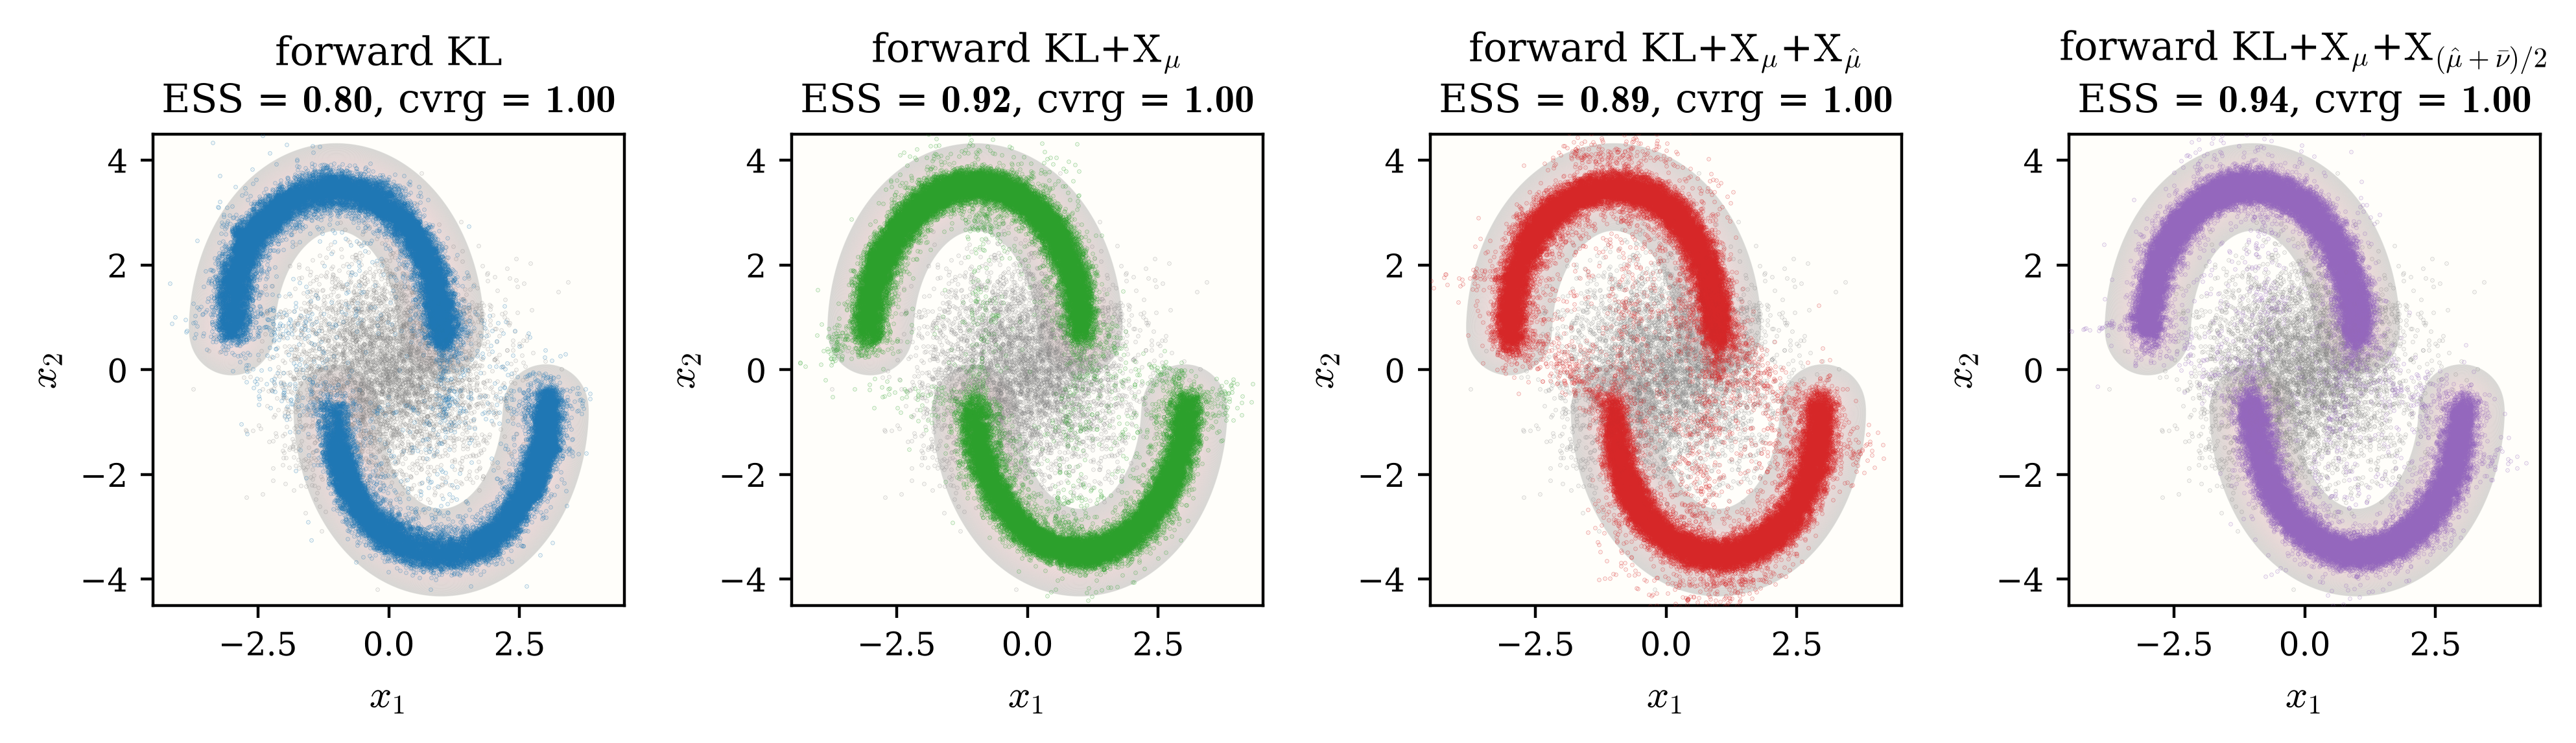
\includegraphics[width=\textwidth]{figures/2D_Benchmark/Two-Moon/samples.png}
    \caption{Two-Moon target. Columns, from left to right, are forward KL, $\KL{+}\X_\mu$, $\KL{+}\X_\mu{+}\X_{\hat\mu}$, and $\KL{+}\X_\mu{+}\X_{(\hat\mu+\bar\nu)/2}$. Each panel overlays the learned pushforward on the target energy and reports its final ESS and coverage. Gray points show the source.}
    \label{fig: two-moon}
\end{figure}

\paragraph{Two-Moon.}
The source is $\mathcal N(0,I_2)$ and both crescents lie within its reach, so all four losses attain coverage $1$. With batch size $200$, $500$ Adam steps, and learning rate $2\times10^{-3}$, the bare forward KL reaches ESS $0.8021$. Adding $\X_\mu$ raises it to $0.9157$ without additional flow evaluations, while the equal-weight mixture reaches $0.9446$ (Figure~\ref{fig: two-moon}). This benchmark isolates the accuracy role of $\X_\mu$: the pairwise term constrains the spread of the log-ratio left uncontrolled by the mean-only forward KL objective.

\begin{figure}[htb]
    \centering
    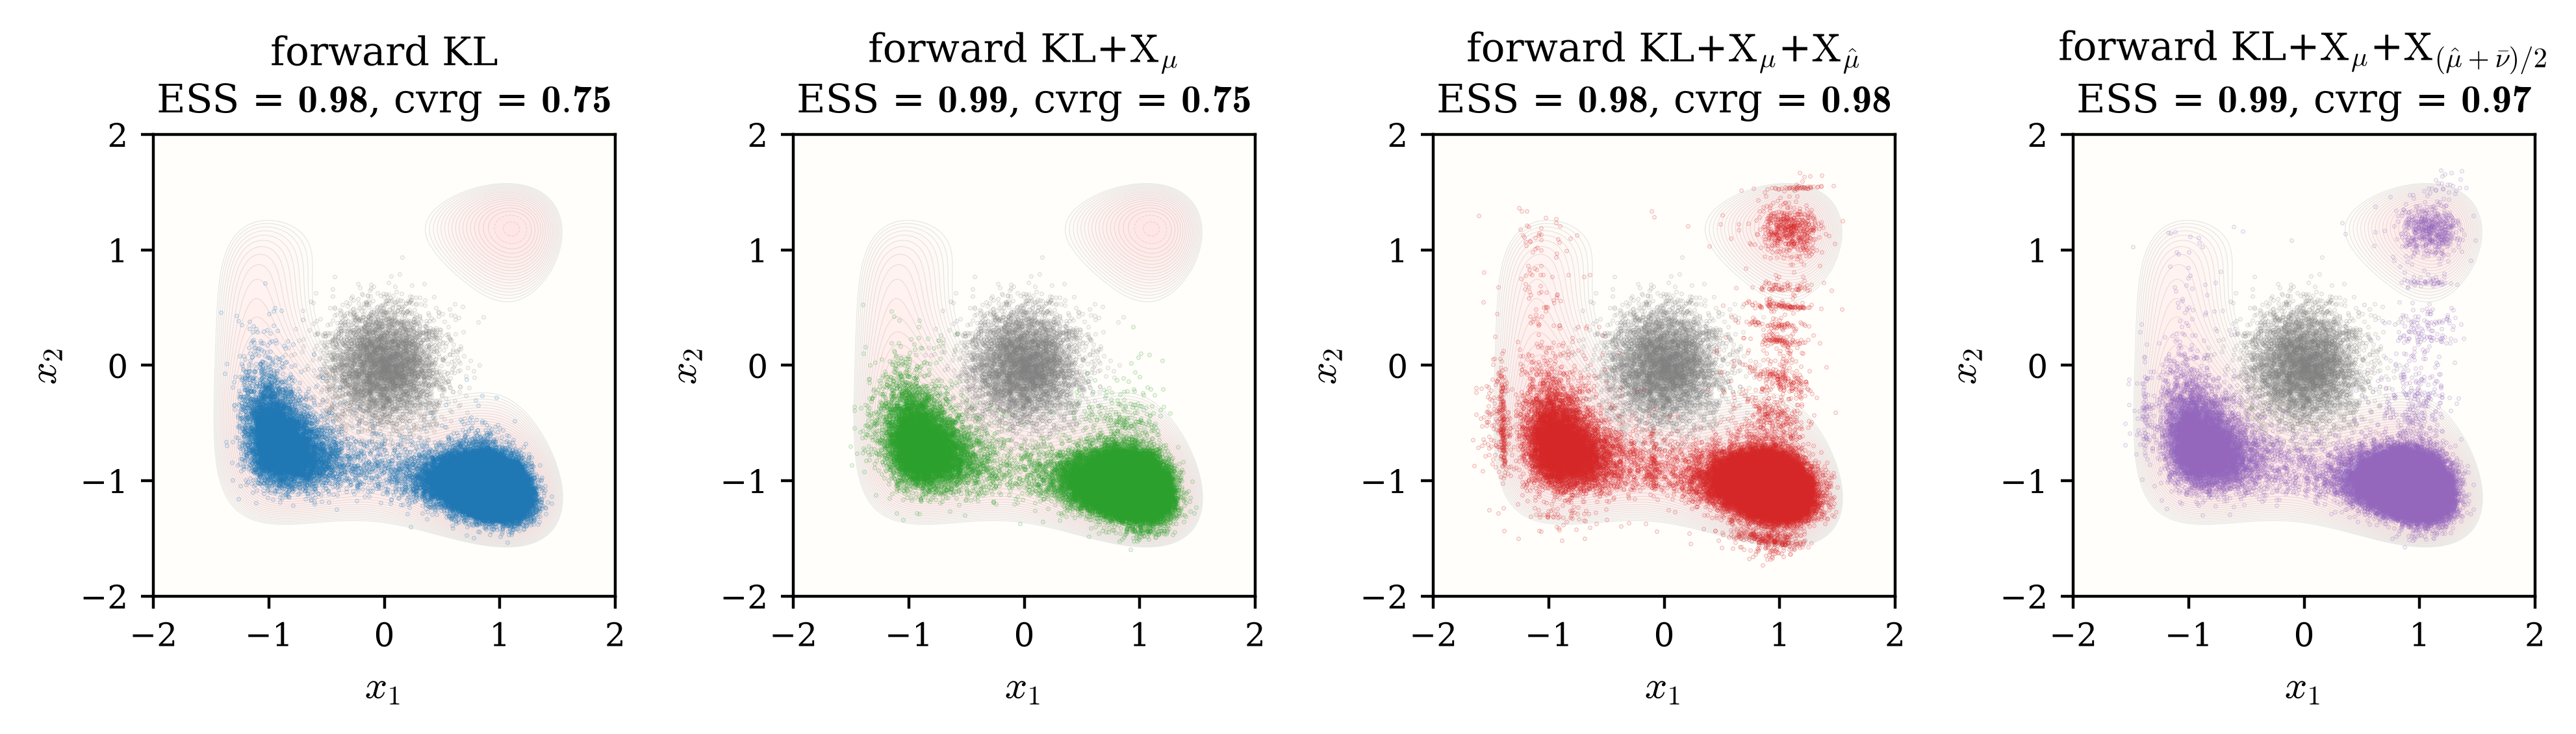
\includegraphics[width=\textwidth]{figures/2D_Benchmark/Three-Well/samples.png}
    \caption{Three-Well target. Methods and annotations are as in Figure~\ref{fig: two-moon}.}
    \label{fig: threewell}
\end{figure}

\paragraph{Three-Well.}
The source is $\mathcal N(0,0.25^2 I_2)$, narrower than the well separation and initially covering no basin. Training uses batch size $1000$, $500$ steps, and learning rate $10^{-3}$. Forward KL and $\KL{+}\X_\mu$ fill the two favored wells and report ESS $0.9830$ and $0.9933$, respectively, while their coverage remains $0.7525$. Quench and temper discovers the suppressed third well. The $\hat\mu$ and equal-weight mixtures raise coverage to $0.9763$ and $0.9660$ while retaining ESS $0.9771$ and $0.9858$ (Figure~\ref{fig: threewell}).

\begin{figure}[htb]
    \centering
    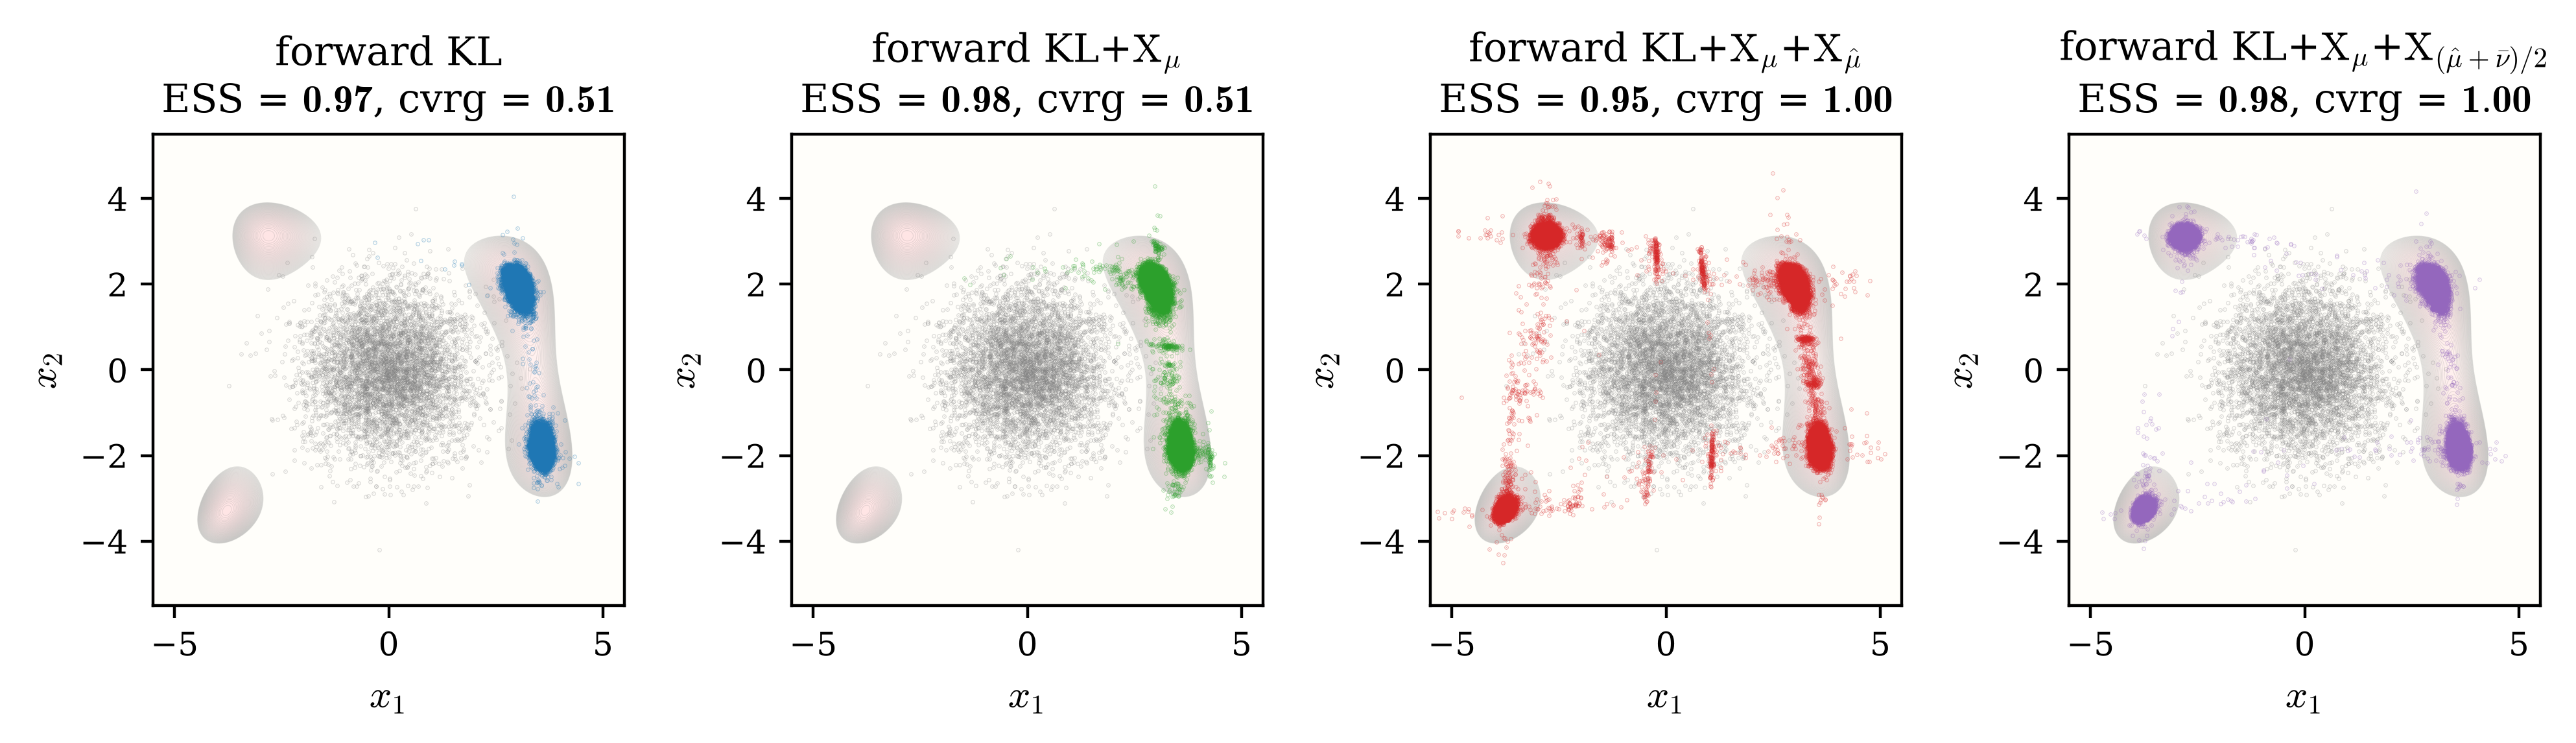
\includegraphics[width=\textwidth]{figures/2D_Benchmark/Himmelblau/samples.png}
    \caption{Himmelblau target. Methods and annotations are as in Figure~\ref{fig: two-moon}.}
    \label{fig: himmelblau}
\end{figure}

\paragraph{Himmelblau.}
The source is $\mathcal N(0,I_2)$, whereas the four wells lie at radius approximately $3$--$4$. Training uses batch size $1000$, $1000$ steps, and learning rate $10^{-3}$. Forward KL and $\KL{+}\X_\mu$ capture only two wells, giving coverage $0.5140$ despite ESS $0.9722$ and $0.9818$. Both discovery mixtures attain coverage $1$. However, the $\hat\mu$-only flow leaks thin trails of mass between wells and has ESS $0.9516$, whereas adding the $\bar\nu$ half suppresses this leakage and raises the ESS to $0.9757$ (Figure~\ref{fig: himmelblau}).

\begin{figure}[htb]
    \centering
    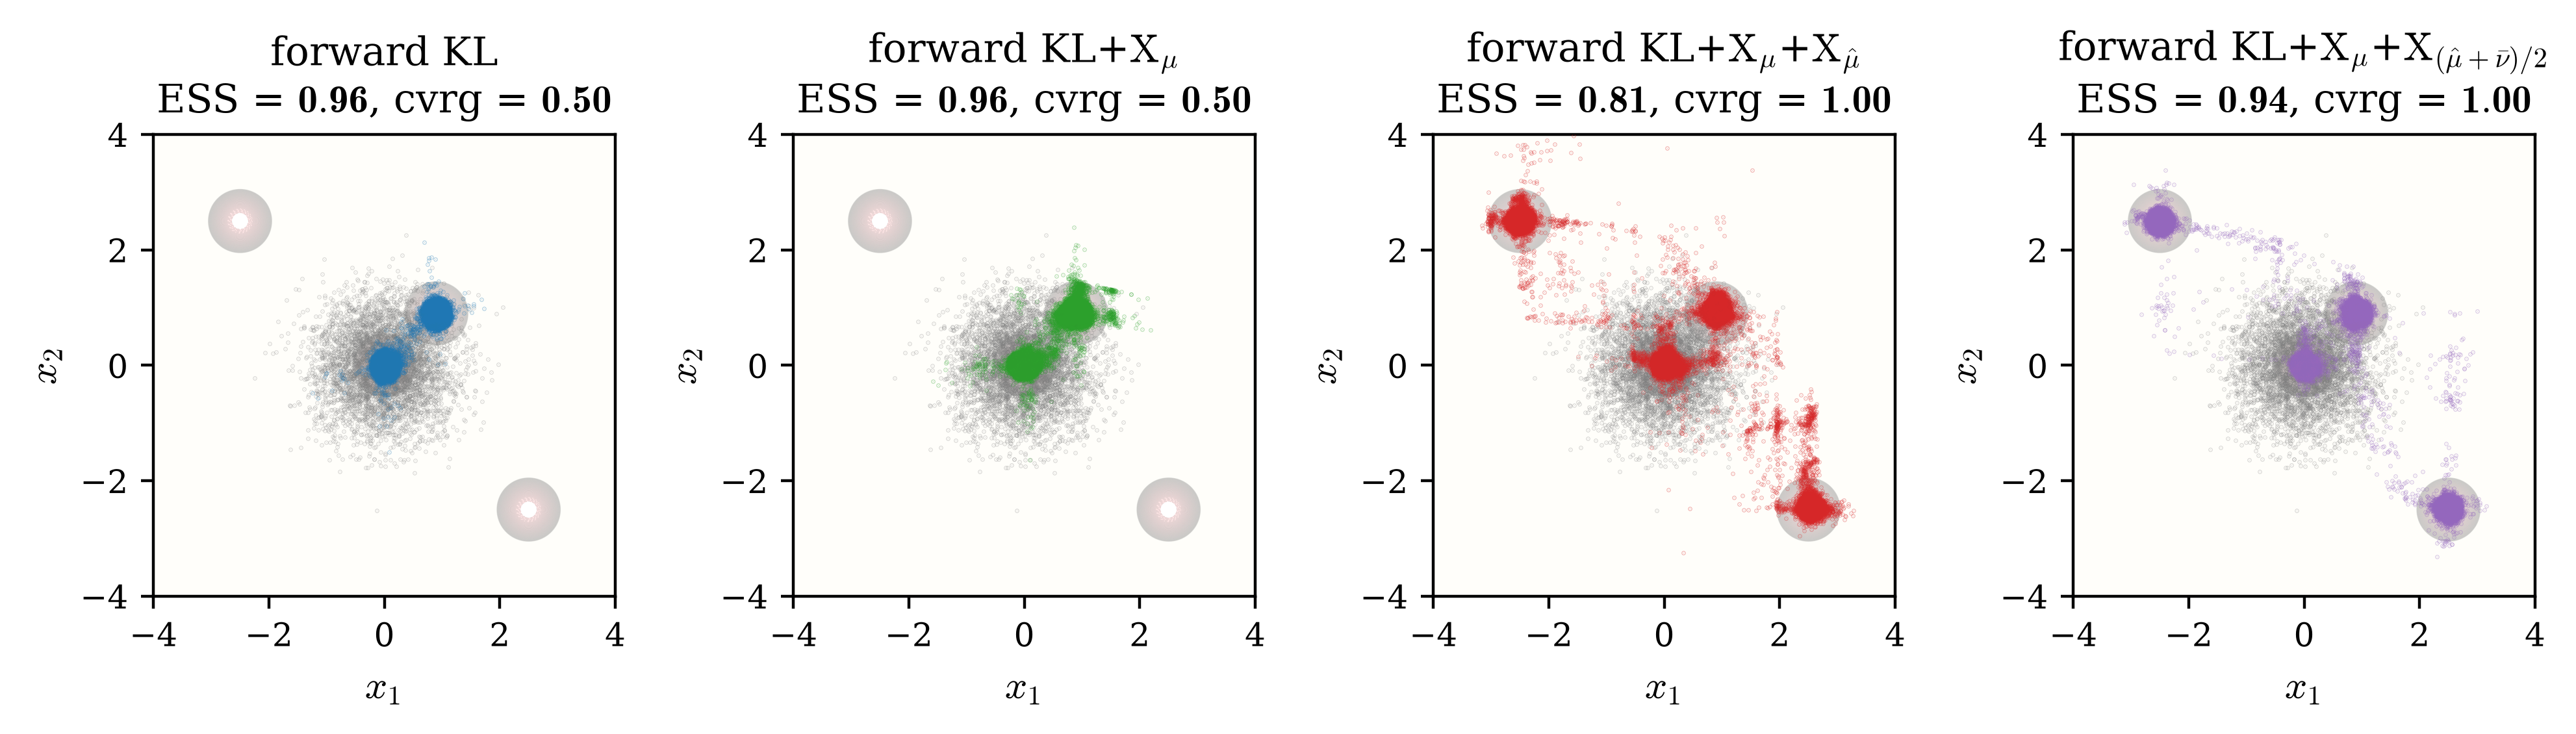
\includegraphics[width=\textwidth]{figures/2D_Benchmark/Sparse/samples.png}
    \caption{Sparse target. Methods and annotations are as in Figure~\ref{fig: two-moon}.}
    \label{fig: sparse}
\end{figure}

\paragraph{Sparse.}
The target is a four-component Gaussian mixture with component standard deviation $0.08$: two modes lie near the source center and two lie in opposite corners, more than five source standard deviations away. With source standard deviation $0.6$, batch size $1000$, $1000$ steps, and learning rate $5\times10^{-3}$, forward KL and $\KL{+}\X_\mu$ cover only the central pair. Their coverage is $0.5038$, while their ESS remains $0.9590$ and $0.9572$. The $\hat\mu$-only mixture restores coverage but pays a large leakage cost, with ESS $0.8112$. The equal-weight mixture also attains coverage $1$ and recovers most of the calibration, reaching ESS $0.9417$.

\begin{table}[htb]
    \centering
    \begin{tabular}{@{}lcccc@{}}
        \toprule
        target & KL & $\KL{+}\X_\mu$ & $\KL{+}\X_\mu{+}\X_{\hat\mu}$ & $\KL{+}\X_\mu{+}\X_{(\hat\mu+\bar\nu)/2}$ \\
        \midrule
        Two-Moon   & $0.802\,(1.000)$ & $0.916\,(1.000)$ & $0.887\,(1.000)$ & $\mathbf{0.945}\,(1.000)$ \\
        Three-Well & $0.983\,(0.753)$ & $0.993\,(0.753)$ & $0.977\,(0.976)$ & $\mathbf{0.986}\,(0.966)$ \\
        Himmelblau & $0.972\,(0.514)$ & $0.982\,(0.514)$ & $0.952\,(1.000)$ & $\mathbf{0.976}\,(1.000)$ \\
        Sparse     & $0.959\,(0.504)$ & $0.957\,(0.504)$ & $0.811\,(1.000)$ & $\mathbf{0.942}\,(1.000)$ \\
        \bottomrule
    \end{tabular}
    \caption{Final ESS, with $\kappa=5$ coverage in parentheses, on the four 2D targets. Bold marks the equal-weight mixture, which is the strongest overall setting: it attains essentially full coverage and lies within $0.02$ of the best ESS on every target.}
    \label{tab: 2d-benchmark-summary}
\end{table}

The four targets separate the objective's three mechanisms. The $\X_\mu$ term improves finite-batch accuracy when discovery is not limiting. The $\X_{\hat\mu}$ term reveals modes absent from the live AIS surrogate. The $\bar\nu$ half then penalizes the low-probability bridges introduced by aggressive discovery. The equal-weight mixture combines all three effects and is the only setting that gives essentially full coverage with near-best calibration throughout Table~\ref{tab: 2d-benchmark-summary}.

\subsection{High-dimensional product multi-well}
\label{subsec: highd}

We next isolate accuracy scaling in dimension $d=2^k$, $k=1,\ldots,8$, using
\begin{equation}
    U(\mathbf{x})=\frac12\lVert\mathbf{x}\rVert^2
    +12\sum_{i=1}^{k}\exp(-x_i^2).
    \label{eq: highd-potential}
\end{equation}
The first $k$ coordinates are symmetric double wells with minima at $\pm\sqrt{\ln 24}$ and barrier approximately $9.9$, while the remaining $d-k$ coordinates are standard Gaussian. The target therefore has exactly $2^k=d$ equal-weight modes. Multimodality occupies only a $k$-dimensional subspace, but the log-weight error accumulates across all $d$ coordinates.

All four objectives use the same identity-initialized neural spline flow on $[-4,4]^d$, with $16$ bins, $6$ transforms, and conditioner widths $(256,256)$. At every dimension, training uses batch size $250$, $2000$ Adam steps at learning rate $10^{-3}$, gradient clipping at $10^2$, and a source pool of size $10^4\,2^k$. The live target surrogate uses a single AIS hop followed by $50$ MALA steps of size $2\times10^{-3}$. Quench and temper uses a pool of size $100\,2^k$, melt scale $2$, and an Armijo L-BFGS quench with initial step $0.5$ and $200$ iterations. Final ESS is evaluated on $20000$ fresh source samples. Strict sign-pattern coverage counts a mode only if its empirical share exceeds half of the uniform share.

\begin{table}[htb]
    \centering
    \begin{tabular}{@{}lcccccccc@{}}
        \toprule
        loss $\backslash$ $d$ & 2 & 4 & 8 & 16 & 32 & 64 & 128 & 256 \\
        \midrule
        forward KL & 0.974 & 0.942 & 0.906 & 0.878 & 0.796 & 0.704 & 0.615 & 0.420 \\
        $\KL{+}\X_\mu$ & 0.997 & 0.983 & 0.958 & 0.957 & 0.909 & 0.850 & 0.744 & 0.562 \\
        $\KL{+}\X_\mu{+}\X_{\hat\mu}$ & 0.996 & 0.983 & 0.959 & 0.952 & 0.923 & 0.875 & 0.744 & 0.585 \\
        $\KL{+}\X_\mu{+}\X_{(\hat\mu+\bar\nu)/2}$ & $\mathbf{0.998}$ & $\mathbf{0.985}$ & $\mathbf{0.963}$ & $\mathbf{0.960}$ & $\mathbf{0.941}$ & $\mathbf{0.887}$ & $\mathbf{0.791}$ & $\mathbf{0.596}$ \\
        \bottomrule
    \end{tabular}
    \caption{Final ESS on the product multi-well target \eqref{eq: highd-potential}. Every loss finds all $2^k$ modes under the strict coverage threshold; bold marks the best ESS in each dimension.}
    \label{tab: highd-ess}
\end{table}

Every loss finds every mode, so ESS is meaningful here. The forward KL degrades from $0.974$ at $d=2$ to $0.420$ at $d=256$ as coordinatewise fitting errors accumulate in the log weights. Adding $\X_\mu$ improves every dimension and reaches $0.562$ at $d=256$. The equal-weight mixture is best in every column, retaining ESS $0.941$ at $d=32$ and $0.596$ at $d=256$, a factor $1.42$ above the bare forward KL.

\begin{figure}[htb]
    \centering
    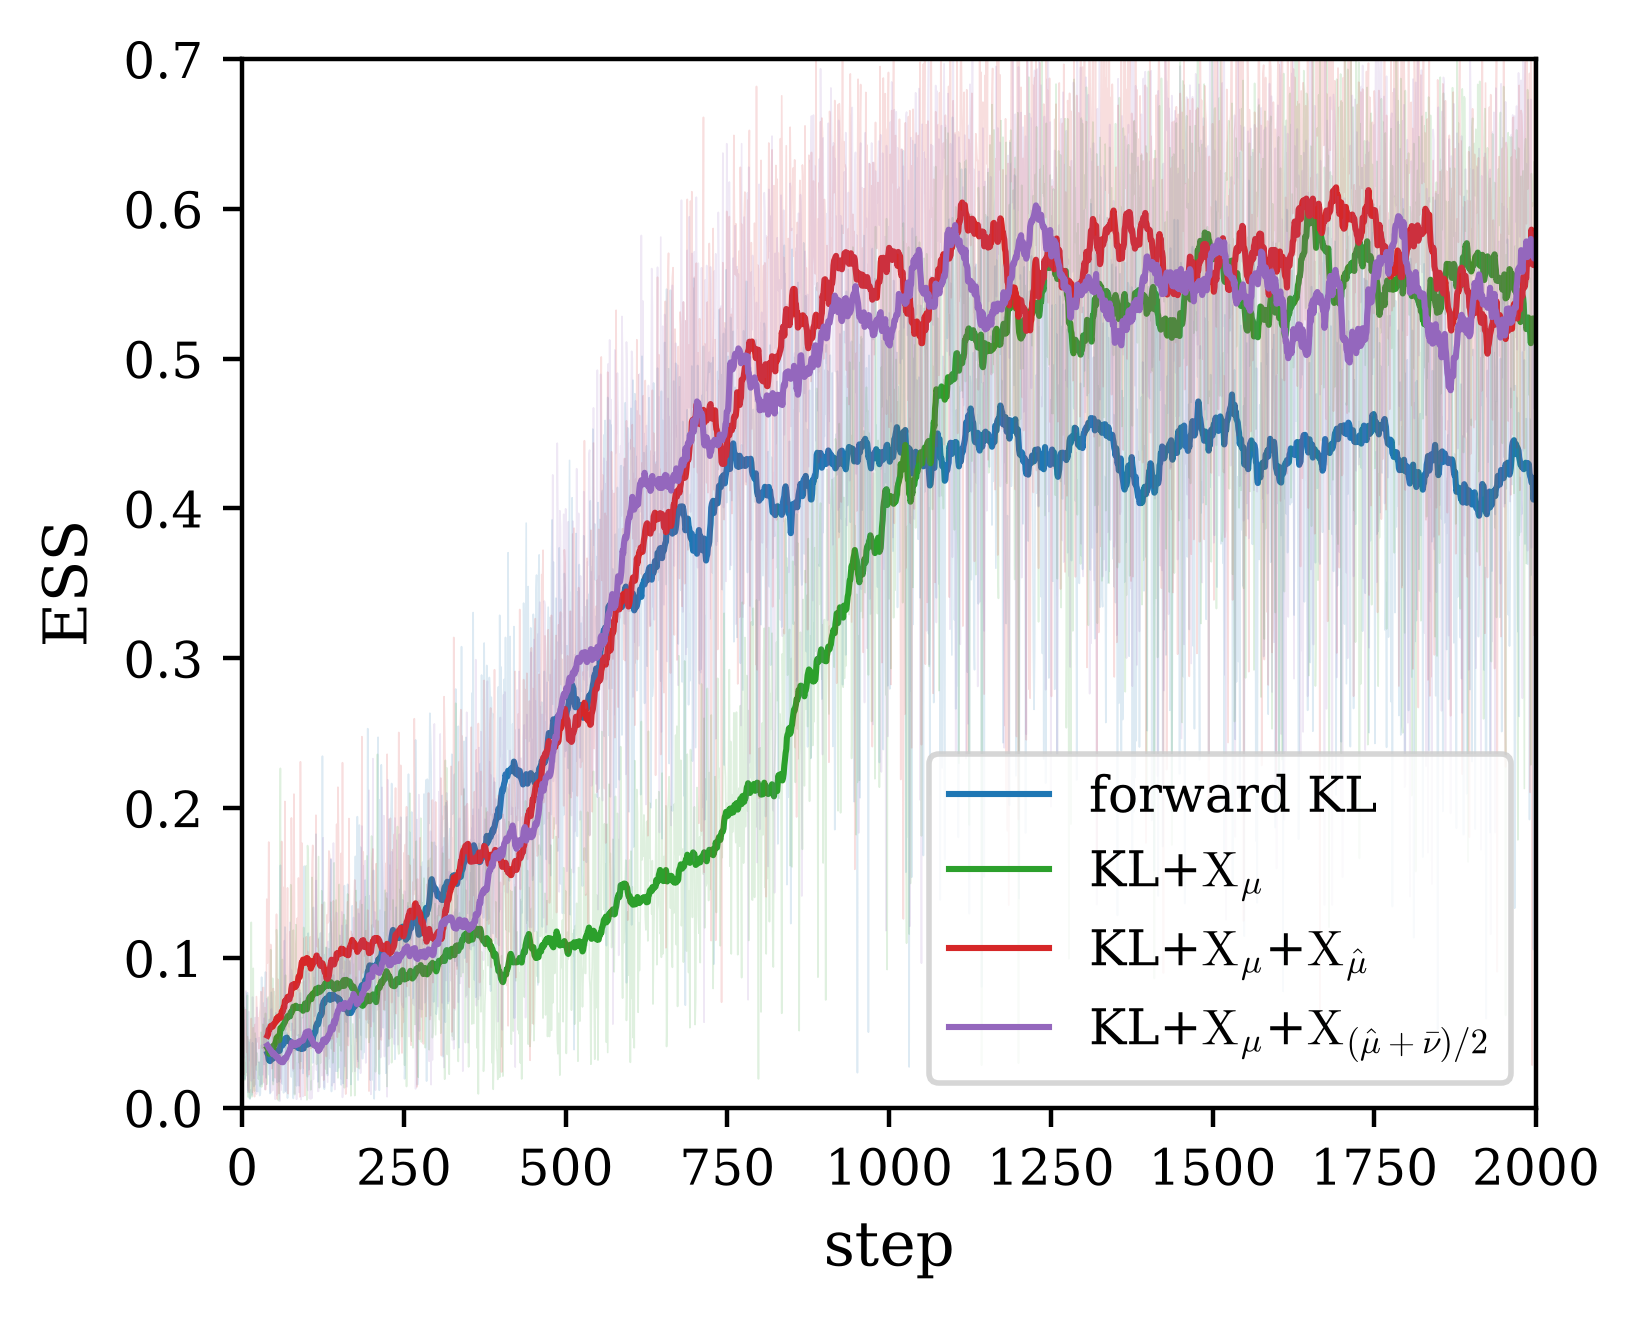
\includegraphics[width=0.4\textwidth]{figures/HD_Product/ess_k8.png}
    \caption{Per-step training ESS at $d=256$. Faint curves show raw histories and bold curves their moving averages. Forward KL rises quickly but plateaus near $0.44$; the objectives containing log-ratio variations continue improving, and the quench-and-temper mixtures finish in the highest band.}
    \label{fig: highd-ess-history}
\end{figure}

Figure~\ref{fig: highd-ess-history} separates transient speed from final accuracy. Forward KL climbs fastest during roughly the first $500$ steps but saturates early. The $\X_\mu$ objective initially trails it and then overtakes it, while the two quench-and-temper mixtures combine the fast initial climb with the highest final ESS. Thus the gain in Table~\ref{tab: highd-ess} is not obtained by sacrificing the early training regime.

\subsection{Lattice \texorpdfstring{$\phi^4$}{phi4} field theory: fake ESS at a collective barrier}
\label{subsec: phi4}

The tilted scalar $\phi^4$ theory provides a sharp fake-ESS test. On a periodic $L\times L$ lattice, with $d=L^2$ and magnetization $m(\boldsymbol\phi)=d^{-1}\sum_j\phi_j$, the action is
\begin{equation*}
U(\boldsymbol\phi)
=-0.8\sum_{\langle jl\rangle}\phi_j\phi_l
+\sum_{j=1}^{d}\left[\phi_j^2+\frac12(\phi_j^2-1)^2\right]
+\begin{cases}
0.0257\displaystyle\sum_{j=1}^{d}\phi_j, & L=6,\\
0.0144\displaystyle\sum_{j=1}^{d}\phi_j, & L=8.
\end{cases}
\end{equation*}
In the broken phase the field orders near two vacua $\pm v\mathbf 1$, separated by a collective domain-wall barrier. The positive linear term gives the two phases unequal probability, so the minority weight $p_+=\mathbb P(m>0)$ is not fixed by symmetry and must be learned.

Parallel tempering gives the references $p_+=0.125$ and $0.128$, consistent with an independent symmetry-confined MALA reweighting. Each loss is run at seeds $0,1,2$ using an identity-initialized neural spline flow on $[-3,3]^d$, with $16$ bins, $6$ transforms, and conditioner widths $(256,256)$. The source is $\mathcal N(0,0.25I_d)$, centered on the barrier. Training uses a fixed set of $10^5$ source samples, batch size $500$, $2000$ Adam steps at learning rate $10^{-3}$, and gradient clipping at $10^3$. The live surrogate uses one AIS hop and $50$ MALA steps of size $2\times10^{-3}$. Quench and temper uses $2000$ particles, melt scale $2$, and an Armijo L-BFGS quench with initial step $0.1$ and $200$ iterations.

\begin{table}[htb]
    \centering
    \begin{tabular}{@{}l cc cc@{}}
        \toprule
        & \multicolumn{2}{c}{$L=6$ ($d=36$)} & \multicolumn{2}{c}{$L=8$ ($d=64$)} \\
        \cmidrule(lr){2-3}\cmidrule(lr){4-5}
        & ESS & $p_+$ & ESS & $p_+$ \\
        \midrule
        forward KL
        & $0.78/0.82/0.82$ & $1/1/0$
        & $0.67/0.68/0.67$ & $1/0/1$ \\
        $\KL{+}\X_\mu$
        & $0.93/0.93/0.94$ & $1/1/0$
        & $0.81/0.82/0.82$ & $1/0/0$ \\
        $\KL{+}\X_\mu{+}\X_{\hat\mu}$
        & $0.88/0.87/0.87$ & $0.127/0.128/0.126$
        & $0.62/0.61/0.63$ & $0.127/0.126/0.124$ \\
        $\KL{+}\X_\mu{+}\X_{(\hat\mu+\bar\nu)/2}$
        & $\mathbf{0.90/0.89/0.88}$ & $0.128/0.129/0.128$
        & $\mathbf{0.67/0.68/0.71}$ & $0.130/0.129/0.130$ \\
        \midrule
        PT reference & --- & $0.125$ & --- & $0.128$ \\
        \bottomrule
    \end{tabular}
    \caption{Final ESS and reweighted minority-phase weight $p_+$ for three seeds on the tilted $\phi^4$ lattice. Integer values $0$ and $1$ indicate collapse onto one vacuum. Bold marks the highest ESS among the objectives that recover both phases.}
    \label{tab: phi4}
\end{table}

Forward KL and $\KL{+}\X_\mu$ collapse at every size and seed. Because the AIS chain starts from the flow pushforward and cannot cross the collective barrier, the second vacuum remains absent and reweighting gives $p_+=0$ or $1$. Nevertheless, $\KL{+}\X_\mu$ has the highest ESS at both sizes: sharpening the captured vacuum improves calibration on the reached support while making the global failure no less severe.

\begin{figure}[htb]
    \centering
    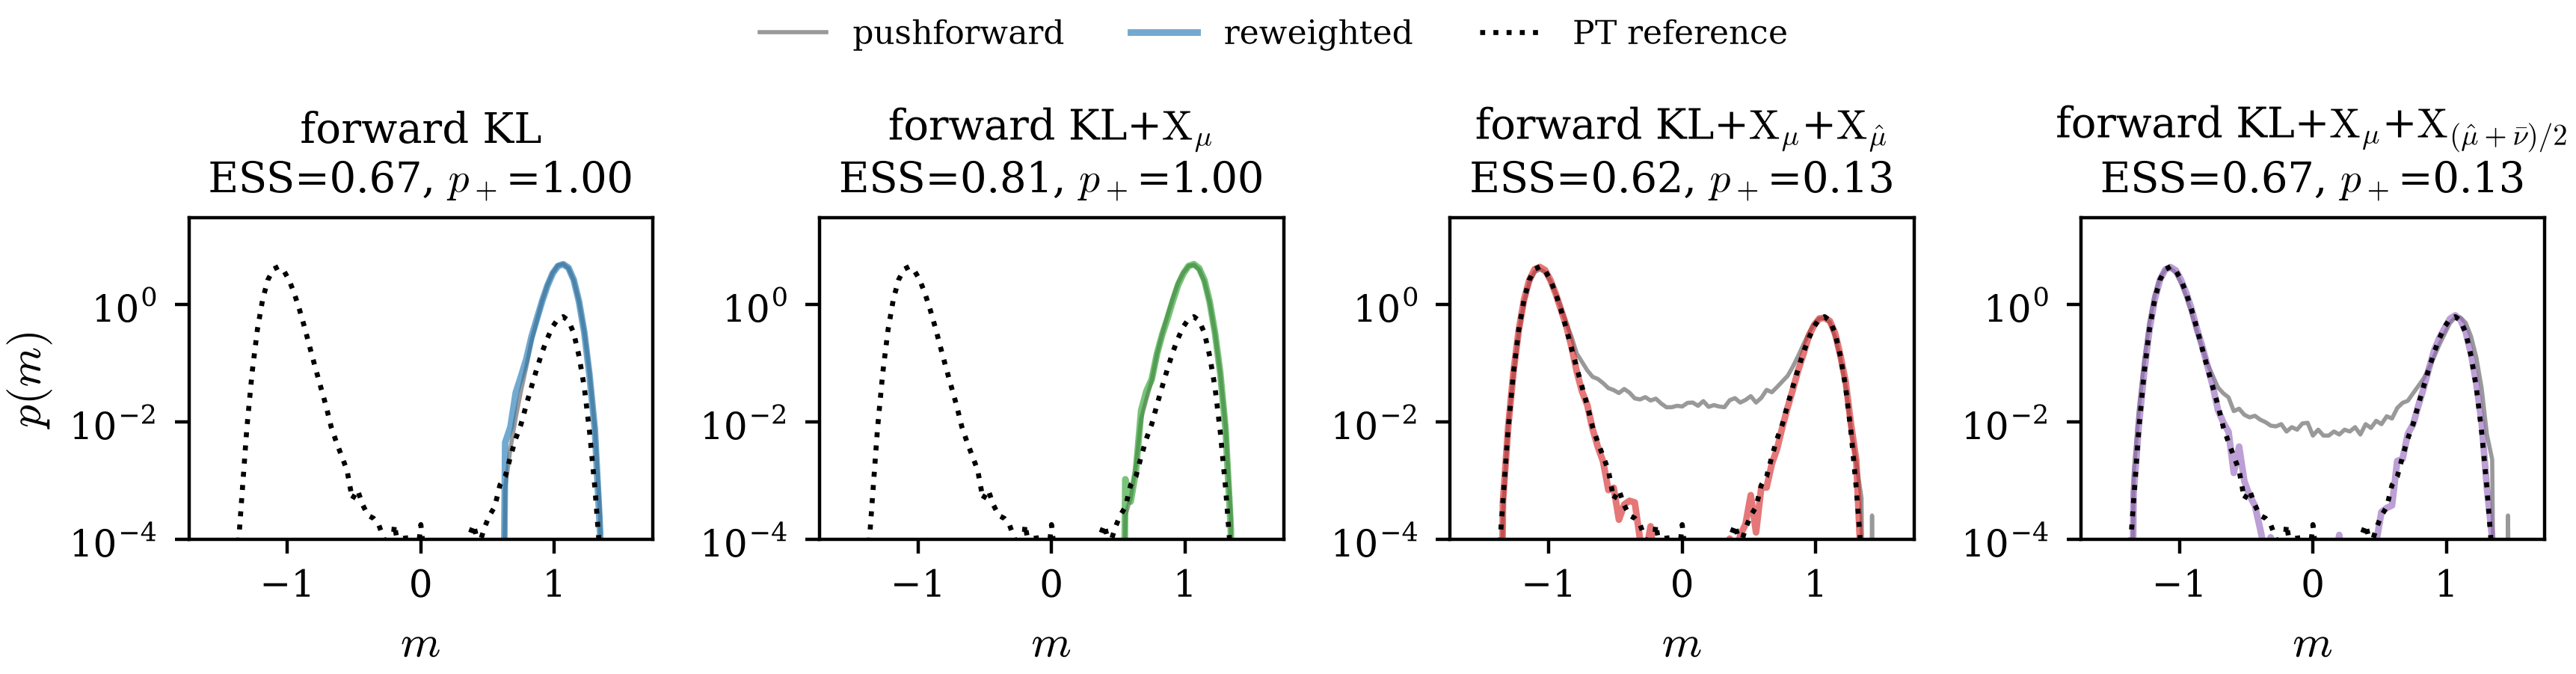
\includegraphics[width=\textwidth]{figures/Lattice_Phi4/L8/fig_methods.png}
    \caption{Magnetization density on the $L=8$ lattice at seed $0$. Each panel shows the pushforward density (gray), the reweighted density (color), and the parallel-tempering reference (dotted); the title reports ESS and the reweighted $p_+$.}
    \label{fig: phi4-methods}
\end{figure}

Both quench-and-temper objectives populate both vacua at every seed. Their recovered $p_+$ lies between $0.124$ and $0.130$, within $0.004$ of the corresponding reference. This recovery has an unavoidable ESS cost: a diffeomorphism maps the connected Gaussian source to a connected pushforward, so covering both vacua forces a low-weight bridge across the suppressed inter-phase region. At $L=8$, the equal-weight mixture recovers part of this cost, with ESS $0.67$--$0.71$ rather than $0.61$--$0.63$ for the $\hat\mu$-only objective. The $\bar\nu$ component penalizes precisely the leaked bridge mass while preserving discovery.

\subsection{Boltzmann generator on \texorpdfstring{$p$}{p}-state clock model}
\label{subsec: clock}

The preceding benchmarks use a single flow. We now test the full annealed construction on the $p=6$ clock model on a periodic $8\times8$ lattice,
\begin{equation}
U(\boldsymbol\theta)
=-\sum_{\langle jl\rangle}\cos(\theta_j-\theta_l)
-\frac12\sum_{j=1}^{d}\cos(6\theta_j),
\qquad \boldsymbol\theta\in[-\pi,\pi)^{d},\quad d=64,
\label{eq: clock-potential}
\end{equation}
where $\langle jl\rangle$ runs over nearest-neighbor pairs. The source is uniform on the torus and the bridge is $U_t=tU$. At low temperature, the target separates into six symmetry-related clock sectors.

Each stage uses an identity-initialized neural circular spline flow with $16$ bins, $6$ autoregressive transforms, and conditioner widths $(256,256)$. The validation set contains $4\times10^5$ particles and the SMC and quench-and-temper pools each contain $10^5$ particles. Every stage uses $3000$ Adam steps at learning rate $10^{-3}$, a four-stage training AIS surrogate with $100$ MALA steps of size $10^{-3}$, energy clipping at $10^3$, and gradient clipping at $10^2$. We test batch sizes $B=2000,1000,500,250,125$.

The comparison is schedule-matched. Forward KL first constructs an adaptive ladder using SMC preselection and an ESS acceptance gate. The loss $\KL{+}\X_\mu{+}\X_{(\hat\mu+\bar\nu)/2}$ is then trained on the identical accepted values of $t$, without a second gate. Hence the two methods see the same bridge increments within each batch-size pair. Every configuration is a single run, so individual stage values carry single-run fluctuation.

The principal metric is the validation ESS of each accepted increment. We define
\[
\text{propagation factor}\quad F:=\prod_k \mathrm{ESS}_k^{-1}
\]
estimates the factor by which staged reweighting enlarges Monte Carlo error across the full ladder. Smaller $F$ is better. Table~\ref{tab: clock-summary} reports every accepted stage and the resulting $F$.

\begin{table}[htb]
    \centering
    \setlength{\tabcolsep}{2.2pt}
    \begin{tabular}{@{}lccccccccccc@{}}
        \toprule
        stage $k$ & 1 & 2 & 3 & 4 & 5 & 6 & 7 & 8 & 9 & 10 & $F$ \\
        \midrule
        $t_k$ ($B=2000$) & 0.250 & 0.495 & 0.663 & 0.779 & 0.887 & 1.000 & $\times$ & $\times$ & $\times$ & $\times$ &  \\
        forward KL & 0.752 & 0.572 & 0.499 & 0.506 & 0.527 & 0.630 & --- & --- & --- & --- & 27.7 \\
        $\KL{+}\X_\mu{+}\X_{(\hat\mu+\bar\nu)/2}$ & $\mathbf{0.919}$ & $\mathbf{0.767}$ & $\mathbf{0.643}$ & $\mathbf{0.587}$ & $\mathbf{0.578}$ & $\mathbf{0.664}$ & --- & --- & --- & --- & $\mathbf{9.8}$ \\
        \midrule
        $t_k$ ($B=1000$) & 0.250 & 0.495 & 0.663 & 0.779 & 0.887 & 1.000 & $\times$ & $\times$ & $\times$ & $\times$ &  \\
        forward KL & 0.678 & 0.492 & 0.419 & 0.450 & 0.487 & 0.585 & --- & --- & --- & --- & 55.7 \\
        $\KL{+}\X_\mu{+}\X_{(\hat\mu+\bar\nu)/2}$ & $\mathbf{0.863}$ & $\mathbf{0.659}$ & $\mathbf{0.539}$ & $\mathbf{0.507}$ & $\mathbf{0.522}$ & $\mathbf{0.610}$ & --- & --- & --- & --- & $\mathbf{20.2}$ \\
        \midrule
        $t_k$ ($B=500$) & 0.250 & 0.421 & 0.590 & 0.705 & 0.818 & 0.945 & 1.000 & $\times$ & $\times$ & $\times$ & \\
        forward KL & 0.580 & 0.556 & 0.428 & 0.464 & 0.401 & 0.412 & 0.784 & --- & --- & --- & 120.9 \\
        $\KL{+}\X_\mu{+}\X_{(\hat\mu+\bar\nu)/2}$ & $\mathbf{0.778}$ & $\mathbf{0.705}$ & $\mathbf{0.530}$ & $\mathbf{0.535}$ & $\mathbf{0.430}$ & $\mathbf{0.416}$ & 0.784 & --- & --- & --- & $\mathbf{45.7}$ \\
        \midrule
        $t_k$ ($B=250$) & 0.250 & 0.421 & 0.539 & 0.654 & 0.734 & 0.811 & 0.887 & 1.000 & $\times$ & $\times$ & \\
        forward KL & 0.470 & 0.464 & 0.512 & 0.428 & 0.522 & 0.493 & 0.534 & 0.476 & --- & --- & 319.6 \\
        $\KL{+}\X_\mu{+}\X_{(\hat\mu+\bar\nu)/2}$ & $\mathbf{0.662}$ & $\mathbf{0.603}$ & $\mathbf{0.625}$ & $\mathbf{0.503}$ & $\mathbf{0.584}$ & $\mathbf{0.540}$ & $\mathbf{0.564}$ & 0.476 & --- & --- & $\mathbf{94.1}$ \\
        \midrule
        $t_k$ ($B=125$) & 0.175 & 0.295 & 0.413 & 0.528 & 0.607 & 0.685 & 0.761 & 0.835 & 0.908 & 1.000 & \\
        forward KL & 0.455 & 0.506 & 0.472 & 0.434 & 0.533 & 0.514 & $\mathbf{0.514}$ & $\mathbf{0.547}$ & $\mathbf{0.601}$ & $\mathbf{0.515}$ & 891.1 \\
        $\KL{+}\X_\mu{+}\X_{(\hat\mu+\bar\nu)/2}$ & $\mathbf{0.656}$ & $\mathbf{0.698}$ & $\mathbf{0.637}$ & $\mathbf{0.553}$ & $\mathbf{0.634}$ & $\mathbf{0.559}$ & 0.509 & 0.501 & 0.559 & 0.496 & $\mathbf{246.3}$ \\
        \bottomrule
    \end{tabular}
    \caption{Validation ESS on every accepted stage of the schedule-matched clock-model comparison between forward KL and $\KL{+}\X_\mu{+}\X_{(\hat\mu+\bar\nu)/2}$. Within each batch-size block, both losses traverse the same ladder. The final column is $F=\prod_k\mathrm{ESS}_k^{-1}$; bold marks the better loss on each stage and the smaller $F$.}
    \label{tab: clock-summary}
    \label{tab: clock-ladder}
\end{table}

The loss $\KL{+}\X_\mu{+}\X_{(\hat\mu+\bar\nu)/2}$ raises the geometric mean stage ESS by $0.07$--$0.11$ at every batch size and reduces $F$ by a factor between $2.6$ and $3.6$. The advantage therefore persists at the largest batch $B=2000$, where $F$ decreases from $27.7$ to $9.8$. As the batch shrinks, both ladders lengthen, from $6$ stages at $B=2000$ to $10$ at $B=125$, and error propagation grows sharply.

The improvement is concentrated on early and middle stages. There the bridge deformation is large but smooth, so fitting accuracy is the binding constraint. Near $t=1$, the six sectors separate and the problem shifts from fitting within sectors to transporting their relative mass. Reweighting, common to both losses, performs that redistribution. At $B=125$, forward KL is slightly better on the final four stages, where quench-and-temper discovers sectors but does not assign their exact weights. This is the main limitation observed in the ladder experiment. By $B\Ge 1000$, $\KL{+}\X_\mu{+}\X_{(\hat\mu+\bar\nu)/2}$ again leads on every stage.

\begin{figure}[htb]
    \centering
    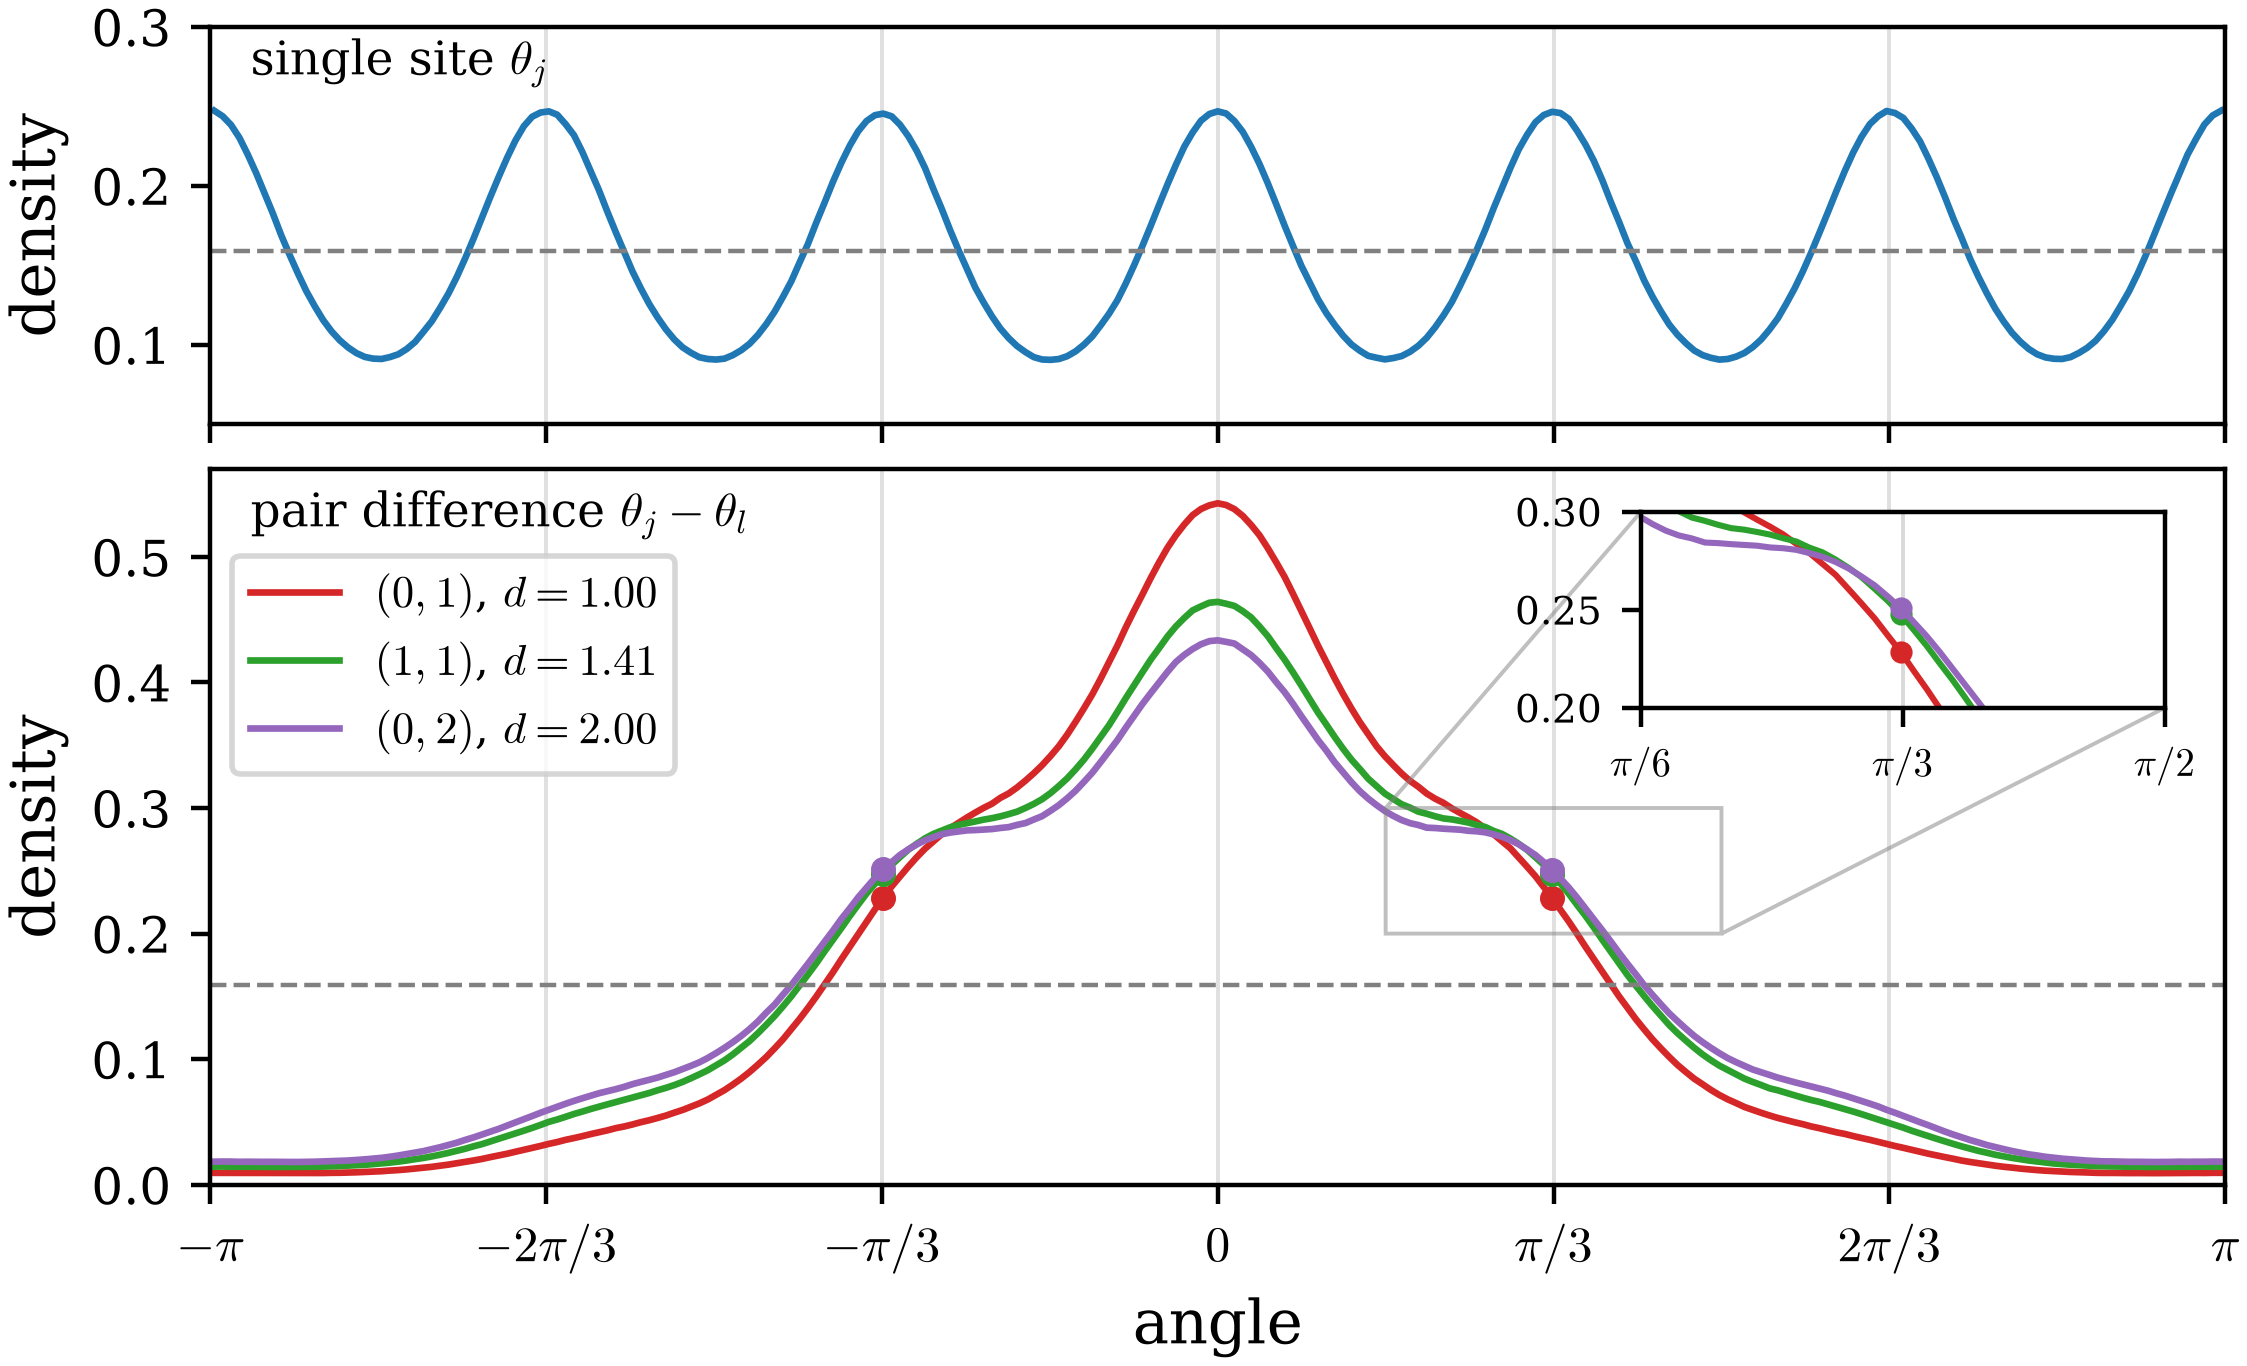
\includegraphics[width=0.7\textwidth]{figures/Lattice_Clock/clock_marginals.png}
    \caption{Angle densities from $2\times10^6$ fresh samples advanced through the trained $B=2000$ $\KL{+}\X_\mu{+}\X_{(\hat\mu+\bar\nu)/2}$ ladder by map, reweighting, resampling, and MALA. The single-site marginal peaks at the six clock angles. Pair-difference densities at increasing lattice separation retain an alignment peak at zero while transferring mass toward neighboring clock wells and the tails.}
    \label{fig: clock-marginals}
\end{figure}

All six sectors are found at every batch size. To test whether staged resampling preserves their symmetry, we rebuild fresh samples through the trained $B=2000$ ladders at sizes $N=10^4\,2^k$, $k=0,\ldots,8$, using equal total work of $2.56\times10^6$ particles per row. We define
\[
\operatorname{occupancy\ bias}:=\frac16\sum_{s=0}^{5}\left|p_s-\frac16\right|.
\]

\begin{figure}[htb]
    \centering
    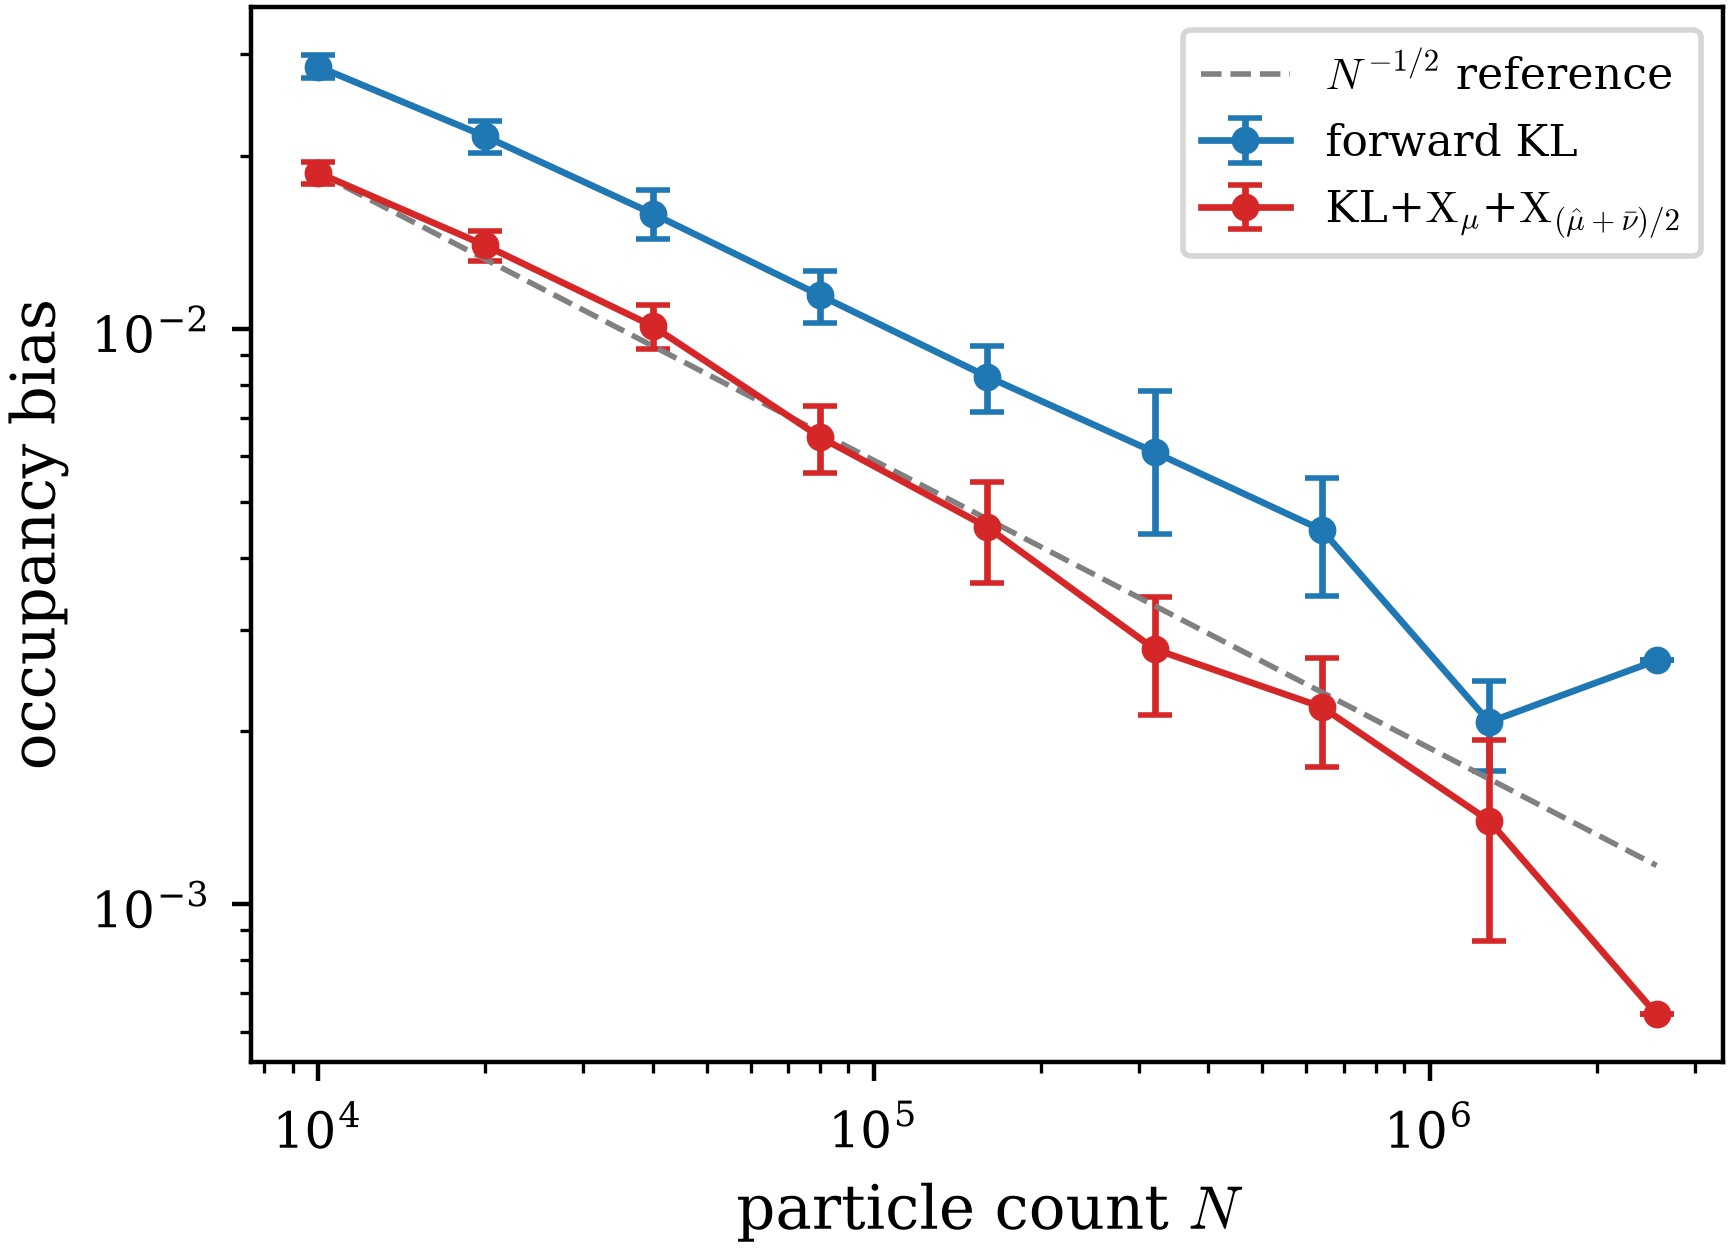
\includegraphics[width=0.55\textwidth]{figures/Lattice_Clock/occupancy_bias_B2000.png}
    \caption{Clock-sector occupancy bias versus fresh rebuild size. Error bars are $\pm2$ standard errors, and the dashed line is an $N^{-1/2}$ reference anchored at the smallest $\KL{+}\X_\mu{+}\X_{(\hat\mu+\bar\nu)/2}$ point. Each curve replays one trained ladder, so the cross-loss comparison retains the single-run qualification.}
    \label{fig: clock-occupancy}
\end{figure}

Both losses approach the Monte Carlo scaling rate: fitted log--log slopes are $-0.474$ for forward KL and $-0.584$ for $\KL{+}\X_\mu{+}\X_{(\hat\mu+\bar\nu)/2}$. The $\KL{+}\X_\mu{+}\X_{(\hat\mu+\bar\nu)/2}$ ladder has lower occupancy bias at every tested size and reaches $6.4\times10^{-4}$ at $N=2.56\times10^6$. The largest-$N$ point of each curve is a single rebuild and therefore influences the fitted slopes. Together with Table~\ref{tab: clock-summary}, this shows that the per-stage ESS improvement survives composition without hiding a sector imbalance, while the late-stage reversal remains confined to the smallest-batch corner.
% ===================== Section 6: molecular (FULL verbatim) =====================
\section{Boltzmann generators on molecular potential energies}
\label{sec: molecular}

Each model problem of the previous section isolates one failure mode of forward KL training
on a smooth target: the 2D benchmarks, the high-dimensional multi-well, the lattice $\phi^4$ theory, and the $p$-state clock model.
The application that motivates a Boltzmann generator is a molecule. A molecular target
exercises the whole pipeline at once. This section applies the adaptive-temperature, X-regularized generator
of the previous section to three molecules of increasing difficulty in full internal coordinates,
$d = 36$ to $60$, on a single consumer GPU. It has five parts: the motivation and the two
difficulties that make a molecular potential hard (Section~\ref{sec: mol-background}); \emph{sharpening}, the simplification that makes the framework tractable on a singular target (Section~\ref{sec: mol-sharpening}); the
molecule-specific engineering it requires (Section~\ref{sec: mol-engineering}); the numerical results on
glycerol, diethanolamine, and alanine dipeptide (Section~\ref{sec: mol-results}); and the limitations of the
molecular study (Section~\ref{sec: mol-limitations}).

\subsection{Motivation and background}
\label{sec: mol-background}

Concretely, the target is the equilibrium (Boltzmann) distribution
$\mu \propto e^{-U}$ of a molecular potential, with $U$ its dimensionless reduced form. Its samples are the conformers that set binding
affinities, reaction rates, and free energies in computational chemistry and drug design
\citep{noe2019boltzmann}. The targets studied so far are smooth by design; a molecular potential is not. Drawing \emph{independent} samples from
$\mu$ is the central computational problem. MD and MCMC mix slowly across
the high torsion barriers that separate conformers. A trained flow that emits independent conformers with a
tractable density supports the exact importance-sampling pipeline of the previous sections, and this payoff
justifies the training cost.

We take the potential energy to be the Amber molecular-mechanics force field \citep{cornell1995amber}, the
standard classical model. Its raw force-field energy $U_{\mathrm{FF}}(x)$ in kJ/mol sums bonded terms, harmonic bonds and angles and
periodic torsions, and nonbonded Lennard-Jones and Coulomb terms,
\begin{equation}
    U_{\mathrm{FF}}(x) = \!\!\sum_{\text{bonds}}\!\! k_b (r-r_0)^2 + \!\!\sum_{\text{angles}}\!\! k_\theta (\theta-\theta_0)^2
    + \!\!\sum_{\text{torsions}}\!\! \frac{V_n}{2}\big[1+\cos(n\phi-\gamma)\big]
    + \sum_{i<j}\!\bigg[ 4\epsilon_{ij}\bigg(\frac{\sigma_{ij}^{12}}{r_{ij}^{12}} - \frac{\sigma_{ij}^{6}}{r_{ij}^{6}}\bigg) + \frac{q_i q_j}{r_{ij}} \bigg],
    \label{eq: amber}
\end{equation}
the last sum running over nonbonded atom pairs, with charges in units that absorb the Coulomb constant. The
Boltzmann distribution at temperature $T$ is $\mu \propto e^{-U}$ in the dimensionless reduced potential
\begin{equation*}
    U(x) = \frac{1}{k_B T} U_{\mathrm{FF}}(x),
\end{equation*}
with $k_B$ the Boltzmann constant. We evaluate $U_{\mathrm{FF}}$ for the \emph{isolated
molecule in vacuum}, with no solvent and no nonbonded cutoff. Section~\ref{sec: mol-limitations} discusses
this and two further simplifications of the molecular study.

We work in \emph{whitened internal coordinates} \citep{noe2019boltzmann}. The six rigid-body degrees of
freedom, global translation and rotation, leave $U$ unchanged. We drop them and describe the shape by
bond lengths, bond angles, and torsions. A z-matrix gives a smooth, invertible map $x \mapsto \xi \in
\mathbb R^{d}$ with $d = 3N - 6$ for an $N$-atom molecule and a tractable volume Jacobian. Bonds and angles are stiff and near-Gaussian
about their equilibria, so each is standardized to unit variance; torsions stay periodic on $[-\pi,\pi)$. The
source $\mu_0 \propto e^{-U_0}$ is then a product base, standard normal on the bond/angle
directions and uniform on the torsions. The target, pulled back through the change of variables, is
\begin{equation*}
    \mu(\xi) \propto \exp\!\big(\!-U(x(\xi))\big)\big|\det\big(\partial x/\partial \xi\big)\big|,
\end{equation*}
so $U_0$ and $U$ as functions of $\xi$ already absorb the change-of-variables log-Jacobian. This
makes the target tractable for a flow. The rigid-body symmetries and the stiff, correlated
bond/angle vibrations are factored out, leaving the combinatorially multimodal torsional landscape, the
conformers, as the structure the diffeomorphism must transport.

Two features make \eqref{eq: amber} harder than a smooth model target, and they compound. First,
the dimension grows with the molecule ($d = 36$ to $60$ here), and the conformer landscape is
\emph{combinatorially multimodal}: every rotatable torsion is multi-well (gauche$^{\pm}$/trans), so the joint
over several torsions has dozens of basins the flow must discover. Second, the
Lennard-Jones $r^{-12}$ repulsion makes $U$ \emph{singular}: as any pair distance $r_{ij} \to 0$ the energy
diverges, so the target has a hard, near-singular clash boundary that a smooth diffeomorphism cannot represent
without enormous Jacobians. Neither difficulty is decisive alone, since high-dimensional smooth targets
and low-dimensional singular ones are both routine. Together they are worse than either: the
singular clash core sits \emph{inside} the high-dimensional multimodal landscape, and a single flow asked to
discover modes \emph{and} resolve the singularity at once trains badly at both. This compounding,
absent from every model problem of the previous section, is what the rest of this section
addresses. On alanine dipeptide ($d = 60$) below it is decisive: the clash core, not the torsion profile,
becomes the binding constraint.

\subsection{Sharpening: the core simplification}
\label{sec: mol-sharpening}

Sharpening keeps the singular part out of the flow, by annealing a second index the flow never sees. Annealing runs from the source $U_0$ of Section~\ref{sec: mol-background} to the target, for which we write the alias $U_1 = U$. A \emph{regularization} index $s \in [0,1]$ defines a soft-core target $U_{1,s}$ by taming the $r \to 0$ clash of the raw energy $U_{\mathrm{FF}}$ \eqref{eq: amber} before its reduction by $k_B T$. Two soft-core parameters act on $U_{\mathrm{FF}}$: an energy cap $e_{\mathrm{cap}}$ (kJ/mol) that log-compresses the energy above its threshold to $e_{\mathrm{cap}} + a \log(1 + (U_{\mathrm{FF}} - e_{\mathrm{cap}})/a)$ with fixed scale $a = 50$ kJ/mol, a $C^1$ wall of finite height and gradient (a hard clamp would zero the escape force); and a distance floor $r_{\mathrm{floor}}$ (nm) that replaces each nonbonded pair distance by $\max(r_{ij}, r_{\mathrm{floor}})$, removing the $r_{ij}^{-12}$ pole. Writing $U_{\mathrm{FF}}\big|_{e_{\mathrm{cap}}, r_{\mathrm{floor}}}$ for the regularized energy, the reduced soft-core target is
\begin{equation}
    U_{1,s} = \frac{1}{k_B T} U_{\mathrm{FF}}\big|_{e_{\mathrm{cap}}(s), r_{\mathrm{floor}}(s)},
    \label{eq: softcore}
\end{equation}
with the cap threshold $e_{\mathrm{cap}}(s)$ and floor $r_{\mathrm{floor}}(s)$ annealed from soft ($s=0$) to sharp ($s=1$) on a geometric or arithmetic schedule,
\begin{equation*}
    e_{\mathrm{cap}}(s) = e_{\min}(e_{\max}/e_{\min})^{s} \ \text{ or }\ e_{\min} + (e_{\max}-e_{\min})s, \qquad
    r_{\mathrm{floor}}(s) = r_{\max} + (r_{\min}-r_{\max})s,
\end{equation*}
between a low cap $e_{\min}$ and high cap $e_{\max}$, and a loose floor $r_{\max}$ and the physical floor $r_{\min}$. Both controls act only on the high-energy clash region, inactive on the equilibrium basins where $U_{\mathrm{FF}} \Le e_{\mathrm{cap}}$ and $r_{ij} > r_{\mathrm{floor}}$, so $U_{1,1} = U_1$ there and $U_{0,s} = U_0$ for all $s$. The bridge potential carries both indices,
\begin{equation*}
    U_{t,s} = (1-t)U_0 + t U_{1,s},
\end{equation*}
and the whole run is a single anneal from the soft source $U_{0,0}$ to the sharp target $U_{1,1}$, the regularization reaching the temperature at every accepted stage, $s_k = t_k$. The two indices coincide only at the accepted nodes. Within a stage they differ: $t$ first advances to $t_k$ while $s$ lags at $s_{k-1}$, then $s$ catches up to $s_k$, as described next.

The change from Algorithm~\ref{alg: boltzmann} is one extra, flow-free step per stage. Algorithm~\ref{alg: boltzmann} advances the single temperature index $t$ on the bridge $U_{t_k}$; with sharpening each stage advances the pair $(t,s)$ in two sub-steps,
\begin{equation*}
    \underbrace{(t_{k-1},s_{k-1}) \xrightarrow{\ G_k\ } (t_k,s_{k-1})}_{\text{flow step: advance } t}
    \xrightarrow{\ w^{\mathrm{sharp}}_k\ }
    \underbrace{(t_k,s_{k-1}) \to (t_k,s_k)}_{\text{sharpening step: advance } s} .
\end{equation*}
The \emph{flow step} advances the temperature at the \emph{lagged} regularization, $U_{t_{k-1},s_{k-1}} \to U_{t_k,s_{k-1}}$. At fixed $s_{k-1}$ the soft-core bridge $U_{t,s_{k-1}}$ is a single-temperature bridge to the target $U_{1,s_{k-1}}$, so the trained map $G_k$ and its validation update are steps (i)--(v) of Algorithm~\ref{alg: boltzmann} with $U_1$ replaced by $U_{1,s_{k-1}}$; the diffeomorphism transports only the smooth surrogate. The \emph{Monte Carlo sharpening step} then advances the regularization at fixed temperature, $U_{t_k,s_{k-1}} \to U_{t_k,s_k}$, by a single importance reweight with weight
\begin{equation}
    w^{\mathrm{sharp}}_k(\xi) = \exp\bigl(U_{t_k,s_{k-1}}(\xi) - U_{t_k,s_k}(\xi)\bigr)
    = \exp\bigl(-t_k[U_{1,s_k}(\xi) - U_{1,s_{k-1}}(\xi)]\bigr),
    \label{eq: sharpen-w}
\end{equation}
followed by resampling and a short Langevin rejuvenation on $U_{t_k,s_k}$, with no flow. The importance step asks nothing the singularity forbids. It never inverts or differentiates $U_1$; it reweights and rejuvenates samples inside the basins they already occupy. The stiff repulsive wall costs some weight variance rather than the unbounded Jacobian it would impose on a smooth map. This is the asymmetry the split exploits: the flow handles the smooth, high-dimensional part, the Monte Carlo step the singular part, confined to the thin clash boundary.

Each stage thus yields two effective sample sizes: the flow's validation $\ESS^{\mathrm{val}}_k$ from the flow step, the $\ESS$ of the step-(v) validation weights $w_k$ of Algorithm~\ref{alg: boltzmann}, and the sharpening $\ESS^{\mathrm{sharp}}_k$ of $w^{\mathrm{sharp}}_k$ \eqref{eq: sharpen-w}. Each is the normalized effective sample size of Section~\ref{subsec: eval}, a fraction in $(0,1]$. The Monte Carlo error-propagation factor through the two per-stage reweights,
\begin{equation}
    F = \prod_{k} \frac{1}{\ESS^{\mathrm{val}}_k}\frac{1}{\ESS^{\mathrm{sharp}}_k}, \qquad F = 1 \ \text{ideal},
    \label{eq: F}
\end{equation}
charges the cost of both; it is smaller-is-better, and a run with no sharpening step has $\ESS^{\mathrm{sharp}}_k \equiv 1$. On the clash-dominated target a few near-singular weights collapse the raw validation $\ESS$, so before forming it we saturate the log-weights about their median. With $m$ the median of $\{\log w_i\}$ and $\sigma_w = c\mathrm{median}_i|\log w_i - m|$, the \emph{smooth} validation effective sample size is
\begin{equation}
    \ESS^{\mathrm{val}*}_k = \ESS\big(\{\tilde w_i\}\big), \qquad
    \log\tilde w_i = m + \sigma_w\tanh\!\big((\log w_i - m)/\sigma_w\big),
    \label{eq: smooth-ess}
\end{equation}
the normalized $\ESS$ of Section~\ref{subsec: eval} evaluated on the saturated weights, with $c = 6$ on alanine dipeptide as detailed in Section~\ref{sec: mol-engineering}. Its error-propagation factor is
\begin{equation}
    F^{*} = \prod_{k} \frac{1}{\ESS^{\mathrm{val}*}_k}\frac{1}{\ESS^{\mathrm{sharp}}_k}.
    \label{eq: Fstar}
\end{equation}
We report $F$ where the raw validation $\ESS$ is well behaved, and $F^{*}$, written with a star, where the clash singularity forces the smooth estimator; the two are the same product evaluated with raw or smooth validation $\ESS$. This factor is the headline metric for every result below: the variance amplification a downstream importance-sampling estimator inherits from the full ladder.

\subsection{Engineering for the singularity}
\label{sec: mol-engineering}

The singular targets require three further devices, all inert on the smooth ones (glycerol and diethanolamine
ran with none of them). (i) \emph{Particle drop}: each validation and resample $\ESS$ discards the worst $2\%$
of particles before the $\ESS$ is formed, so a few clash-singular outliers, finite but
enormous under the soft cap, cannot hijack the importance weights. (ii) \emph{Best $\ESS$ gate snapshots}:
within a stage the flow is snapshotted at each $\ESS$ gate, and the stage keeps the
\emph{highest} validation $\ESS$ snapshot rather than the last training step, which overfits the soft cap and
sheds $\ESS$; a step-$0$ identity snapshot is always included as a Monte Carlo fallback. (iii)
\emph{Distance-floor anneal}: for the worst clash core (alanine dipeptide) $r_{\mathrm{floor}}$ is annealed
alongside the cap, softening the Lennard-Jones wall early and tightening it to the physical value only at
$s = 1$, at the cost of a longer ladder. The wide-coverage pool $\hat\mu$ comes from the
$\delta$-reweighted quench and temper of Section~\ref{subsec: QT} ($\delta = 0.1$), unchanged. The sharpening split
remains the core mechanism; these three devices are the supporting engineering the singularity demands.

A metric-level choice accompanies them on the singular target: the per-stage validation $\ESS$ that
gates and scores each stage is the smooth estimator $\ESS^{\mathrm{val}*}_k$ of \eqref{eq: smooth-ess}, with
$c = 6$ on alanine dipeptide. Saturating the log-weights about their median bounds the few clash-singular
dominators that otherwise collapse the raw weighted $\ESS$; a raw $\ESS$ of $0.4$ then reads as a smooth
${\approx}0.5$. Glycerol and diethanolamine, free of such dominators, keep the raw $\ESS$ and report $F$.

\subsection{Numerical results}
\label{sec: mol-results}

We treat three molecules of increasing difficulty in full internal coordinates on a single consumer GPU
(RTX~5070\,Ti): glycerol ($d = 36$), diethanolamine ($d = 48$), and alanine dipeptide ($d = 60$, the canonical
Boltzmann generator benchmark). One comparison runs through all
three: the X-regularized $\delta$-reweighted loss against an annealed SMC reference, the same adaptive
sharpening scheme with the flow set to the identity at every stage, which selects its own longer ladder.
Because the factor is a product over stages, the \emph{ratio} of trained-flow to annealed SMC $F$, not the
absolute value, is the cross-molecule comparison. The trained flow cuts $F$ by ${\sim}30$--$40\times$ on the two
clash-mild, combinatorially multimodal targets, but only ${\sim}2\times$ on alanine dipeptide, where the
singular clash core rather than the multimodality dominates, the core that the Monte Carlo sharpening already resolves. The per-molecule subsections below give the full ablation, ladder, and reference figures for each.
The baselines here, the bare forward KL and the identity-flow annealed SMC, are the natural same-cost
comparisons for a forward KL-trained generator.

\subsubsection{Glycerol ($d = 36$)}
\label{sec: glycerol}

We ablate the generator on the full internal-coordinate glycerol target along three axes: the loss
(forward KL versus the X-regularized $\KL{+}\X_\mu{+}\X_{(\hat\mu+\bar\nu)/2}$); the regularization schedule
(\emph{sharpen}: the soft-core cap $e_{\mathrm{cap}}$ is geometrically annealed from $100$ to $200$ kJ/mol along the ladder, with a
Monte Carlo sharpening step per stage; \emph{raw}: fixed $e_{\mathrm{cap}} = 200$ kJ/mol, no anneal or sharpening); and the
wide-coverage sampler (plain quench and temper versus its $\delta$-reweighted variant, $\delta = 0.1$, defined
only for the $\X$ loss). The headline metric is the error-propagation factor $F$ \eqref{eq: F}. The \emph{raw} runs
take no sharpening step ($\ESS^{\mathrm{sharp}} \equiv 1$).

\begin{table}[htb]
    \centering
    \small
    \begin{tabular}{@{}lccc@{}}
        \toprule
        loss (raw pushforward) & $K$ & wall (min) & $F$ \\
        \midrule
        annealed SMC                                           & 10 & 2 & 635.56 \\
        forward KL                                             & 7 & 215 & 40.86 \\
        $\KL{+}\X_\mu{+}\X_{(\hat\mu+\bar\nu)/2}$              & 6 & 162 & 21.96 \\
        $\KL{+}\X_\mu{+}\X_{(\hat\mu+\bar\nu)/2}$, $\delta$-rw. & 6 & 158 & 16.56 \\
        \midrule
        loss (sharpening) & $K$ & wall (min) & $F$ \\
        \midrule
        annealed SMC                                           & 10 & 5 & 463.02 \\
        forward KL                                             & 4 & 88  & 44.00 \\
        $\KL{+}\X_\mu{+}\X_{(\hat\mu+\bar\nu)/2}$              & 4 & 73  & 22.51 \\
        $\KL{+}\X_\mu{+}\X_{(\hat\mu+\bar\nu)/2}$, $\delta$-rw. & 4 & 73  & \textbf{14.16} \\
        \bottomrule
    \end{tabular}
    \caption{Glycerol ($d = 36$) ablation, raw pushforward (top) and sharpening (bottom): ladder length $K$,
    training wall-clock, and the error-propagation factor $F$ \eqref{eq: F} (smaller better; the sharpening
    rows include the per-stage Monte Carlo sharpening reweight). $\delta$-rw.\ $=$ $\delta$-reweighted quench
    and temper.}
    \label{tab: glycerol}
\end{table}

The $\X$ regularizer is the dominant factor (Table~\ref{tab: glycerol}), roughly halving $F$ at either schedule. The $\delta$-reweighted
quench and temper lowers $F$ further in both schedules. Once the sharpening reweight is charged to $F$, the \emph{sharpen} schedule no longer beats the
fixed-cap \emph{raw} run on $F$ alone; its advantage is feasibility and speed. The lowest-$F$ and fastest run is
$\KL{+}\X_\mu{+}\X_{(\hat\mu+\bar\nu)/2}$, $\delta$-reweighted, under the sharpen schedule. Turning the trained
flow off entirely (the identity map at every stage, i.e.\ plain adaptive annealed SMC over the same ladder
and acceptance standard) gives a far larger $F$ in $K = 10$ stages. The trained
flow thus cuts the propagation factor by ${\sim}30$--$40\times$ and shortens the ladder from $K = 10$ to $K = 4$--$6$ (Figure~\ref{fig: glycerol-ladder}). This
is the value the transport map adds over annealing alone.

\begin{figure}[htb]
    \centering
    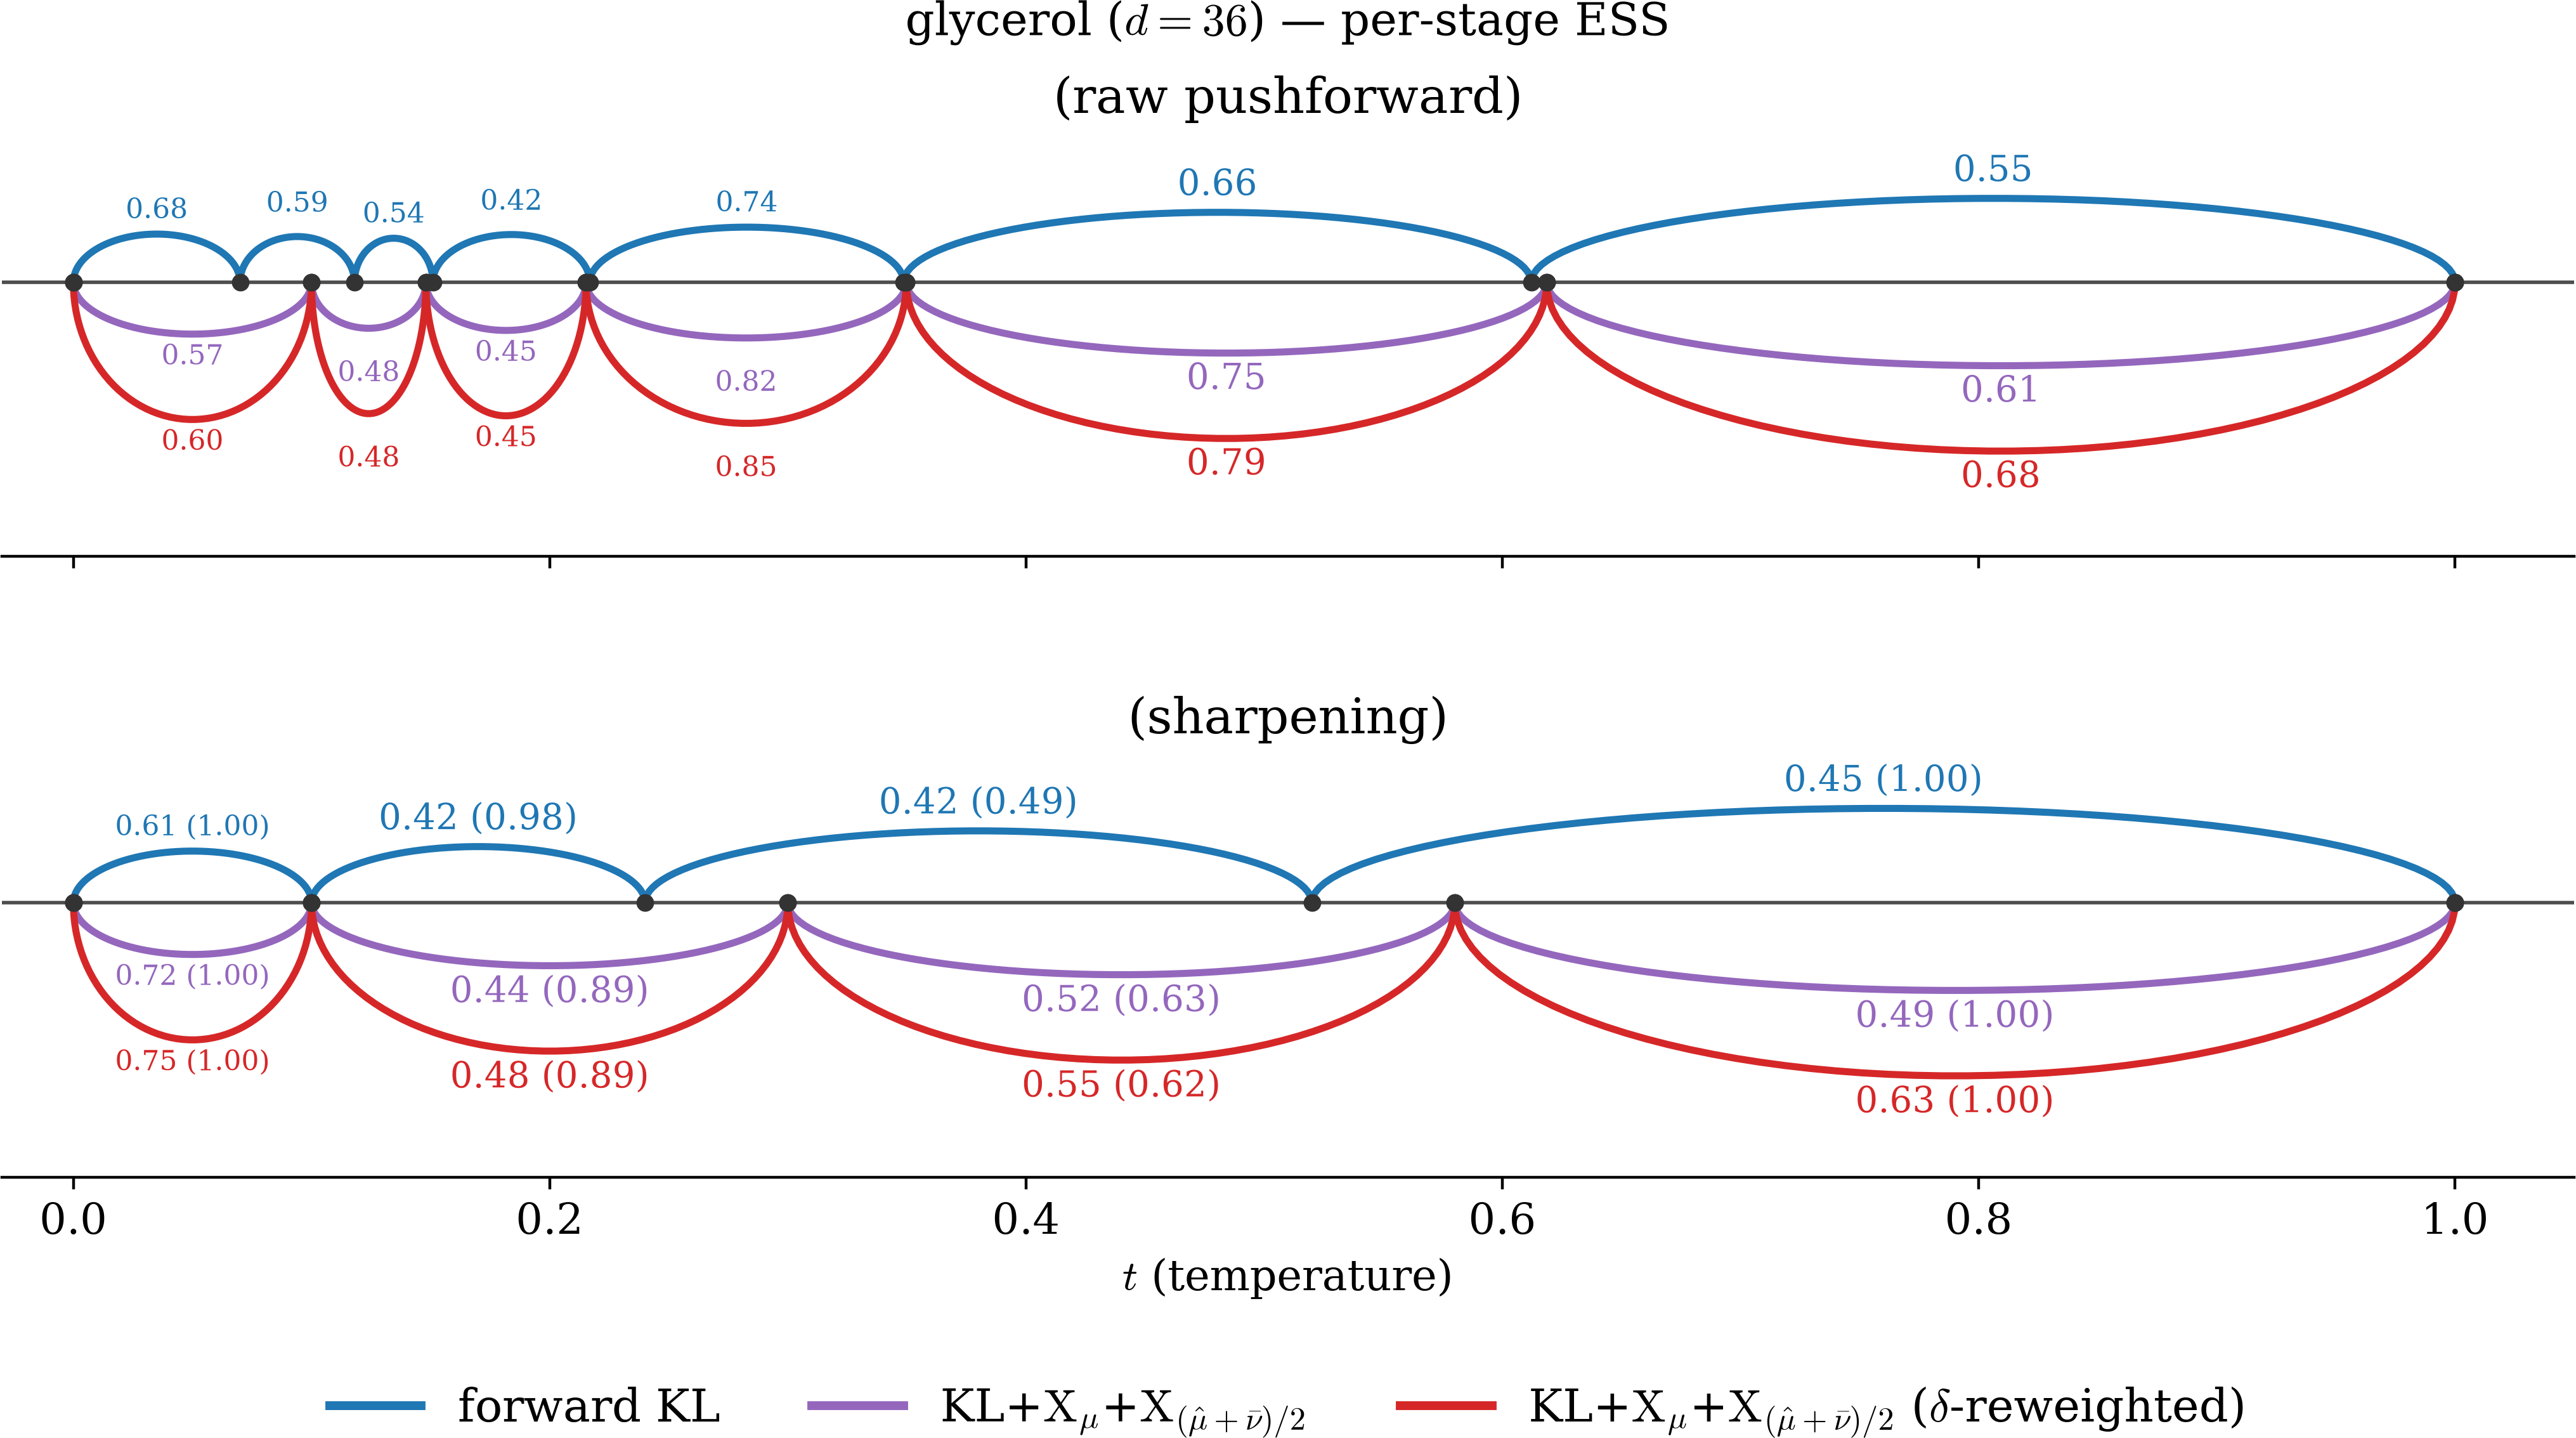
\includegraphics[width=\textwidth]{figures/Molecular_BG/glycerol_36d/ladder.png}
    \caption{Glycerol per-stage validation $\ESS$ as annealing-ladder arcs, raw (top) and sharpen (bottom).
    In each row forward KL is drawn above the axis (blue), $\KL{+}\X_\mu{+}\X_{(\hat\mu+\bar\nu)/2}$ below
    (purple), and its $\delta$-reweighted variant further below (red). Each arc is an accepted stage; the apex
    label is that stage's validation $\ESS$; a cross marks a bridge the ladder failed to reach.}
    \label{fig: glycerol-ladder}
\end{figure}

Glycerol is achiral (each torsion marginal is even, $p(\phi) = p(-\phi)$; Figure~\ref{fig: glycerol-dihedrals}), and every rotatable torsion is
three-fold: gauche$^{\pm}$ near $\pm 60^\circ$ and trans near $180^\circ$. The $\pm\phi$ symmetry pairs
gauche$^{-}\!\leftrightarrow$\,gauche$^{+}$ and leaves trans self-symmetric. The joint target over the five
rotatable torsions is therefore combinatorially multimodal (dozens of conformers), which the wide-coverage pool
must cover.


\begin{figure}[htb]
    \centering
    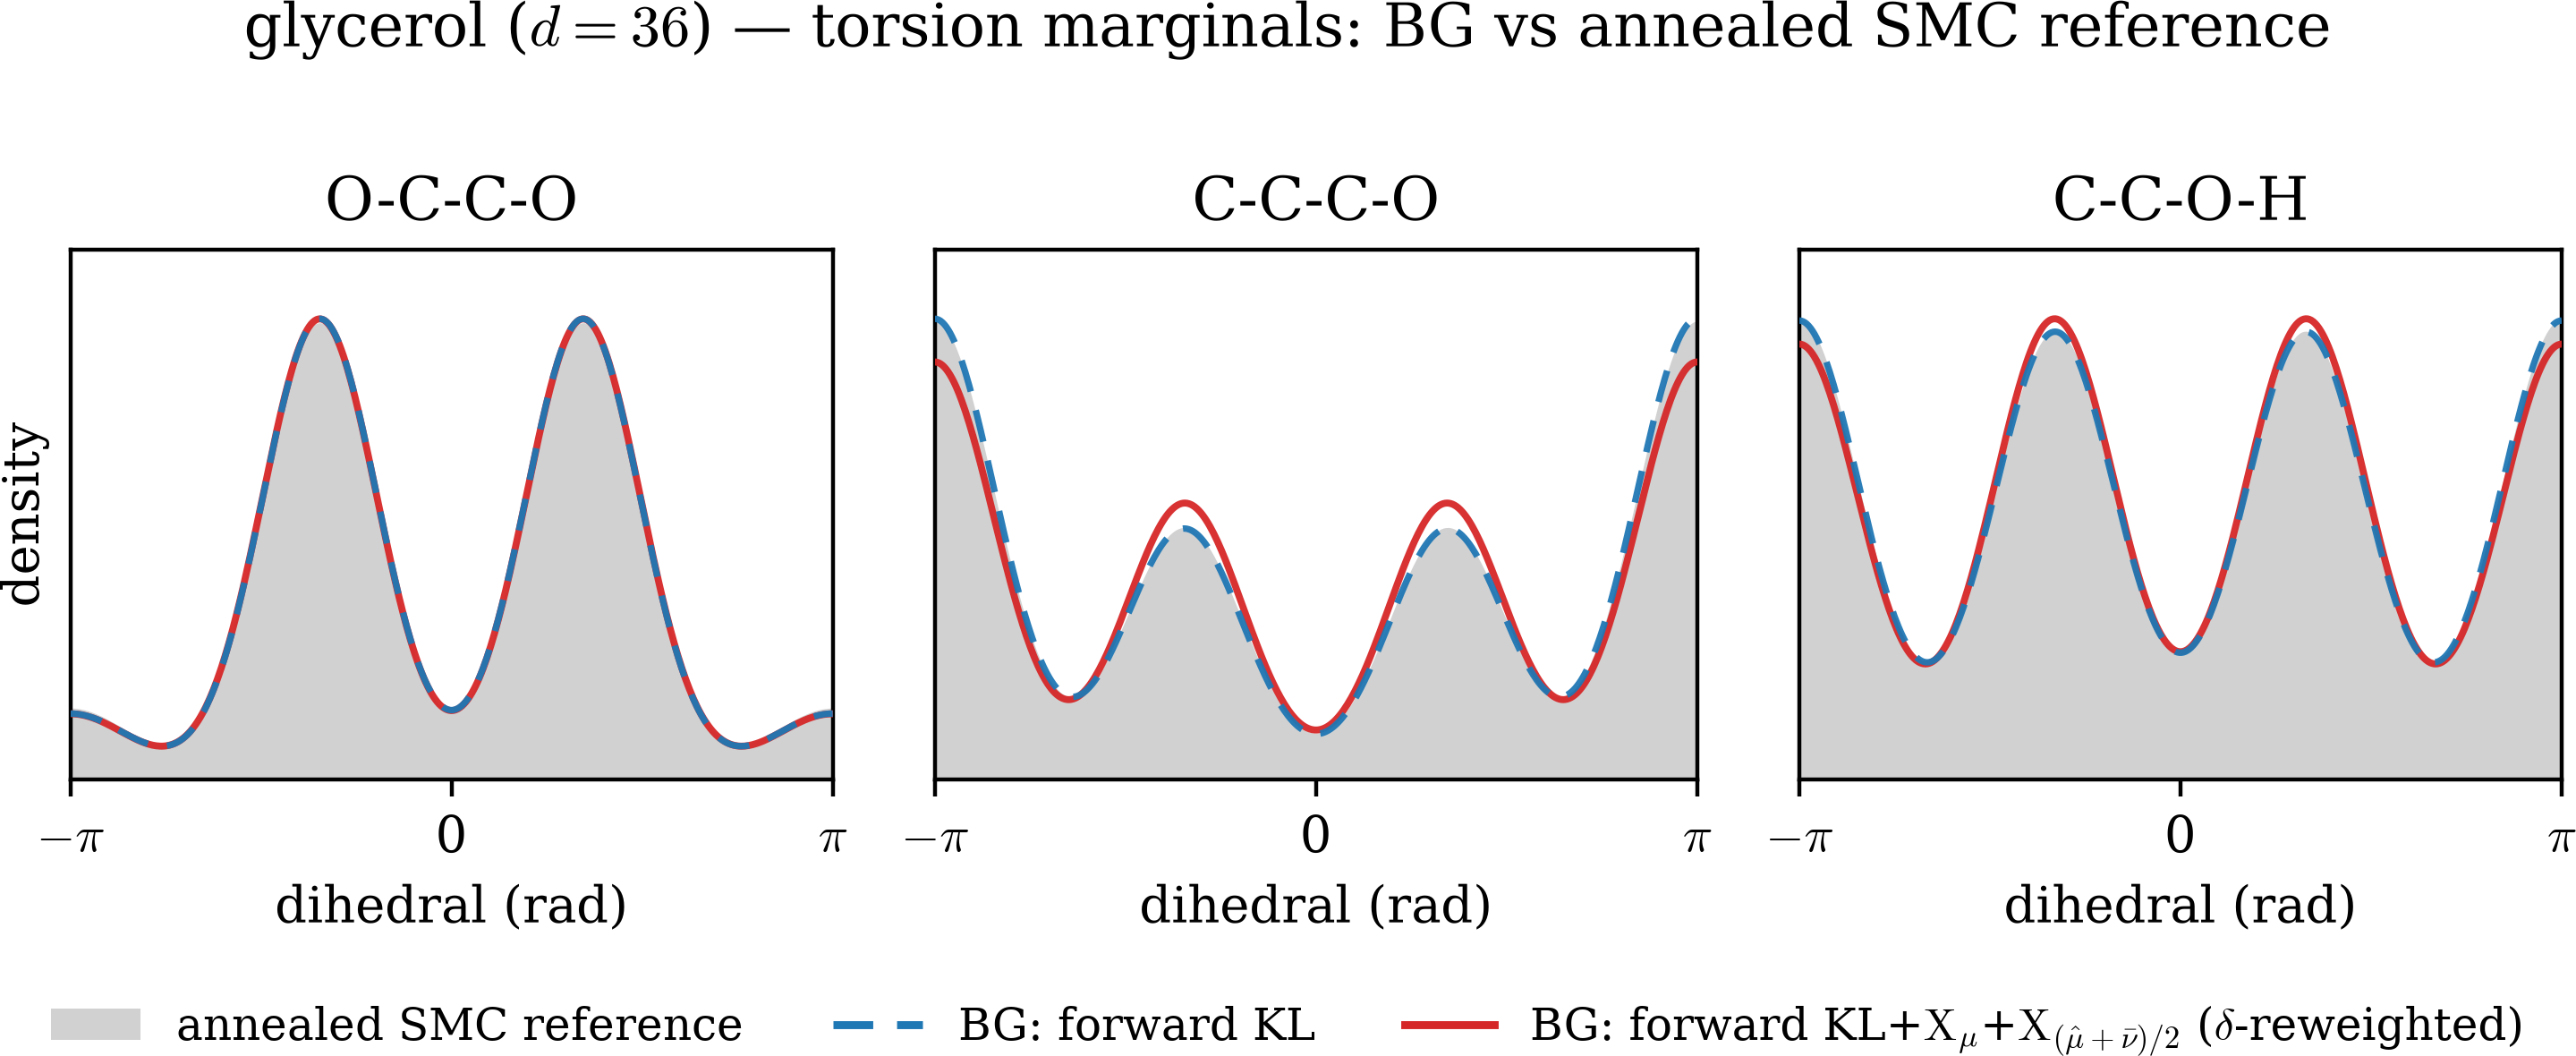
\includegraphics[width=0.8\textwidth]{figures/Molecular_BG/glycerol_36d/dihedrals.png}
    \caption{Glycerol torsion marginals of both generators against a converged annealed SMC reference
    (grey): forward KL (blue) and
    $\KL{+}\X_\mu{+}\X_{(\hat\mu+\bar\nu)/2}$, $\delta$-reweighted (red), both sharpened with the cap annealed
    to $e_{\mathrm{cap}} = 200$ kJ/mol. Both recover the multimodal gauche$^{\pm}$/trans structure of the characteristic glycerol
    torsions.}
    \label{fig: glycerol-dihedrals}
\end{figure}

\FloatBarrier
\subsubsection{Diethanolamine ($d = 48$)}
\label{sec: dea}

We test the generator on the full internal-coordinate diethanolamine target (\mbox{HN(CH$_2$CH$_2$OH)$_2$},
$d = 48$), comparing the two best losses under the same sharpening schedule (the soft cap geometrically
annealed $e_{\mathrm{cap}}\!:\!100\!\to\!200$ kJ/mol, a Monte Carlo sharpening step per stage): forward KL, and the X-regularized
$\KL{+}\X_\mu{+}\X_{(\hat\mu+\bar\nu)/2}$ with the $\delta$-reweighted quench and temper ($\delta = 0.1$).
Forward KL reaches $t = 1$ in $K = 6$ stages, the X-regularized loss in $K = 5$, a single direct
$0.65 \to 1$ step.

\begin{table}[htb]
    \centering
    \small
    \begin{tabular}{@{}lccc@{}}
        \toprule
        loss & $K$ & wall (min) & $F$ \\
        \midrule
        annealed SMC                                            & 10 & 7 & 1455.44 \\
        forward KL                                              & 6 & 896 & 92.60 \\
        $\KL{+}\X_\mu{+}\X_{(\hat\mu+\bar\nu)/2}$, $\delta$-rw. & 5 & 782 & \textbf{35.90} \\
        \bottomrule
    \end{tabular}
    \caption{Diethanolamine ($d = 48$): two trained-flow losses and an annealed SMC reference, all with
    a per-stage Monte Carlo sharpening reweight (cap $e_{\mathrm{cap}}$ geometrically annealed $100 \to 200$ kJ/mol): ladder length
    $K$, training wall-clock, and the error-propagation factor $F$ \eqref{eq: F} (smaller better; $F$ includes
    the sharpening reweight). $\delta$-rw.\ $=$
    $\delta$-reweighted quench and temper.}
    \label{tab: dea}
\end{table}

The X-regularized loss with $\delta$-reweighting reaches a lower $F$ than forward KL (Table~\ref{tab: dea}), a
${\sim}2.6\times$ reduction in importance-weight waste at identical settings (glycerol showed a comparable
${\sim}3.1\times$ gap). The advantage shows in the late, sharp stages and in the ladder
length. Forward KL's per-stage validation $\ESS$ stalls and it needs $6$ stages to reach
$t = 1$, whereas the $\KL{+}\X_\mu{+}\X_{(\hat\mu+\bar\nu)/2}$, $\delta$-reweighted run holds a higher $\ESS$
and reaches $t = 1$ in $5$ (Figure~\ref{fig: dea-ladder}). This target is singular, high-dimensional, and
combinatorially multimodal, so each run is a multi-hour computation. Closing it efficiently is the practical
contribution of the X-regularized loss.

\begin{figure}[htb]
    \centering
    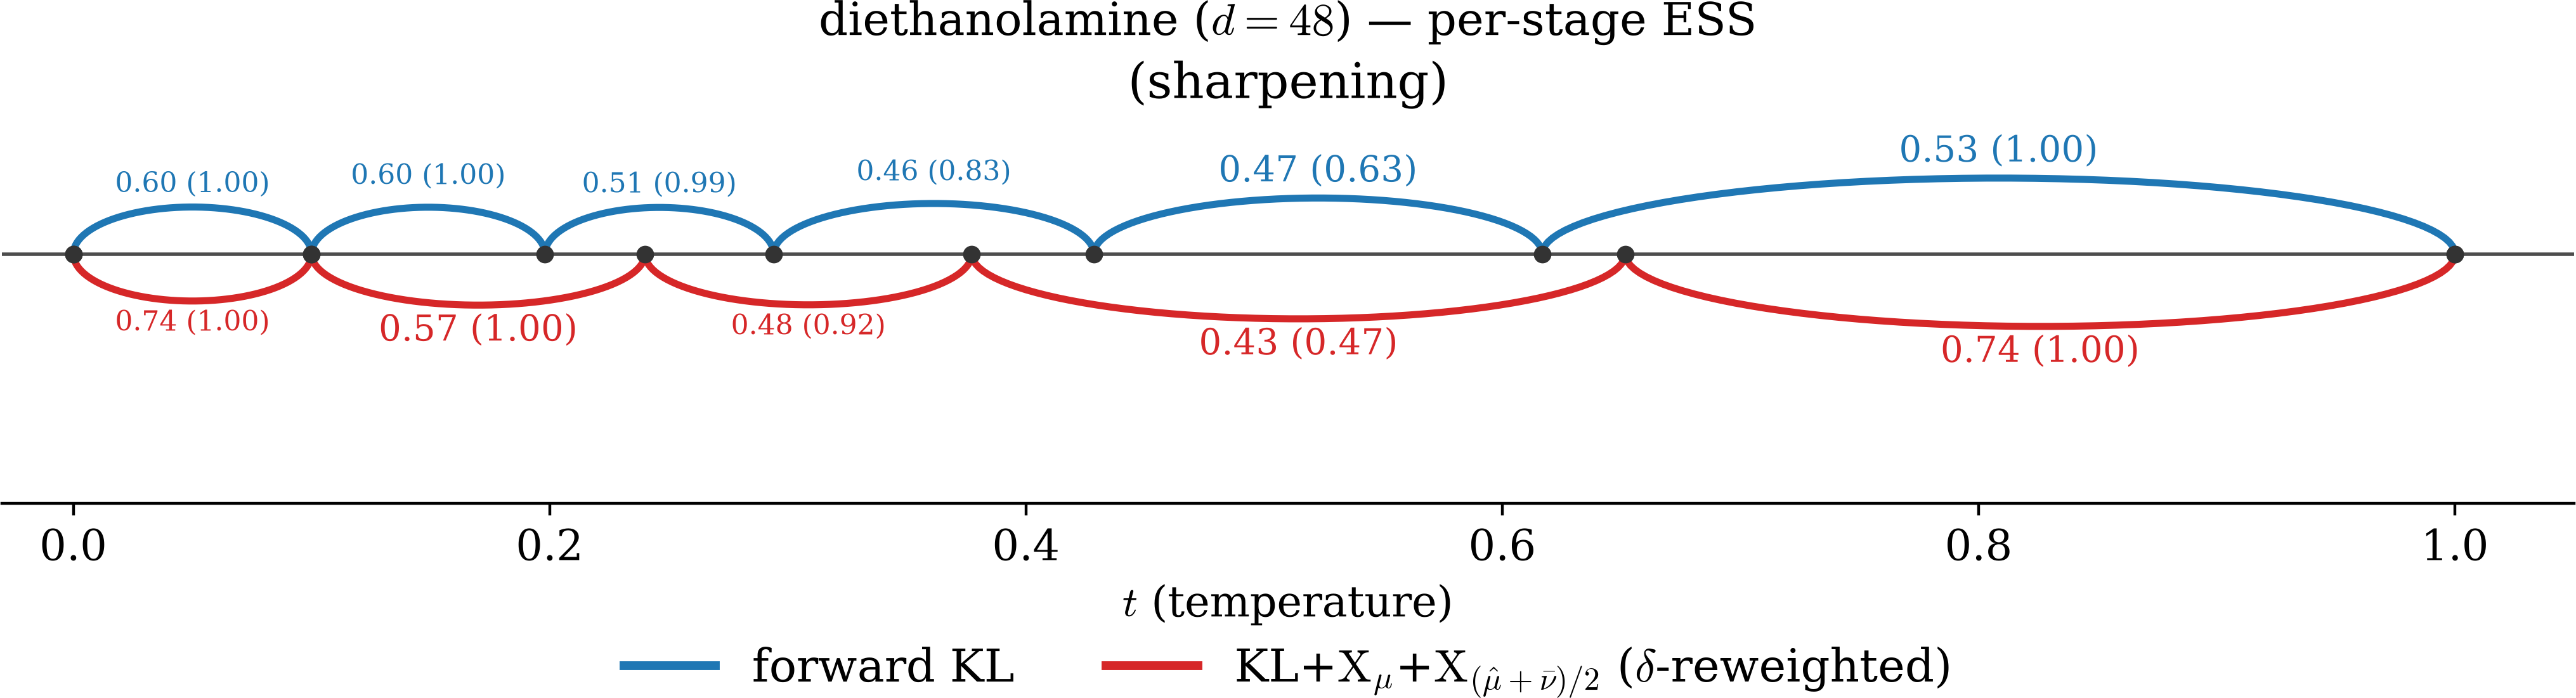
\includegraphics[width=\textwidth]{figures/Molecular_BG/diethanolamine_48d/ladder.png}
    \caption{Diethanolamine per-stage $\ESS$ as annealing-ladder arcs (sharpening schedule): forward KL above
    the axis (blue), $\KL{+}\X_\mu{+}\X_{(\hat\mu+\bar\nu)/2}$, $\delta$-reweighted, below (red). Each arc is an
    accepted stage; the apex label is that stage's validation $\ESS$, with the sharpening $\ESS$ in
    parentheses.}
    \label{fig: dea-ladder}
\end{figure}

Diethanolamine has a plane of symmetry (each torsion marginal is even, $p(\phi) = p(-\phi)$). Its rotatable
backbone torsions, O-C-C-N and C-C-N-C along the ethanolamine arms plus the hydroxyl rotations,
are each multi-well (gauche$^{\pm}$/trans), so the joint target is combinatorially multimodal, which the
wide-coverage pool must cover.


\begin{figure}[htb]
    \centering
    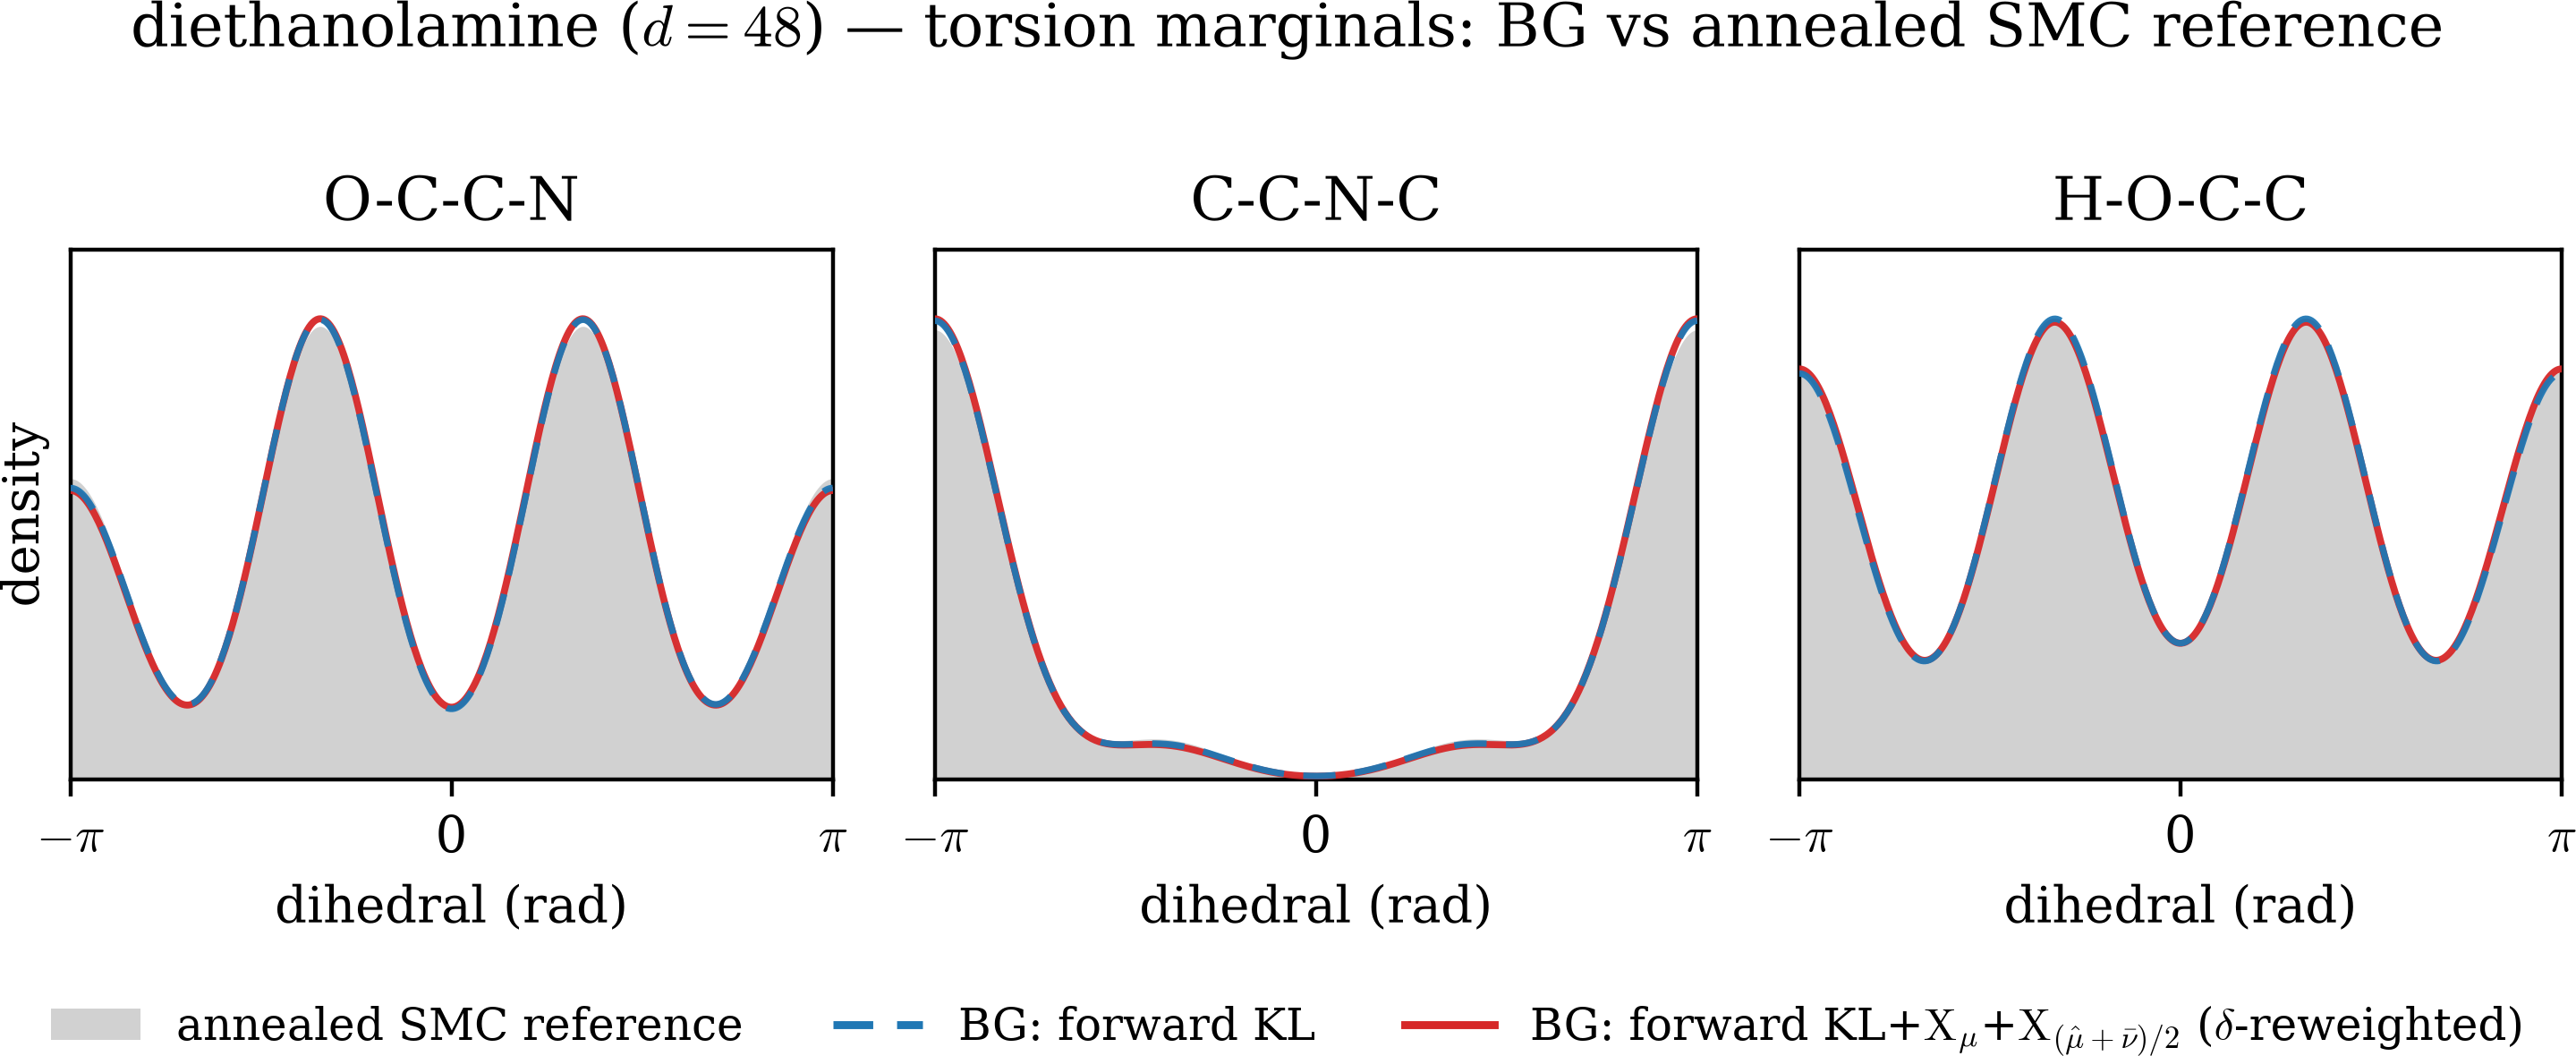
\includegraphics[width=0.8\textwidth]{figures/Molecular_BG/diethanolamine_48d/dihedrals.png}
    \caption{Diethanolamine torsion marginals of both generators against a converged annealed SMC
    reference (grey): forward KL (blue) and
    $\KL{+}\X_\mu{+}\X_{(\hat\mu+\bar\nu)/2}$, $\delta$-reweighted (red), both sharpened with the cap annealed
    to $e_{\mathrm{cap}} = 200$ kJ/mol. Both recover the multimodal backbone torsions and track the annealed SMC reference.}
    \label{fig: dea-dihedrals}
\end{figure}

Against the annealed SMC reference (Figure~\ref{fig: dea-dihedrals}) the two losses are visually indistinguishable: both
recover the multimodal backbone torsions, and neither is closer to the reference. The separation is in
efficiency, not in the sampled marginals. $\KL{+}\X_\mu{+}\X_{(\hat\mu+\bar\nu)/2}$ reaches $t = 1$ in fewer
stages, with a higher final-step $\ESS$, a $\sim 2.6\times$ smaller
error-propagation factor, and fewer rejected stage attempts in the early ladder. Switching the trained flow off entirely (the
identity map at every stage, i.e.\ plain adaptive annealed SMC over the same ladder) gives a far larger $F$. The trained
X-regularized flow therefore cuts the propagation factor by ${\sim}40\times$ and halves the ladder length
($5$ vs $10$). On this singular target the transport map adds even more over annealing alone than on glycerol,
a justification for training a flow.

\FloatBarrier
\subsubsection{Alanine dipeptide ($d = 60$)}
\label{sec: adp}

We push the generator to alanine dipeptide (Ac-Ala-NHMe), the canonical Boltzmann generator benchmark,
in full internal coordinates ($d = 60$). The step up from glycerol and diethanolamine is the
target's character. Those are dominated by smooth rotatable-bond multimodality. Alanine dipeptide folds the backbone
tightly enough that the Lennard-Jones clash core, not the torsion profile, sets the hardest part of the
anneal. We report the X-regularized loss only ($\KL{+}\X_\mu{+}\X_{(\hat\mu+\bar\nu)/2}$,
$\delta$-reweighted, $\delta = 0.1$), with a per-stage Monte Carlo sharpening in which \emph{both} the cap
$e_{\mathrm{cap}}\!:\!100\!\to\!200$ kJ/mol and the clash floor $r_{\mathrm{floor}}\!:\!0.2\!\to\!0.1$ nm are annealed arithmetically, unlike the geometric
$e_{\mathrm{cap}}$ schedule of glycerol and diethanolamine. Alanine dipeptide is also the only target that anneals $r_{\mathrm{floor}}$, which glycerol and diethanolamine hold fixed at $0.1$ nm. The run reaches $t = 1$ in $K = 11$ stages,
every stage holding a high validation and sharpening $\ESS$
(Table~\ref{tab: adp}, Figure~\ref{fig: adp-ess}). The bare composed flow's end-to-end $\ESS$ against the sharp
target, from a single importance reweight of source samples pushed through the fully composed $K$-stage map and
scored against $U_{1,1}$, is only ${\sim}5\times10^{-6}$, so the per-stage sharpening, not a raw pushforward,
is the deliverable.

\begin{table}[htb]
    \centering
    \small
    \begin{tabular}{@{}lccc@{}}
        \toprule
        loss & $K$ & wall (min) & $F^{*}$ \\
        \midrule
        annealed SMC                                           & 12 & 23  & 129.70$^{*}$ \\
        $\KL{+}\X_\mu{+}\X_{(\hat\mu+\bar\nu)/2}$, $\delta$-rw. & 11 & ${\sim}1000$ & \textbf{67.95}$^{*}$ \\
        \bottomrule
    \end{tabular}
    \caption{Alanine dipeptide ($d = 60$), the X-regularized loss with a per-stage Monte Carlo sharpening
    reweight (the cap $e_{\mathrm{cap}}$ and floor $r_{\mathrm{floor}}$ annealed arithmetically): ladder length $K$,
    wall-clock, and the error-propagation factor $F^{*}$ \eqref{eq: Fstar}, starred throughout because every
    entry uses the smooth validation $\ESS$ (smaller better; $F^{*}$ includes the sharpening reweight). The
    first row is an annealed SMC reference, the identity map over the same ladder.
    $\delta$-rw.\ $=$ $\delta$-reweighted quench and temper.}
    \label{tab: adp}
\end{table}

Compared with the lighter targets, alanine dipeptide's larger $F^{*}$ is the price of its singular nonbonded core, not of its multimodality. Three
alanine-dipeptide-only factors make this $F^{*}$ read smaller than a strict like-for-like extension of that trend:
the per-stage $\ESS$ is the smooth estimator $\ESS^{\mathrm{val}*}_k$ \eqref{eq: smooth-ess} rather than the raw weighted
$\ESS$; $r_{\mathrm{floor}}$ is annealed alongside the cap; and the ladder is longer ($K = 11$
versus $4$ and $5$), its smaller per-step jumps keeping each per-stage $\ESS$ high. All three raise the
per-stage $\ESS$ entering $F^{*}$, and none applied to the lighter targets.

\begin{figure}[htb]
    \centering
    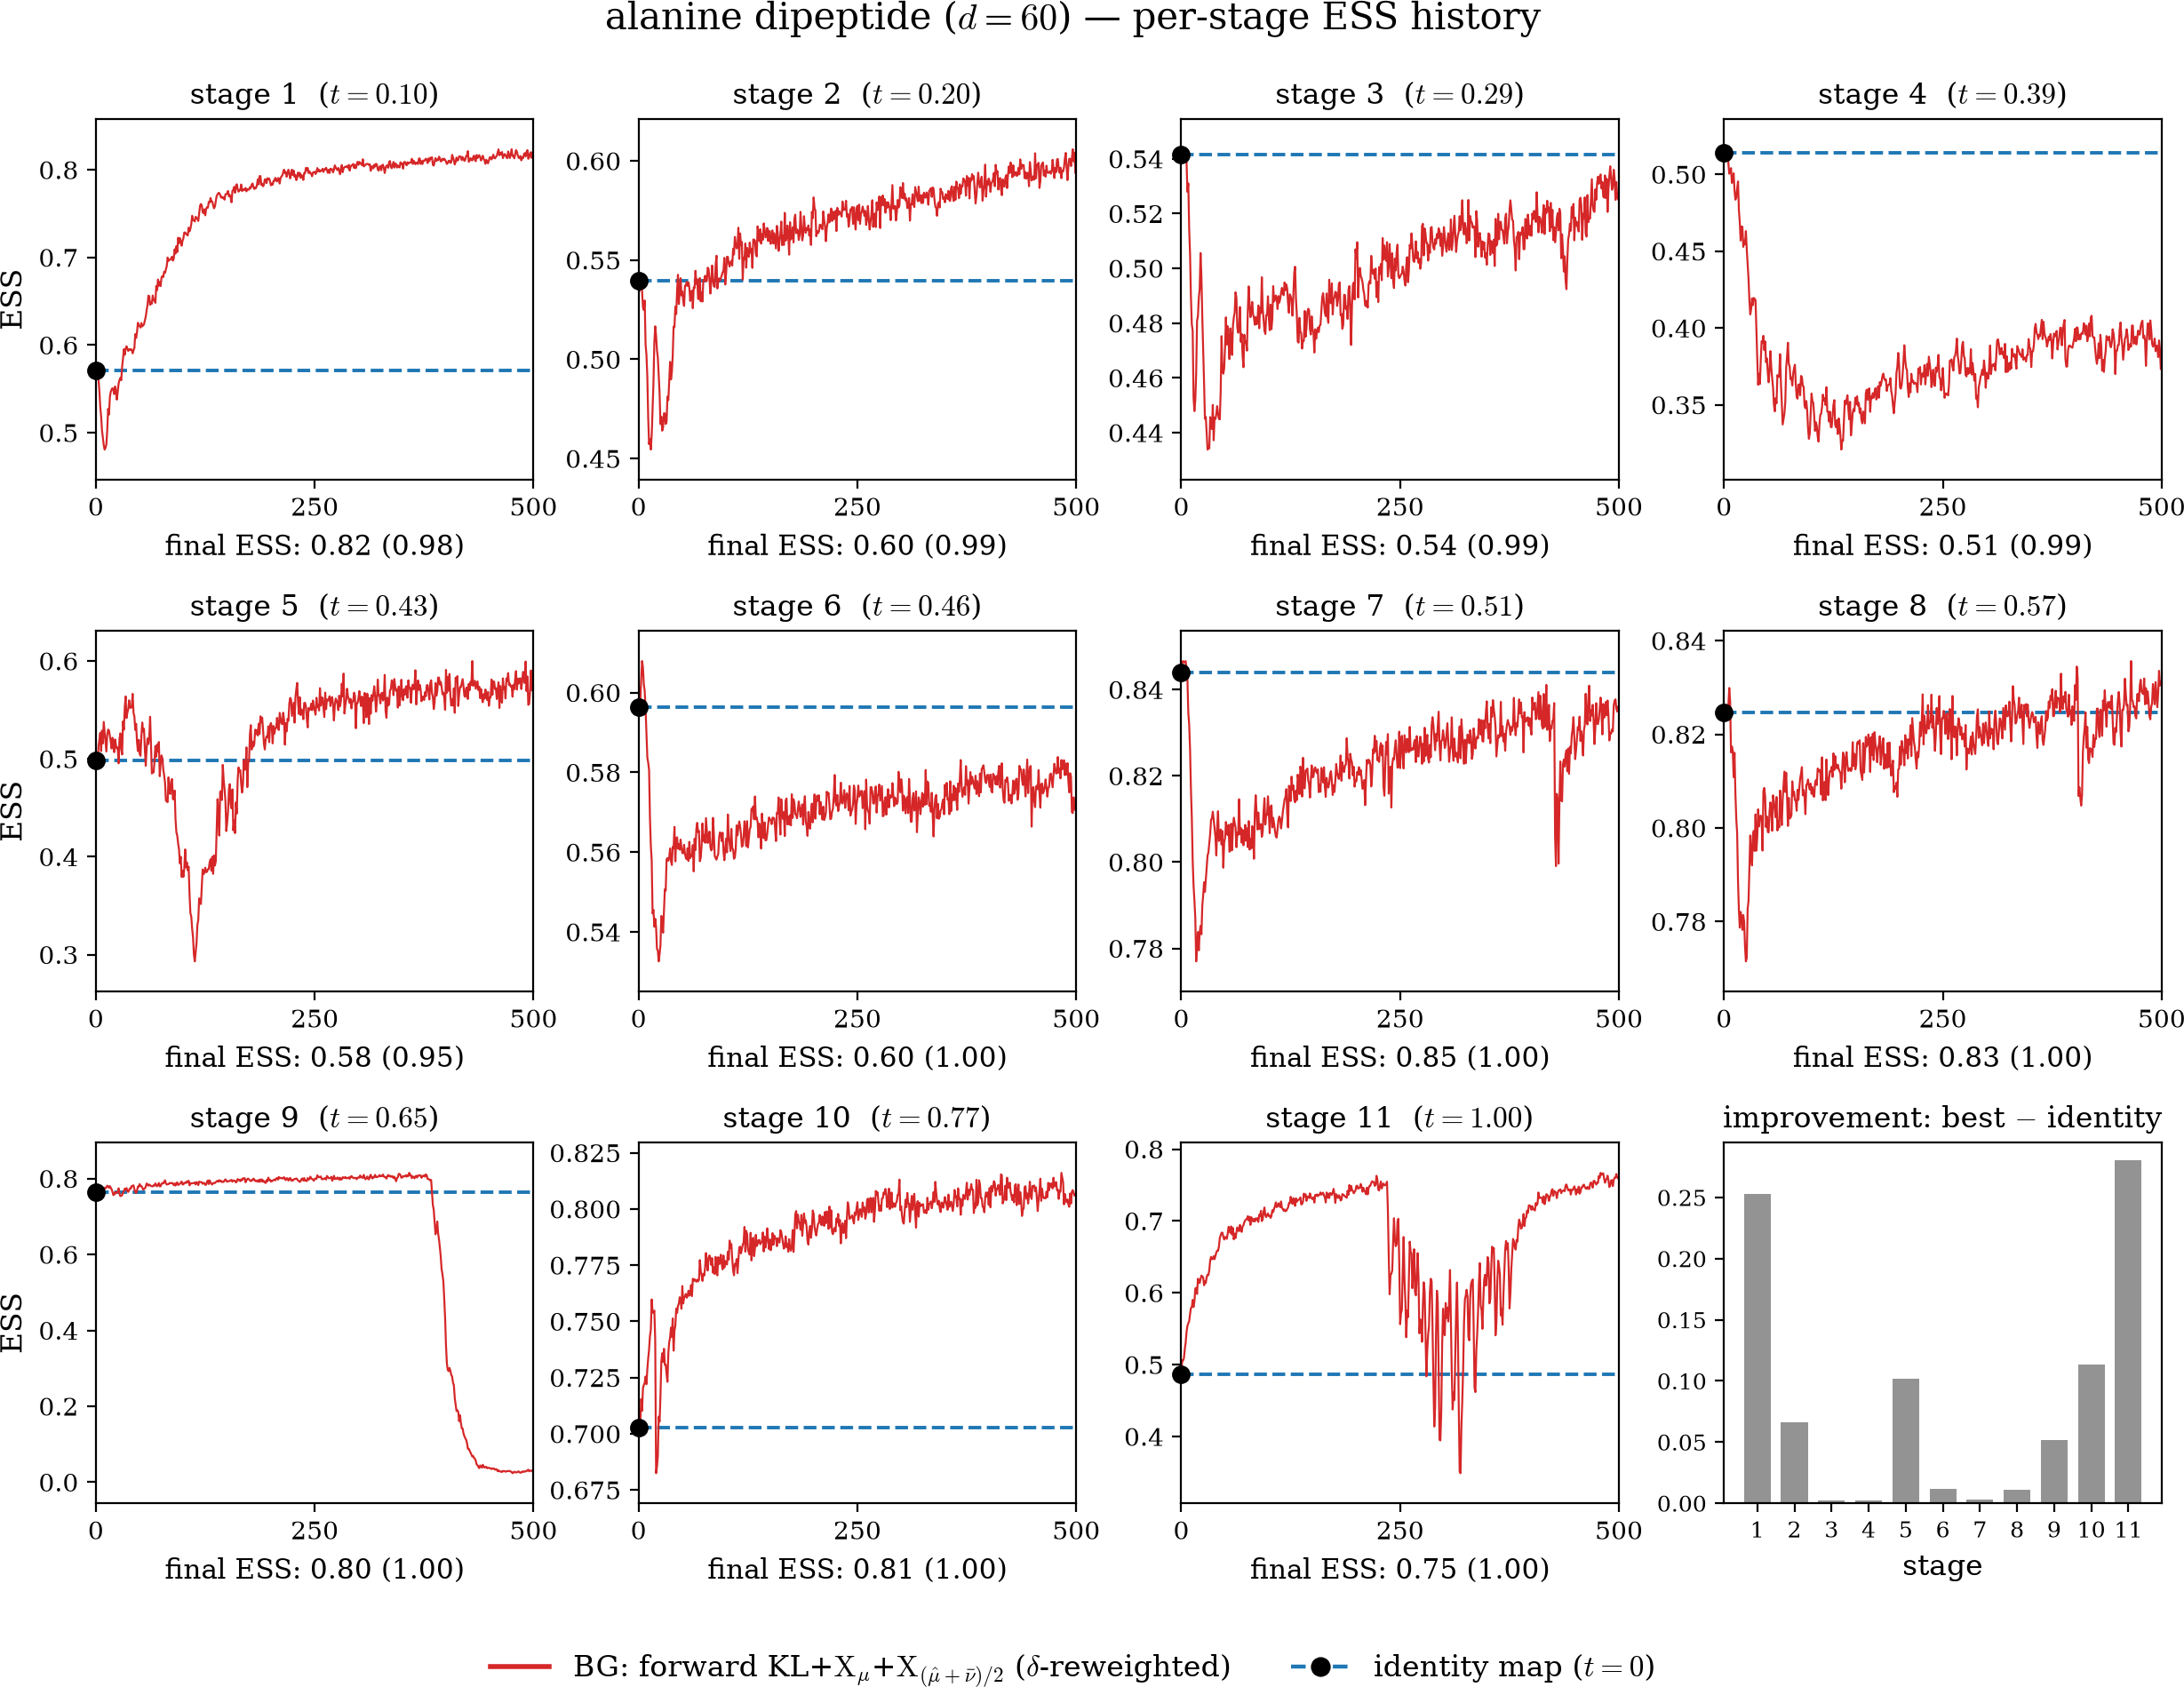
\includegraphics[width=\textwidth]{figures/Molecular_BG/adp_60d/ess_history.png}
    \caption{Alanine dipeptide per-stage $\ESS$ history: each panel is the per-step effective sample size
    during that stage's X-regularized $\delta$-reweighted flow training (red), against the identity-map
    baseline at $t = 0$ (blue dashed). Below each panel is that stage's accepted validation $\ESS$ with the
    sharpening $\ESS$ in parentheses. The dip across $t \approx 0.29$--$0.43$ is the clash bottleneck, with
    $\ESS$ recovering to $\approx 0.8$ once the cap is sharp enough to separate the basins.}
    \label{fig: adp-ess}
\end{figure}

The instability is localized to a clash bottleneck near $t \approx 0.3$--$0.43$. The stages spanning
$t \approx 0.29$--$0.43$ (soft cap $e_{\mathrm{cap}} \approx 129$--$143$ kJ/mol) are where the nonbonded core first bites: the run
minimum validation $\ESS$ sits here, and these are the only stages that shrink
the step or retry heavily. Below
$t \approx 0.3$ the torsions dominate and the flow trains in a single attempt. Above $t \approx 0.5$ the
cap is sharp enough that the basins separate cleanly and $\ESS$ recovers to ${\approx}0.8$. The binding
constraint for alanine dipeptide is the clash singularity, not the multimodality. This is the qualitative difference from the
$d \Le 48$ molecules, and the reason the three devices of Section~\ref{sec: mol-engineering} (particle drop,
best $\ESS$ gate snapshots, $r$-floor anneal), inert on glycerol and diethanolamine, were necessary here.

The per-stage $\ESS$ history (Figure~\ref{fig: adp-ess}) exposes two coupled instabilities that the best $\ESS$
gate works around but does not cure. First, the within-stage $\ESS$ is \emph{non-monotone and unstable}: it
can rise, plateau, then drop abruptly (the collapse late in the $t = 0.65$ stage and the volatility at
$t = 1$ are the clearest cases), so the last training step is often far below the best. Second, near the clash bottleneck ($t \approx 0.3$--$0.5$) several flows \emph{degenerate
toward the identity map}: the best achievable $\ESS$ barely exceeds the $t = 0$ identity baseline, i.e.\ training fails to improve on
doing nothing. Both follow from the \emph{singularity of the potential}: the Lennard-Jones
$r \to 0$ divergence leaves the soft-capped target ill-conditioned where the nonbonded core first
bites, so the gradient signal that would pull the flow off identity is weakest there. We report this as a
known limitation; remedies (stronger or adaptive regularization annealing, parameterizations tailored
to the repulsive wall) are left to future work.

\begin{figure}[htb]
    \centering
    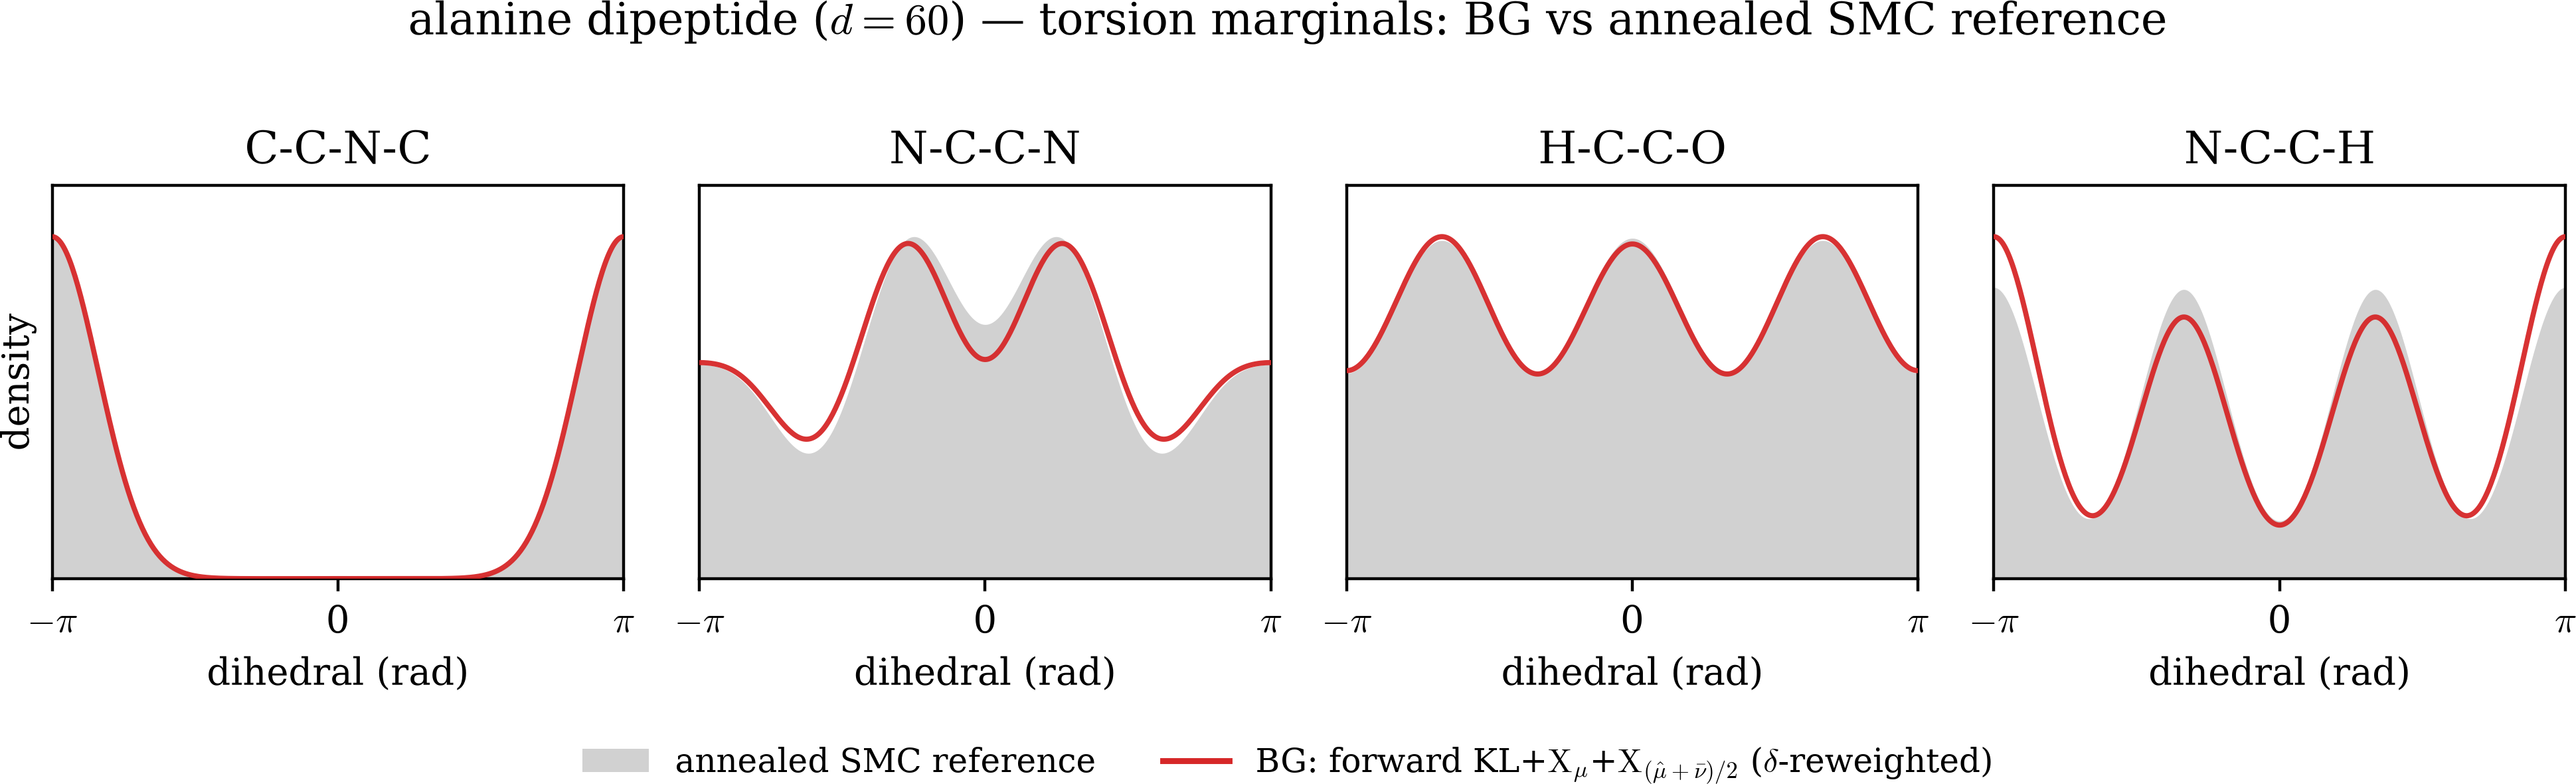
\includegraphics[width=\textwidth]{figures/Molecular_BG/adp_60d/dihedrals.png}
    \caption{Alanine dipeptide torsion marginals of the BG deliverable (red) against a converged
    annealed SMC reference (grey). The four most multimodal proper
    torsions are shown; the densities are $\pm\phi$-symmetrised, the achiral target having $p(\phi) = p(-\phi)$.
    The BG recovers the multimodal backbone torsions and tracks the reference; the peptide-bond torsion $\omega$ (C-C-N-C) is
    trans-dominant in the generator, the one torsion whose high rotation barrier also makes the uniform-init annealed SMC
    reference slow to converge.}
    \label{fig: adp-dihedrals}
\end{figure}

Alanine dipeptide's backbone $\phi,\psi$ are multi-basin (Figure~\ref{fig: adp-dihedrals}). A second, alanine-dipeptide-specific feature
is chirality: the classical force field is mirror-symmetric (every term in \eqref{eq: amber} is invariant
under reflection), so the L- and D-forms are isoenergetic, and the internal-coordinate flow, carrying no
chirality constraint, emits \emph{both} where a physical trajectory would stay in one. In the Ramachandran (Figure~\ref{fig: adp-rama}) this appears as the $(\phi,\psi)\!\to\!(-\phi,-\psi)$ point symmetry, the D-basins mirroring the L-basins, each populated.

\begin{figure}[htb]
    \centering
    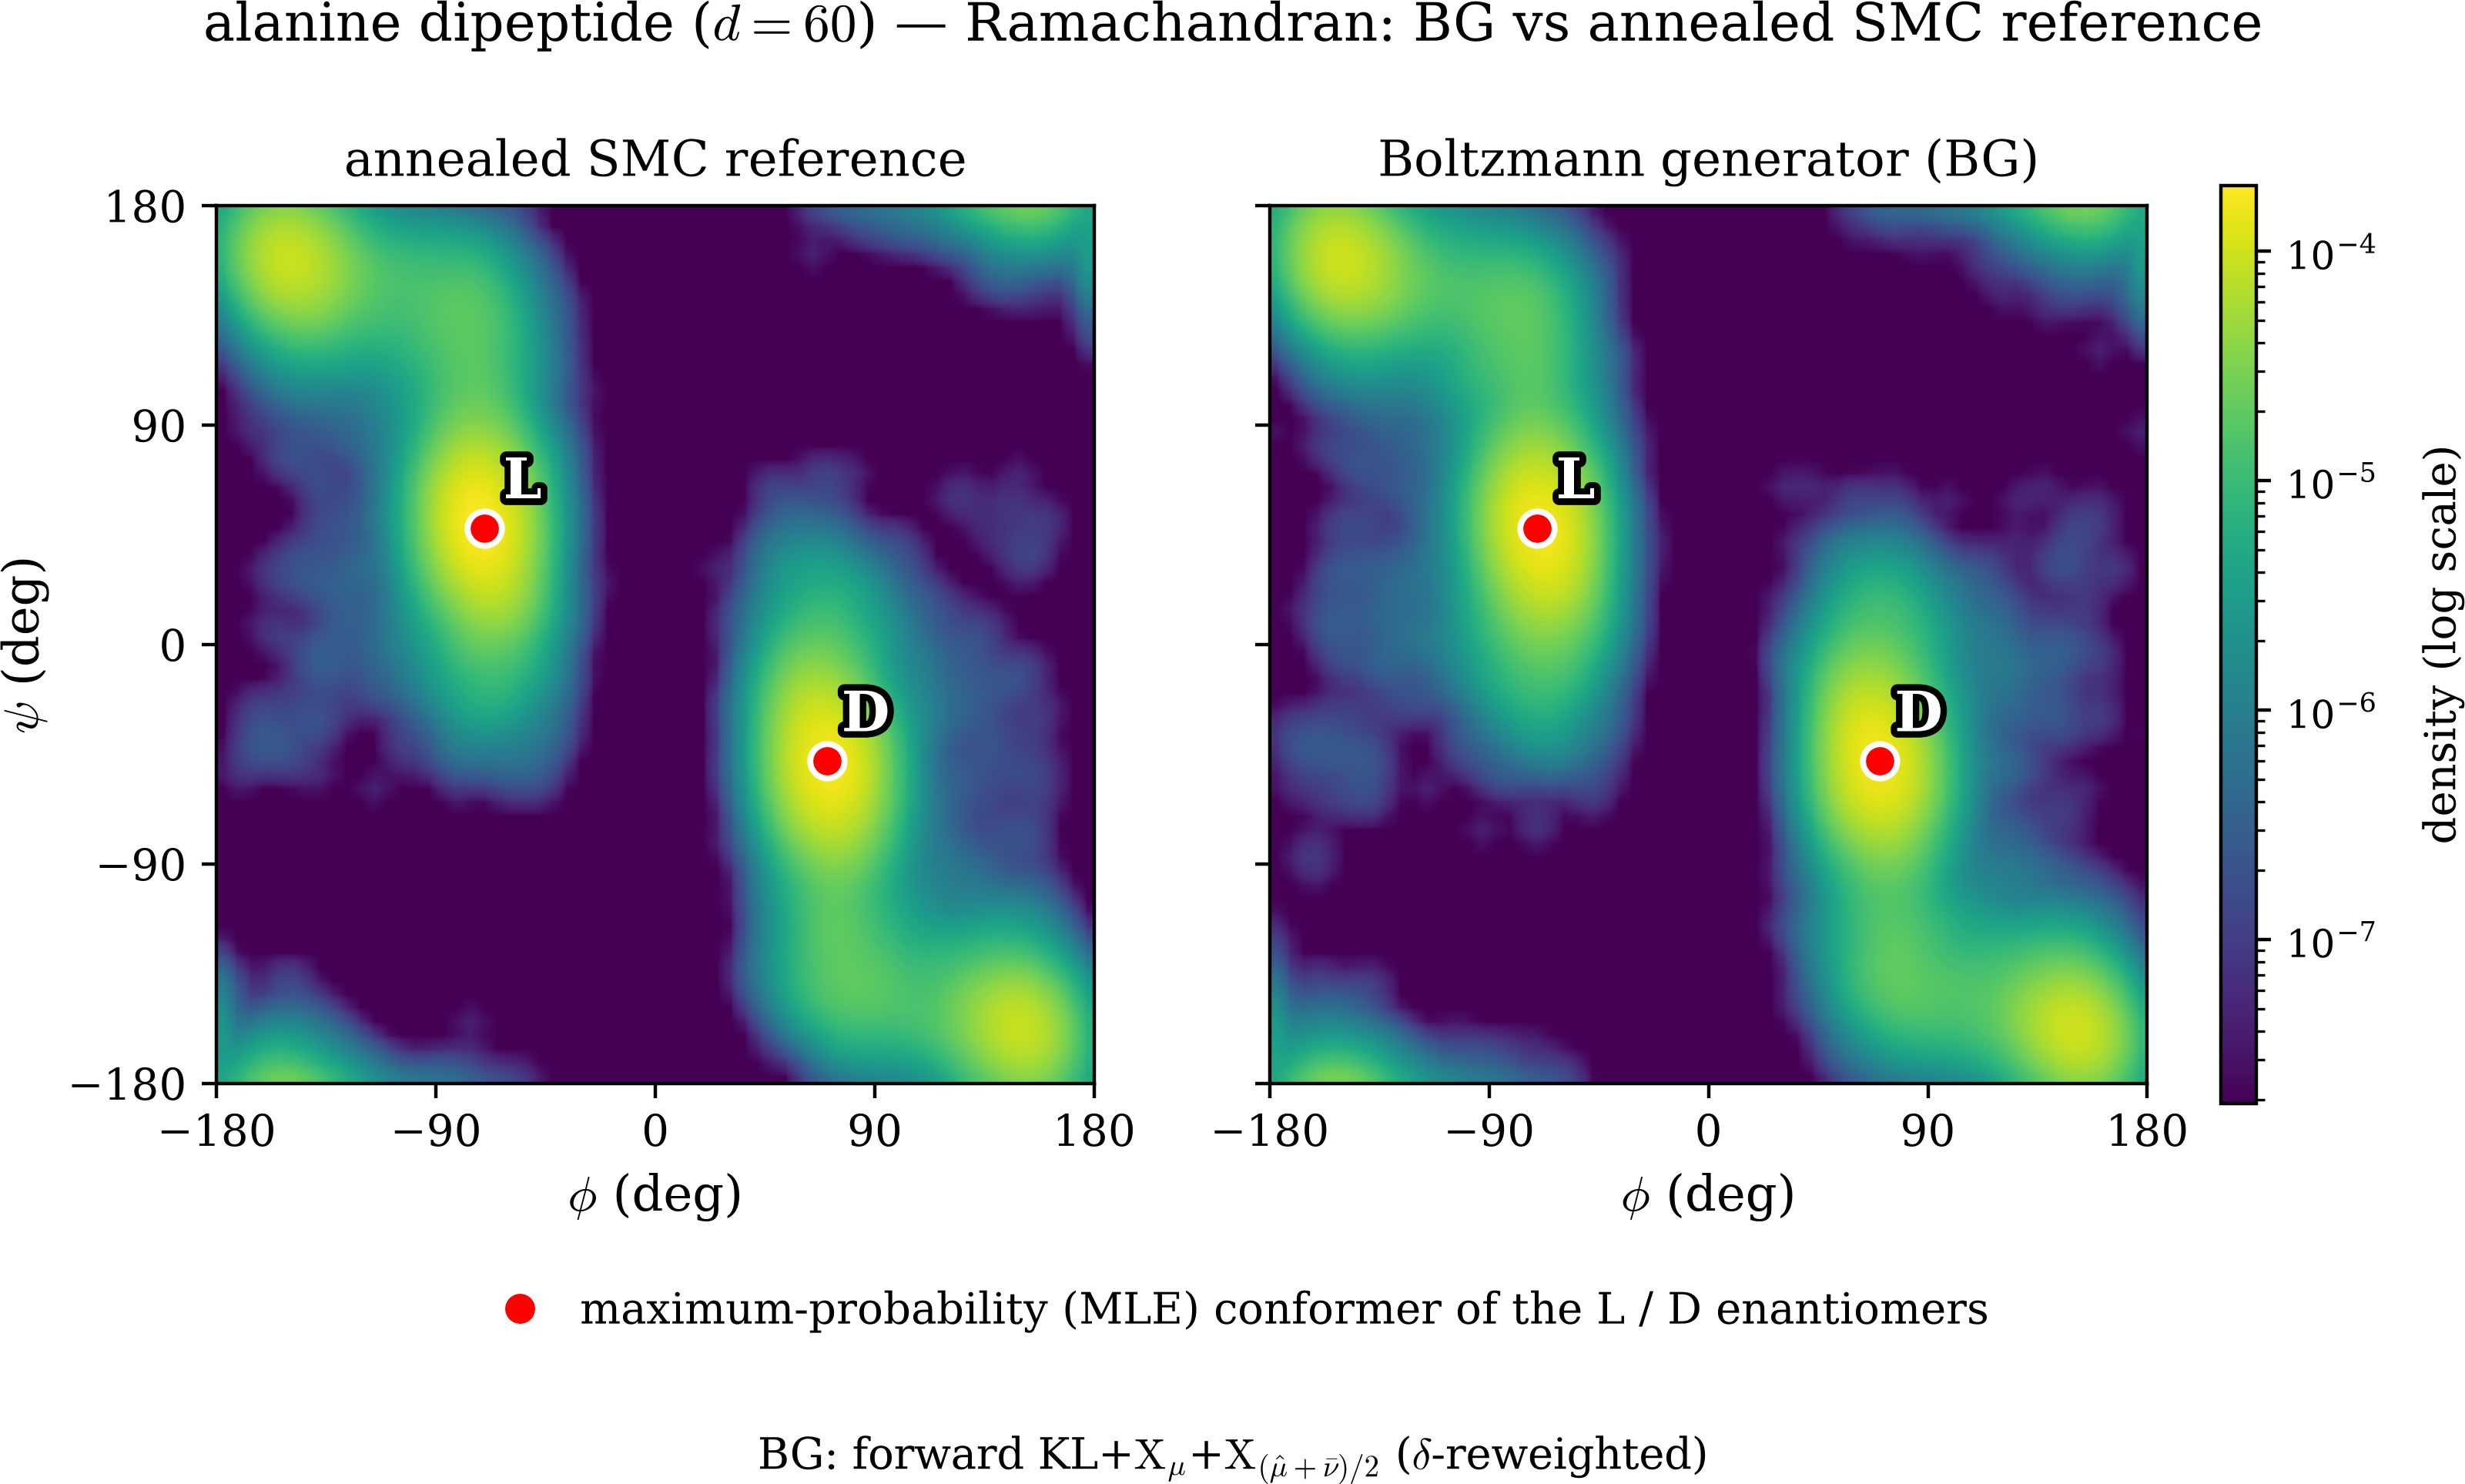
\includegraphics[width=0.92\linewidth]{figures/Molecular_BG/adp_60d/ramachandran.png}
    \caption{Alanine dipeptide Ramachandran ($\phi,\psi$), shared log-density scale: the BG deliverable
    (right) against the annealed SMC reference (left). Red dots mark the maximum-probability conformer of
    each enantiomer (L at $\phi<0,\psi>0$; D at $\phi>0,\psi<0$). Both panels populate the same backbone basins
    with the $(\phi,\psi)\!\to\!(-\phi,-\psi)$ point symmetry: the achiral vacuum force field makes the L- and
    D-enantiomers isoenergetic, and the generator, carrying no chirality constraint, samples both.}
    \label{fig: adp-rama}
\end{figure}

The X-regularized BG closes the full internal-coordinate alanine dipeptide target to $t = 1$ in $11$ stages,
recovering the multimodal backbone torsions against a converged annealed SMC reference and emitting both
chiral forms of the mirror-symmetric target. The lesson from the lighter $d \Le 48$ molecules is
inverted: alanine dipeptide's difficulty is not its combinatorial torsion multimodality but its nonbonded clash core,
concentrated in the $t \approx 0.3$--$0.43$ stages, which the particle drop,
best $\ESS$ gate snapshots, and $r$-floor anneal together make tractable. Across all three molecules the
pattern is consistent: the sharpening split makes the singular target trainable at all, and the
X-regularized flow then earns a ${\sim}30$--$40\times$ reduction in importance-weight waste where the landscape is
multimodal but clash-mild, narrowing to ${\sim}2\times$ where the singularity dominates.

\subsection{Limitations}
\label{sec: mol-limitations}

Four simplifications bound the molecular experiments, each a direction for future work. First, the
targets are evaluated in vacuum: $U_{\mathrm{FF}}$ is the isolated-molecule Amber potential \eqref{eq: amber} with no solvent
and no nonbonded cutoff. Solvation only reshapes $U_{\mathrm{FF}}$, not the sampler, and the vacuum targets already
display the well-separated potential wells the generator must discover and resolve; implicit or explicit
solvent and larger peptides are left untreated. Second, the internal-coordinate generator carries no chirality
constraint, so for the achiral Amber force field it samples both the L- and D-enantiomers
(Section~\ref{sec: adp}), whereas a physical trajectory stays in one; isolating a single enantiomer by a filter
or restraint is left to future work. Third, we do not benchmark against FAB
\citep{midgley2022flow}: its large per-step batches and replay buffer make a like-for-like comparison under the
same compute budget as these forward KL-type losses prohibitive, so the natural same-cost baselines here are
the bare forward KL and the identity-flow annealed SMC. Fourth, on the alanine dipeptide clash core the
per-stage flow training is unstable and can degenerate toward the identity map
(Section~\ref{sec: adp}); the best $\ESS$ gate works around this but does not cure it, and a regularization or
parameterization that conditions the repulsive wall remains open.



% ===================== Section 7: Conclusions + Acknowledgement (verbatim) =====================
\section{Conclusions}
\label{sec: conclusions}

Forward KL training of a normalizing flow Boltzmann generator usually trains well. But it can miss modes and report a fake effective sample size. Noisy or biased annealed samples limit its accuracy. A smaller leakage failure rides alongside, where the target vanishes. We close these gaps by regularizing the forward KL with a term that reuses the flow's own log-ratio.

\begin{itemize}
\item We propose the log-ratio variation, a family of X functionals. They augment the forward KL by penalizing the pairwise variation of $\log(\mu/\nu)$ under a non-negative weight. One forward pass of the flow computes them. The shape term costs little beyond a plain forward KL step; the mixture adds one sampling batch.
\item One regularizer takes three roles through its weight. $\X_\mu$ controls the shape of the log-ratio and stabilizes training. $\X_{\hat\mu}$ drives mode discovery, drawing the flow toward a wide-coverage measure that quench and temper prepares before training. $\X_{\bar\nu}$ suppresses leakage.
\item The balanced loss $\KL{+}\X_\mu{+}\X_{(\hat\mu+\bar\nu)/2}$ combines the three roles in one objective. It folds mode discovery and leakage suppression into a single pairwise integral. It serves as a default and needs little tuning. A Fisher--Rao analysis shows the forward KL still decays along the $\X_\mu$-regularized flow. Under a bound on the regularization strength, the $\X_\mu$ term can lower the accuracy floor that biased AIS samples leave behind. The forward KL is sensitive to these samples early in training, so the X-regularized losses help most when the training batch is small. The loss applies across smooth benchmarks, a high-dimensional multi-well, and lattice field theories, where it tends to discover modes and sharpen accuracy.
\item We build an adaptive-temperature Boltzmann generator on the loss. It grows its ladder from the SMC effective sample size. On molecular potentials, a sharpening reweight pulls each stage toward the physical potential. In our experiments it tends to improve per-stage quality and reduce importance-weight waste over annealing alone. Gains are smaller where a singular clash core, not multimodality, is the difficulty.
\end{itemize}

Several directions invite further study. First, a comparison with FAB \citep{midgley2022flow}, and a possible combination with it, would weigh our quench against its replay buffer; the same comparison extends to other AIS-based flow samplers. Second, the training instability at the singular clash core calls for a remedy that conditions the repulsive wall, since the present best $\ESS$ gate works around the instability rather than curing it. Third, larger and solvated systems are a natural target, where the potential reshapes but the sampler need not change. Finally, a JAX implementation in place of the present PyTorch one would speed up training and inference.


\section*{Acknowledgement}

The normalizing flows are built on the Python packages \texttt{zflows} and \texttt{zflows\_md}, written by the author Xuda Ye and installable through Anaconda. The source code reproducing all numerical experiments is openly available. Both are listed below:
\begin{tcolorbox}[colback=gray!12,boxrule=0pt,arc=2pt,left=6pt,right=6pt,top=4pt,bottom=4pt]
\texttt{conda install xudaye::zflows xudaye::zflows\_md}\\[3pt]
\url{https://github.com/xuda-ye-math/X-regularization}
\end{tcolorbox}
\noindent
Numerical tests run on an NVIDIA RTX 5070\,Ti GPU with $16$\,GB of VRAM.

\clearpage
\appendix

\section{Fisher--Rao gradient flow with log-ratio variation}
\label{sec: appendix-FR}

Section~\ref{sec: FR} states the main gradient-flow results used in the paper. This appendix supplies their derivations and proofs on the space of densities. We view $\nu$ as a generic probability density evolving along the gradient flow of the loss under an appropriate Riemannian metric on the space of densities \citep{ambrosio2008gradient,villani2009optimal} and ask how fast $\nu_t$ converges to the target $\mu$ in $\KL(\mu\|\nu_t)$.

In this section we restrict to the loss with only the forward KL and the shape regularizer $\X_\mu$, the log-ratio variation at weight $\omega = \mu$,
\begin{equation}
    \mathcal L[\nu] = \KL(\mu\|\nu) + \lambda  \X_\mu(\mu\|\nu) = \int_{\mathbb R^d} \mu(x) \log \frac{\mu(x)}{\nu(x)} \D x +
    \lambda\iint_{\mathbb R^d\times\mathbb R^d}
     \mu(x)\mu(y) \biggl|\log\frac{\mu(x)}{\nu(x)} - \log\frac{\mu(y)}{\nu(y)}\biggr| \D x \D y,
    \label{eq: appendix-loss-KL-X}
\end{equation}
where $\lambda>0$ is a fixed constant.
Throughout this section we abbreviate the importance weight by
\begin{equation*}
    w(x) := \frac{\mu(x)}{\nu(x)},
\end{equation*}
so that the log-ratio is $z(x) = \log w(x) = \log\mu(x) - \log\nu(x)$, the field $z$ of \eqref{eq: logratio-z}. The importance weight $w$ is distinct from the localization measure $\omega$ in $\X_\omega$.

The choice of Riemannian metric matters. In the Wasserstein-2 geometry, induced by optimal transport \citep{jordan1998variational,otto2001geometry}, the forward KL fails to be displacement convex along Wasserstein-2 geodesics, and the standard Otto--Villani / Bakry--{\'E}mery machinery \citep{otto2000generalization,bakry2014analysis} that yields exponential convergence for the reverse KL does not apply. We therefore work in the Fisher--Rao (FR) geometry \citep{amari2016information,bauer2016uniqueness}, in which the forward KL admits an unconditional exponential decay rate and the regularizer $\X_\mu$ contributes a qualitatively new, nonlocal birth--death modulation \citep{lu2019accelerating}: the local update at $x$ is driven by how the importance weight at $x$ ranks against the population of weights under $\mu$.

Denoting the $\nu$-mean by $\langle \cdot \rangle_\nu := \int( \cdot ) \nu \D x$, the Fisher--Rao gradient of a functional $\mathcal F[\nu]$ and the associated dissipation identity along the FR gradient flow $\partial_t\nu_t = -\mathrm{grad}^{\mathrm{FR}}\mathcal F(\nu_t)$ are
\begin{equation}
    \mathrm{grad}^{\mathrm{FR}}\mathcal F(\nu) = \nu\biggl(\frac{\delta\mathcal F}{\delta\nu} - \Big\langle\frac{\delta\mathcal F}{\delta\nu}\Big\rangle_\nu\biggr),
    \qquad
    \frac{\D}{\D t}\mathcal F[\nu_t] = -\!\int_{\mathbb R^d}\biggl(\frac{\delta\mathcal F}{\delta\nu} - \Big\langle\frac{\delta\mathcal F}{\delta\nu}\Big\rangle_{\nu_t}\biggr)^{2}\nu_t \D x.
    \label{eq: appendix-FR-gradient}
\end{equation}
The mean-subtraction enforces $\int\mathrm{grad}^{\mathrm{FR}}\mathcal F = 0$, so the FR flow conserves probability mass.

\subsection{Derivation of $\X_\mu$-regularized Fisher--Rao gradient flow}
\label{subsec: appendix-FR-grad-calc}

The first variation of the forward KL with respect to $\nu$ admits the form
\begin{equation}
    \frac{\delta \KL(\mu\|\nu)}{\delta \nu}(x) = -\frac{\mu(x)}{\nu(x)} = -w(x),
    \label{eq: appendix-var-KL}
\end{equation}
so by \eqref{eq: appendix-FR-gradient}, using $\langle w \rangle_\nu = \int_{\mathbb R^d} \mu \,\D x = 1$, the FR gradient of the forward KL is
\begin{equation}
    \mathrm{grad}^{\mathrm{FR}}\big[\KL(\mu\|\nu)\big](x) = \nu(x) - \mu(x).
    \label{eq: appendix-FR-grad-KL}
\end{equation}

For the $\X_\mu$ functional, the inner log-ratio difference has first variation
\begin{equation*}
    \frac{\delta\bigl(\log w(x) - \log w(y)\bigr)}{\delta\nu(x)} = \frac{1}{\nu(y)}\delta(x-y) - \frac{1}{\nu(x)}.
\end{equation*}
By the symmetry of $\X_\mu$ in $x$ and $y$,
\begin{align*}
    \frac{\delta \X_\mu(\mu\|\nu)}{\delta \nu}(x) & =
    2 \int_{\mathbb R^d} \mu(x) \mu(y) \operatorname{sgn}(w(x) - w(y)) \frac{\delta (\log w(x) - \log w(y))}{\delta\nu(x)} \D y \\
    & = 2 \int_{\mathbb R^d} \mu(x) \mu(y) \operatorname{sgn}(w(x) - w(y))
    \bigg(\frac1{\nu(y)}\delta(x-y) - \frac1{\nu(x)}\bigg) \D y \\
    & = -2 w(x) \int_{\mathbb R^d} \mu(y) \operatorname{sgn}(w(x) - w(y))  \D y,
\end{align*}
where the contribution of $\delta(x-y)$ vanishes because $\operatorname{sgn}(w(x) - w(y)) = 0$ at $y = x$. Hence
\begin{equation}
    \frac{\delta \X_\mu(\mu\|\nu)}{\delta \nu}(x) = - 2w(x)S(x),
    \qquad
    S(x) := \mathbb E_{y\sim\mu}\bigl[\operatorname{sgn}(w(x) - w(y))\bigr].
    \label{eq: appendix-var-X}
\end{equation}
We call $S$ the \emph{rank field} of the importance weight under $\mu$: $S(x) > 0$ where $w(x)$ exceeds the $\mu$-median of $w$, i.e.\ where $\nu$ undercovers a mode of $\mu$; $S(x) < 0$ where $\nu$ overcovers; and $S \equiv 0$ at $\nu = \mu$. By antisymmetry,
\begin{equation*}
    \mathbb E_\mu[S] = \mathbb E_{x,y\sim \mu}\bigl[\operatorname{sgn}(w(x) - w(y))\bigr] = 0,
\end{equation*}
and the FR gradient of $\X_\mu$ with respect to $\nu$ is
\begin{equation}
    \mathrm{grad}^{\mathrm{FR}}\big[\X_\mu(\mu\|\nu)\big](x) = -2\mu(x) S(x).
    \label{eq: appendix-FR-grad-X}
\end{equation}

Since the FR gradient is linear in the functional, the FR gradient of $\mathcal L[\nu] = \KL(\mu\|\nu) + \lambda \X_\mu(\mu\|\nu)$ is the direct sum of \eqref{eq: appendix-FR-grad-KL} and \eqref{eq: appendix-FR-grad-X}:
\begin{equation*}
    \mathrm{grad}^{\mathrm{FR}}[\mathcal L](x) = \nu(x) - \mu(x) - 2\lambda \mu(x) S(x).
\end{equation*}
The regularized Fisher--Rao gradient flow $\partial_t\nu_t = -\mathrm{grad}^{\mathrm{FR}}[\mathcal L]$ therefore reads
\begin{equation}
    \partial_t\nu_t(x) = \mu(x) - \nu(x) + 2\lambda \mu(x) S_t(x), \quad
    \text{where~}
    S_t(x) := \mathbb E_{y\sim\mu}\biggl[\operatorname{sgn}\biggl(\frac{\mu(x)}{\nu_t(x)} - \frac{\mu(y)}{\nu_t(y)}\biggr)\biggr].
    \label{eq: appendix-FR-L-flow}
\end{equation}
Equation~\eqref{eq: appendix-FR-L-flow} is a \emph{nonlocal} PDE: its right-hand side at $x$ depends on $S_t(x)$, which in turn requires the entire profile of the importance weight $\mu/\nu_t$ over the support of $\mu$. Mass is conserved along the flow because
\begin{equation*}
    \frac{\D}{\D t}\!\int_{\mathbb R^d}\!\nu_t(x) \D x = 2\lambda\!\int_{\mathbb R^d}\!\mu(x) S_t(x) \D x = 0,
\end{equation*}
and the flow is stationary at $\nu_t = \mu$, where $\mu(x)/\nu_t(x) \equiv 1$ and hence $S_t\equiv 0$. When $\lambda = 0$, \eqref{eq: appendix-FR-L-flow} reduces to the pure Fisher--Rao gradient flow of the forward KL.

\subsection{Convergence analysis of the $\X_\mu$-regularized flow}
\label{subsec: appendix-FR-convergence}

To analyze the convergence rate of the regularized flow \eqref{eq: appendix-FR-L-flow}, we take the forward KL $\KL(\mu\|\nu_t)$ as the error metric and differentiate it along the flow:
\begin{equation*}
    \frac{\D}{\D t}\KL(\mu\|\nu_t) = -\!\int_{\mathbb R^d}\!\frac{\mu^2}{\nu_t}(1 + 2\lambda S_t) \D x + \int_{\mathbb R^d}\!\mu \D x = -\chi^2(\mu\|\nu_t) - 2\lambda\!\int_{\mathbb R^d}\!\frac{\mu^2}{\nu_t} S_t \D x,
\end{equation*}
where the chi-squared divergence is
\begin{equation*}
    \chi^2(\mu\|\nu) := \int_{\mathbb R^d}(w-1)^2\nu\D x = \int_{\mathbb R^d} w^2\nu\D x - 1.
\end{equation*}
The sign of the second integral is settled by the following rank-correlation identity.

\begin{lemma}
\label{lem: appendix-rank-correlation}
For any probability density $\nu$ on $\mathbb R^d$,
\begin{equation*}
    \int_{\mathbb R^d}\frac{\mu(x)^2}{\nu(x)}S(x)\D x = \frac{1}{2} \mathbb E_{x,y\sim\mu}\bigl[|w(x) - w(y)|\bigr] \Ge 0,
\end{equation*}
with equality if and only if $w$ is $\mu$-almost-everywhere constant.
\end{lemma}

\begin{proof}
Since $\mu^2/\nu = \mu w$, the definition of $S$ gives
\begin{equation*}
    \int_{\mathbb R^d}\frac{\mu^2}{\nu}S\D x = \mathbb E_\mu\bigl[w(x)S(x)\bigr] = \mathbb E_{x,y\sim\mu}\bigl[w(x)\operatorname{sgn}(w(x) - w(y))\bigr].
\end{equation*}
Symmetrizing in $x\leftrightarrow y$ gives
\begin{equation*}
    \int_{\mathbb R^d}\frac{\mu^2}{\nu}S\D x = \frac{1}{2} \mathbb E_{x,y\sim\mu}\bigl[(w(x) - w(y))\operatorname{sgn}(w(x) - w(y))\bigr] = \frac{1}{2} \mathbb E_{x,y\sim\mu}\bigl[ |w(x) - w(y)| \bigr].
\end{equation*}
\end{proof}

Applying Lemma~\ref{lem: appendix-rank-correlation} with $\nu = \nu_t$ and $S = S_t$, the dissipation rewrites as
\begin{equation}
    \frac{\D}{\D t}\KL(\mu\|\nu_t) = -\chi^2(\mu\|\nu_t) - \lambda \mathbb E_{x,y\sim\mu}\!\left[ \left|\frac{\mu(x)}{\nu_t(x)} - \frac{\mu(y)}{\nu_t(y)}\right| \right].
    \label{eq: appendix-combined-rate}
\end{equation}
The elementary inequality $w\log w \Le w^2 - w$ applied to $w = \mu/\nu_t$ gives $\chi^2(\mu\|\nu_t) \Ge \KL(\mu\|\nu_t)$, hence $\frac{\D}{\D t}\KL(\mu\|\nu_t) \Le -\KL(\mu\|\nu_t)$, and Gr\"onwall's lemma yields the exponential decay
\begin{equation}
    \KL(\mu\|\nu_t) \Le e^{-t} \KL(\mu\|\nu_0),\qquad t \Ge 0,
    \label{eq: appendix-KL-exponential}
\end{equation}
with no structural assumption on $\mu$: neither log-concavity, nor a spectral gap, nor any growth condition. This contrasts with the Wasserstein-2 geometry, where the forward KL is not displacement convex and an analogous exponential rate is unavailable without further assumptions.

The uniform convergence rate \eqref{eq: appendix-KL-exponential} should \emph{not} be read as a blanket statement that minimizing the forward KL is intrinsically faster or more efficient than minimizing the reverse KL. The FR flow is a continuous-time idealization on the space of densities and is agnostic to the sampling cost. In practice, the difficulty of training has been partially transported to the AIS step: evaluating the forward KL and its gradient requires accurate samples of $\mu$, and producing such samples in high dimensions is itself a hard problem. This is the reason that AIS is needed, and that the $\X_{\hat\mu}$ regularizer must compensate for modes that AIS alone fails to reach. The exponential rate \eqref{eq: appendix-KL-exponential} quantifies how fast the flow \emph{can} converge given accurate target samples; it does not eliminate the burden of producing them.

A naive comparison of dissipation rates between $\KL$-only and $\KL + \lambda \X_\mu$ would also be misleading, since scaling the loss by a constant is mere time reparametrization with no qualitative gain. The substantive contribution of $\X_\mu$ is structural rather than rate-based: while the pure KL FR gradient is local in $x$, the rank field $S_t$ is global, so the regularized flow \eqref{eq: appendix-FR-L-flow} couples the update at $x$ to the entire distribution of importance weights under $\mu$. This nonlocal coupling amplifies the birth rate on undercovered regions of $\mu$ and suppresses it on overcovered ones, a global comparison that pure forward KL, which knows only whether $\mu(x)/\nu_t(x)$ exceeds or falls below $1$ pointwise, cannot produce.

Two further cautions concern the discrete realization of the flow. First, the time-reparametrization argument cuts in both directions once the optimizer enters. Training follows Adam steps, not the FR flow: the per-coordinate second-moment normalization absorbs a global rescaling of the loss, so a larger gradient buys no speedup by itself, while a regularizer that reshapes the relative magnitudes of the gradient components does change the optimizer's effective time scale. Part of any observed difference in training speed between $\KL$ and $\KL + \lambda \X_\mu$ may therefore be optimizer scaling rather than information geometry, and we claim no universal transient speedup on this basis. Second, the dissipation \eqref{eq: appendix-combined-rate} is a population statement, while each gradient step sees an estimate from a batch of $B$ samples. At large batch the estimated forward KL gradient already approximates its population direction well, the idealized rate \eqref{eq: appendix-KL-exponential} is nearly realized by the bare loss, and the headroom left for the X terms narrows; the regularizer earns its keep when the training signal is noisy or biased: small batches, early bridges, imperfect AIS samples. The clock ladder of Table~\ref{tab: clock-ladder} exhibits this finite-batch dependence: the aggregate stage-ESS advantage persists across $B=125$--$2000$, while at the smallest batch the final stages can favor the bare forward KL.

\begin{remark}[Monotone decay of $\X_\mu$]
The regularizer $\X_\mu$ also decreases monotonically along the regularized flow: pairing the variation $\delta\X_\mu/\delta\nu = -2wS$ \eqref{eq: appendix-var-X} against the flow \eqref{eq: appendix-FR-L-flow} gives
\begin{equation*}
    \frac{\D}{\D t}\X_\mu(\mu\|\nu_t) = -2\!\int_{\mathbb R^d}\frac{\mu^2}{\nu_t} S_t \D x - 4\lambda\!\int_{\mathbb R^d}\frac{\mu^2}{\nu_t} S_t^2 \D x  \Le  0,
\end{equation*}
with strict inequality unless $\mu/\nu_t$ is $\mu$-almost-everywhere constant, the first term being non-positive by Lemma~\ref{lem: appendix-rank-correlation} and vanishing only in that case. Thus $\X_\mu$ is itself driven to zero in the long-time limit.
\end{remark}

\subsection{Asymptotic accuracy under biased AIS samples}
\label{subsec: appendix-accuracy}

The convergence analysis of Section~\ref{subsec: appendix-FR-convergence} assumes that the outer expectation in $\KL(\mu\|\nu) + \lambda \X_\mu(\mu\|\nu)$ is taken under the exact target $\mu$. In practice, the algorithm only has access to an approximation $\tilde\mu$ of $\mu$ supplied by AIS, and the realized loss reads
\begin{equation}
    \widetilde{\mathcal L}[\nu]
    = \int_{\mathbb R^d}\!\tilde\mu(x)\log w(x)\D x
    + \lambda\!\iint_{\mathbb R^d\times\mathbb R^d}\!\tilde\mu(x)\tilde\mu(y)\bigl|\log w(x) - \log w(y)\bigr|\D x\D y,
    \label{eq: appendix-surrogate-loss}
\end{equation}
where the pointwise ratio $w(x) = \mu(x)/\nu(x)$ is still evaluated against the exact target, since it is computed per sample from the target potential $U$ and the flow's own density. Repeating the derivation of Section~\ref{subsec: appendix-FR-grad-calc} with $\mu$ replaced by $\tilde\mu$ in the outer integrands gives the Fisher--Rao gradient
\begin{equation*}
    \mathrm{grad}^{\mathrm{FR}}\bigl[\widetilde{\mathcal L}\bigr](x) = \nu(x) - \tilde\mu(x)\bigl(1 + 2\lambda \widetilde S(x)\bigr),
    \qquad
    \widetilde S(x) := \mathbb E_{y\sim\tilde\mu}\bigl[\operatorname{sgn}(w(x) - w(y))\bigr].
\end{equation*}
A stationary point $\nu^\star$ of \eqref{eq: appendix-surrogate-loss} therefore satisfies the self-consistent equation
\begin{equation}
    \nu^\star(x) = \tilde\mu(x)\biggl[1 + 2\lambda\!\int_{\mathbb R^d}\tilde\mu(y)\operatorname{sgn}\biggl(\frac{\mu(x)}{\nu^\star(x)} - \frac{\mu(y)}{\nu^\star(y)}\biggr)\D y\biggr].
    \label{eq: appendix-surrogate-stationary}
\end{equation}
At $\lambda = 0$ the equation collapses to $\nu^\star = \tilde\mu$: pure forward KL training inherits the bias of the AIS surrogate $\tilde\mu$ verbatim, and the residual error is exactly $\KL(\mu\|\tilde\mu)$. For $\lambda > 0$, however, the rank-based correction $1 + 2\lambda\widetilde S^\star$, where $\widetilde S^\star$ denotes $\widetilde S$ evaluated at $\nu = \nu^\star$, inflates $\nu^\star$ above $\tilde\mu$ where the importance weight $\mu/\nu^\star$ is high, that is, where $\nu^\star$ still undercovers $\mu$, and deflates it where the weight is low, providing a global feedback that pulls $\nu^\star$ from $\tilde\mu$ back toward $\mu$. Two facts prepare the statement. For $\lambda \Le \frac12$ the bracket in \eqref{eq: appendix-surrogate-stationary} is non-negative, because $\widetilde S^\star \in [-1, 1]$. Moreover, the antisymmetry of the sign in $x, y$ implies
\begin{equation*}
    \int_{\mathbb R^d} \tilde\mu(x)\, \widetilde S^\star(x)\, \D x
    = \mathbb E_{x, y \sim \tilde\mu}\biggl[\operatorname{sgn}\biggl(\frac{\mu(x)}{\nu^\star(x)} - \frac{\mu(y)}{\nu^\star(y)}\biggr)\biggr] = 0,
\end{equation*}
hence every stationary point $\nu^\star = \tilde\mu(1 + 2\lambda \widetilde S^\star)$ is a probability density.

\begin{theorem}
\label{thm: appendix-accuracy}
Assume that $\mu$ is absolutely continuous with respect to $\tilde\mu$ and that $\lambda \in [0, \frac12]$. Then every stationary density $\nu^\star$ of the X-regularized loss $\widetilde{\mathcal L}$ \eqref{eq: appendix-surrogate-loss} satisfies
\begin{equation}
    \KL(\mu\|\nu^\star) \Le \KL(\mu\|\tilde\mu) - \lambda\!\iint_{\mathbb R^d\times\mathbb R^d}\!\tilde\mu(x)\tilde\mu(y) \biggl|\frac{\mu(x)}{\nu^\star(x)} - \frac{\mu(y)}{\nu^\star(y)}\biggr| \D x \D y.
    \label{eq: appendix-accuracy-bound}
\end{equation}
\end{theorem}

\begin{proof}
Substituting the stationary identity $\nu^\star = \tilde\mu(1+2\lambda\widetilde S^\star)$ into the difference of forward KLs and using $\mu = \nu^\star \cdot (\mu/\nu^\star) = \tilde\mu(1+2\lambda\widetilde S^\star)(\mu/\nu^\star)$,
\begin{equation*}
    \KL(\mu\|\tilde\mu) - \KL(\mu\|\nu^\star)
    = \int_{\mathbb R^d}\!\mu(x)\log\bigl(1 + 2\lambda\widetilde S^\star(x)\bigr)\D x
    = \int_{\mathbb R^d}\!\tilde\mu(x) \frac{\mu(x)}{\nu^\star(x)}u(x)\log u(x)\D x,
\end{equation*}
where $u(x) := 1 + 2\lambda\widetilde S^\star(x) \Ge 1 - 2\lambda \Ge 0$, since $\widetilde S^\star \in [-1, 1]$ (a $\tilde\mu$-average of signs) and $\lambda \Le \frac12$. The elementary inequality $u\log u \Ge u - 1$ for $u \Ge 0$ then yields
\begin{equation*}
    \KL(\mu\|\tilde\mu) - \KL(\mu\|\nu^\star)
    \Ge 2\lambda\!\int_{\mathbb R^d}\!\tilde\mu(x) \frac{\mu(x)}{\nu^\star(x)} \widetilde S^\star(x)\D x.
\end{equation*}
Applying the rank-correlation argument of Lemma~\ref{lem: appendix-rank-correlation} verbatim with $\mu$ replaced by $\tilde\mu$ in the outer measure,
\begin{equation*}
    \int_{\mathbb R^d}\!\tilde\mu(x)\frac{\mu(x)}{\nu^\star(x)}\widetilde S^\star(x)\D x = \frac{1}{2}\!\iint_{\mathbb R^d\times\mathbb R^d}\!\tilde\mu(x)\tilde\mu(y) \biggl|\frac{\mu(x)}{\nu^\star(x)} - \frac{\mu(y)}{\nu^\star(y)}\biggr|\D x\D y,
\end{equation*}
which gives \eqref{eq: appendix-accuracy-bound}.
\end{proof}

The right-hand side of \eqref{eq: appendix-accuracy-bound} (Theorem~\ref{thm: appendix-accuracy}) contrasts the two roles of $\X_\mu$ training. At $\lambda = 0$ the bound is tight at $\nu^\star = \tilde\mu$ and the residual KL is fixed at $\KL(\mu\|\tilde\mu)$; the AIS bias is a hard floor. Switching on the regularizer with $\lambda \Le \frac12$ lowers this floor (strictly, unless $\mu/\nu^\star$ is constant on the support of $\tilde\mu$) by an amount controlled by the discrepancy of the importance weights $\mu/\nu^\star$ across the support of $\tilde\mu$: the larger this discrepancy, the more the rank-based feedback pulls $\nu^\star$ toward $\mu$. The $\X_\mu$ regularizer is therefore not merely a numerical stabilizer for the forward KL flow: it lowers the asymptotic accuracy floor of the trained density when the target samples are biased, which is the practically relevant regime.

The threshold $\lambda \Le \frac12$ is a worst-case condition enforcing positivity of $\nu^\star$ uniformly in $x$; in practice the accuracy improvement persists well beyond it. The practical takeaway is that even without the wide-coverage regularizer $\X_{\hat\mu}$, adding $\X_\mu$ alone to the forward KL loss already reduces the bias floor inherited from inaccurate AIS samples.

\bibliographystyle{plainnat}
\bibliography{references}

\end{document}
